% ==============================================================================
% main.tex -- Nicholas M. Katz,
%   "p-adic properties of modular schemes and modular forms"
%   International Summer School on Modular Functions, Antwerp 1972
%   (Lecture Notes in Mathematics 350, Springer 1973, pp. 69-190)
%
% Re-typeset with XeLaTeX.  Full build via tools/build.py:
%   xelatex -> biber -> makeindex -> xelatex -> xelatex
% ==============================================================================
\documentclass{katz-antwerp}

\begin{document}

% ------------------------------------------------------------------------------
% Front matter
% ------------------------------------------------------------------------------
% ==============================================================================
% frontmatter.tex -- title page, table of contents, list of notations,
%                    introduction
% ==============================================================================
\pagestyle{empty}
\thispagestyle{empty}

\begin{center}
\vspace*{4\baselineskip}
{\large\scshape P-adic Properties of}\\[0.4\baselineskip]
{\large\scshape Modular Schemes and Modular Forms}\\[3\baselineskip]
{\normalsize Nicholas M. Katz}\\[2\baselineskip]
{\small International Summer School on Modular Functions}\\[0.3\baselineskip]
{\small\scshape Antwerp 1972}
\end{center}

\clearpage
\pagestyle{plain}
\kaheadfolio{70}

% ------------------------------------------------------------------------------
% Table of contents.  Native \tableofcontents: every entry is a hyperlink that
% jumps to its head, and the page numbers are computed automatically (the
% chapter/section heads feed it via \addcontentsline in the class).
% ------------------------------------------------------------------------------
\renewcommand{\contentsname}{Table of Contents}
\tableofcontents
\thispagestyle{plain}

\clearpage
% ------------------------------------------------------------------------------
% List of notations
% ------------------------------------------------------------------------------
\pagestyle{plain}
\kaheadfolio{72}
\begin{center}
{\normalsize\scshape List of Notations}
\end{center}
\vspace{1.2\baselineskip}

\newcommand{\notline}[2]{\par\noindent\makebox[3.4em][l]{#1}#2\par}
\notline{1.0}{$\w_{E/S}$}
\notline{1.1}{$\mathrm{Tate}(q)$, $\omega_{can}$, $S(R_0,1,k)$}
\notline{1.2}{${}_nE$, $\alpha_n$; $S(R_0,n,k)$}
\notline{1.3}{$\Gamma_0(p)$}
\notline{1.4}{$M_n$, $\Mbar_n$}
\notline{1.9}{$S(K,n,k)$}
\notline{1.11}{$T_\ell$}
\par\addvspace{0.6\baselineskip}
\notline{2.0}{$A$}
\notline{2.1}{$E_{p-1}$, $E_k$}
\notline{2.2}{$M(R_0,r,n,k)$, $S(R_0,r,n,k)$}
\notline{2.6}{$B(n,k,j)$, $B(R_0,n,k,j)$, $B^{rigid}(R_0,r,n,k)$}
\notline{2.8}{$P$, $P_1$ (projectors)}
\notline{2.9}{$M_n(R_0,r)$, $\Mbar_n(R_0,r)$}
\par\addvspace{0.6\baselineskip}
\notline{3.1}{$H$, $Y$}
\notline{3.3}{$\varphi$}
\notline{3.4}{$F$, $V$}
\notline{3.11}{$\tr\varphi$, $U$}
\par\addvspace{0.6\baselineskip}
\notline{4.1}{$W_n(k)$, $\varphi$, $S_n$}
\notline{4.2}{$\cS^f_m$, $\cS^s_m$}
\notline{4.4}{$G^\ast_\chi$, Ramanujan's series $P$}
\par\addvspace{0.6\baselineskip}
\notline{A1.1}{}
\notline{A1.2}{$H^1_{\dR}$; $\omega$, $\eta$}
\notline{A1.3}{$\nabla$, Weierstrass's $\zeta$}
\notline{A1.4}{$\theta$, $\partial$}
\par\addvspace{0.6\baselineskip}
\notline{A2.1}{$F(\varphi)$}
\notline{A2.2}{$\omega_{can}$, $\eta_{can}$}

\clearpage
% ------------------------------------------------------------------------------
% Introduction (book pp. 73-76)
% ------------------------------------------------------------------------------
\kaheadfolio{73}
\phantomsection
\addcontentsline{toc}{chapter}{Introduction}%
\begin{center}
    \Huge\bfseries Introduction
\end{center}
\vspace{1.0\baselineskip}

% ==============================================================================
% front/introduction.tex -- Introduction (original book pages 73-76)
% ==============================================================================
\thispagestyle{plain}

This expose represents an attempt to understand some of the recent work of
Atkin, Swinnerton-Dyer, and Serre on the \uline{congruence properties} of the
q-expansion coefficients of modular forms\index{modular form} from the point of view of the theory
of moduli of elliptic curves\index{elliptic curve}, as developed abstractly by Igusa and recently
reconsidered by Deligne. In this optic, a modular form of weight $k$ and level
$n$ becomes a section of a certain line bundle $\w^{\tens k}$ on the modular
variety $M_n$ which "classifies" elliptic curves with level $n$ structure (the
level $n$ structure is introduced for purely technical reasons). The modular
variety $M_n$ is a smooth curve over $\Z[1/n]$, whose "physical appearance" is
the same whether we view it over $\C$ (where it becomes $\varphi(n)$ copies of
the quotient of the upper half plane by the principal congruence subgroup
$\Gamma(n)$ of $SL(2,\Z)$) or over the algebraic closure of $\Z/p\Z$, (by
"reduction modulo $p$") for primes $p$ not dividing $n$.

\uline{This very fact rules out} the possibility of obtaining p-adic properties
of modular forms \uline{simply} by studying the geometry of
$M_n\tens\Z/p\Z$ and its line bundles $\w^{\tens k}$; we can only obtain the
reductions modulo $p$ of identical relations which hold over $\C$.

The key is instead to \uline{isolate} the finite set of points of
$M_n\tens\Z/p\Z$ corresponding to \uline{supersingular} elliptic curves in
characteristic $p$, those whose \uline{Hasse invariant\index{Hasse invariant} vanishes}. One then
considers various "rigid-analytic" open subsets of $M_n\tens\Z_p$ defined by
\uline{removing} p-adic discs of various radii around the supersingular points
in characteristic $p$. This makes sense because the Hasse invariant is the
reduction modulo $p$ of a true modular form (namely $E_{p-1}$) over $\Z_p$, so
we can define a rigid analytic\index{rigid analytic space} open subset of $M_n\tens\Z_p$ by taking only
those p-adic elliptic curves on which $E_{p-1}$ has p-adic absolute value
greater than some $\varepsilon>0$. We may then define various sorts of truly
p-adic modular forms\index{p-adic modular form} as functions of elliptic curves on which
$|E_{p-1}|>\varepsilon$, or equivalently as sections of the line bundles
$\w^{\tens k}$ \uline{restricted} to the above-constructed rigid analytic open
sets of $M_n\tens\Z_p$. [The role of the choice of $\varepsilon$ is to specify
the rate of growth of the coefficients of the Laurent series development
around the "missing" supersingular points].

The most important tool in the study of these p-adic modular forms is the
endomorphism they undergo by a "canonical lifting of the Frobenius\index{Frobenius}
endomorphism" from characteristic $p$. This endomorphism comes about as
follows. Any elliptic curve on which $|E_{p-1}|>\varepsilon$ for suitable
$\varepsilon$ carries a "\uline{canonical subgroup\index{canonical subgroup}}" of order $p$, whose
reduction modulo $p$ is the Kernel of Frobenius. The "canonical lifting" above
is the \uline{endomorphism} obtained by \uline{dividing} the universal elliptic
curve by \uline{its} canonical subgroup (over the rigid open set of
$M_n\tens\Z_p$ where it exists).

This endomorphism is related closely to Atkin's work. His operator $U$ is
simply ($\tfrac1p$ times) the \uline{trace} of the canonical lifting of
Frobenius, and certain of his results on the q-expansion of the function $j$
may be interpreted as statements about the \uline{spectral theory} of the
operator $U$.

The relation to the work of Swinnerton-Dyer and Serre is more subtle, and
depends on the fact that the data of the action of the "canonical lifting of
Frobenius" on $\w^{-1}$ over the rigid open set $|E_{p-1}|\geq 1$ is
\uline{equivalent} to the knowledge of the representation of the
\uline{fundamental group} of the open set of $M_n\tens\Z/p\Z$ where the Hasse
invariant is invertible on the \uline{p-adic Tate module} $T_p$ (which for a
non-supersingular curve in characteristic $p$ is a free $\Z_p$-module of rank
one). Thanks to Igusa, we know that this representation is as
\uline{non-trivial} as possible, and this fact, \uline{interpreted in terms of
the action} of the canonical Frobenius on the $\w^{\tens k}$, leads to certain
of the congruences of Swinnerton-Dyer and Serre.

In the first chapter, we review without proof certain aspects of the moduli of
elliptic curves, and deduce various forms of the "q-expansion principle\index{q-expansion principle}."
This chapter owes much (probably its very existence) to discussions with
Deligne. It is not "p-adic", and may be read more or less independently of the
rest of the paper.

The second chapter develops at length various "p-adic" notions of modular
form, in the spirit described above. A large part of it ($r\neq 1$) was
included with an eye to Dwork-style applications to Atkin's work, and may be
omitted by the reader interested only in Swinnerton-Dyer and Serre style
congruences. The \uline{idea} of working at such "p-adic modular forms" is due
entirely to Serre, who in his 1972 College de France course stressed their
importance.

The third chapter develops the theory of the "canonical subgroup." This theory
is due \uline{entirely} to Lubin, who has unfortunately not published it except
for a tiny hint \cite{lubin-newton}. The second half of the chapter interprets certain
congruences of Atkin in terms of p-adic Banach\index{Banach space} spaces, the spectrum of the
operator $U$, etc. The possibility of this interpretation is due to Dwork,
through his realization that not only is $pU$ integral, but $U$ itself is
"essentially" integral (cf\cite{dwork-involume}).

The fourth chapter explains the relation between the canonical Frobenius and
certain congruences of Swinnerton-Dyer and Serre. It begins by recalling a
"coherent sheaf" description of p-adic representations of the fundamental
group of certain schemes on which $p$ is nilpotent. This description is
certainly well-known, and basically due to Hasse and Witt, but does not seem to
be recorded elsewhere in the form we require. Using it, we show that the
representation corresponding to $\w$ with its canonical Frobenius is that
afforded by the (rank-one) p-adic Tate module $T_p$ of non-supersingular
elliptic curves. We then prove the extreme \uline{non-triviality} of this
representation in "canonical subgroup" style. This non-triviality is due to
Igusa, whose proof is finally not so different from the one given. We then
apply this result of non-triviality to deduce certain of the congruences of
Swinnerton-Dyer and Serre.

In the first appendix, which is a sort of "chapter zero", we explain the
relation between the classical approach to elliptic curves via their period
lattices and the "modern" one, the relation of DeRham cohomology of elliptic
curves to modular forms, and the relation between the Gauss-Manin connection\index{Gauss--Manin connection},
Ramanujan's function $P(q)$, and Serre's $\partial$-operator on modular forms.
The results are due to Weierstrass and Deligne. It is concluded by a "table" of
formulas.

The second appendix explains the relation between the canonical Frobenius on
p-adic modular forms and the Frobenius endomorphism of the DeRham cohomology
of elliptic curves. It may also be read as an appendix to \cite{katz73}.

The third appendix relates Hecke polynomials mod $p$ to L-series, coherent
cohomology and the Fredholm determinant\index{Fredholm determinant} of $U$.

As should by now be obvious, this expose owes its very existence to Lubin,
Serre, Deligne, Atkin, and Dwork. It is a pleasure to acknowledge my debt to
them, and to thank M. Rapoport for many helpful discussions.



% ------------------------------------------------------------------------------
% Body
% ------------------------------------------------------------------------------
\chapterhead{1}{Moduli schemes and the q-expansion principle}

In this chapter, we will recall some of the definitions and main results of the
theory of moduli of elliptic curves\index{elliptic curve}, and deduce from them various forms of the
"q-expansion principle\index{q-expansion principle}" for modular forms\index{modular form}.

\kaitemb[1.0]{\uline{1.0.}} By an elliptic curve over a scheme $S$, we mean a proper smooth
morphism $p\colon E\to S$, whose geometric fibres are connected curves of genus
one, together with a section $e\colon S\to E$.

\begin{center}
\begin{tikzcd}
E \arrow[d, "p"'] \\
S \arrow[u, bend right, "e"']
\end{tikzcd}
\end{center}

We denote by $\w_{E/S}$ the invertible sheaf $p_*(\Omega^1_{E/S})$ on $S$,
which is canonically dual (Serre duality) to the invertible sheaf
$R^1p_*(\cO_E)$ on $S$.

\sechead{1.1}{Modular forms of level 1}

A modular form\index{modular form} of weight $k\in\Z$ and level one is a rule $f$ which assigns to
any elliptic curve\index{elliptic curve} $E$ over any scheme $S$ a section $f(E/S)$ of
$(\w_{E/S})^{\otimes k}$ over $S$ such that the following two conditions are
satisfied.

1. $f(E/S)$ depends only on the $S$-isomorphism class of the elliptic curve
$E/S$.

2. The formation of $f(E/S)$ commutes with arbitrary change of base
$g\colon S'\to S$ (meaning that $f(E_{S'}/S') = g^*f(E/S)$).

We denote by $M(\Z;1,k)$ the $\Z$-module of such forms.

Equivalently, a modular form of weight $k$ and level $1$ is a rule $f$ which
assigns to every pair $(E/R,\omega)$ consisting of an elliptic curve over (the
spectrum of) a ring $R$ together with a basis $\omega$ of $\w_{E/R}$ (i.e., a
nowhere vanishing section of $\Omega^1_{E/R}$ on $E$), an element
$f(E/R,\omega)\in R$, such that the following three conditions are satisfied.

1. $f(E/R,\omega)$ depends only on the $R$-isomorphism class of the pair
$(E/R,\omega)$.

2. $f$ is homogeneous of degree $-k$ in the "second variable"; for any
$\lambda\in R^\times$ (the multiplicative group of $R$),
$f(E,\lambda\omega) = \lambda^{-k}f(E,\omega)$.

3. The formation of $f(E/R,\omega)$ commutes with arbitrary extension of
scalars $g\colon R\to R'$ (meaning $f(E_{R'}/R',\omega_{R'}) =
g(f(E/R,\omega))$).

(The correspondence between the two notions is given by the formula
$f(E/\Spec(R)) = f(E/R,\omega)\cdot\omega^{\otimes k}$ valid whenever
$S=\Spec(R)$ and $\w_{E/R}$ is a \uline{free} $R$-module, with basis $\omega$.)

If, in the preceding definitions we consider \uline{only} schemes $S$ (or
rings $R$) lying over a \uline{fixed ground-ring} $R_0$, and only changes of
base by $R_0$-morphisms, we obtain the notion of a modular form of weight $k$
and level one defined over $R_0$, the $R_0$-module of which is noted
$M(R_0,1,k)$.

A modular form $f$ of weight $k$ and level one defined over $R_0$ can be
evaluated on the pair $(\mathrm{Tate}(q),\omega_{can})_{R_0}$ consisting of the
Tate curve\index{Tate curve} and its canonical differential, viewed as elliptic curve with
differential over $\Z((q))\tens_\Z R_0$ (and not just over $R_0((q))$).

The q-expansion of a modular form $f$ is by definition the finite-tailed
Laurent series

\[
f((\mathrm{Tate}(q),\omega_{can})_{R_0})\in\Z((q))\tens_\Z R_0.
\]

The modular form $f$ is called \uline{holomorphic at $\infty$} if its
q-expansion lies in the subring $\Z[[q]]\tens_\Z R_0$; the module of all such
is noted $S(R_0;1,k)$. Notice that the q-expansion lies in
$\Z((q))\tens_\Z R_0\subset R_0((q))$, i.e., it is \uline{finite}
$R_0$-linear combination of elements of $\Z((q))$. This implies, for example,
that if $R_0$ is the field of fractions of a discrete valuation ring, then the
q-expansion coefficients of any modular form of weight $k$ and level one over
$R_0$ have \uline{bounded denominators}.

\sechead{1.2}{Modular forms of level n}

For each integer $n\geq 1$, we denote by ${}_nE$ the kernel of "multiplication
by $n$" on $E/S$; it is a finite flat commutative group-scheme of rank $n^2$
over $S$, which is étale over $S$ if and only if the integer $n$ is invertible
in $\Gamma(S,\cO_S)$ i.e., if and only if $S$ is a scheme over
$\Z[\frac{1}{n}]$. A level $n$ structure on $E/S$ is an isomorphism

\[
\alpha_n\colon {}_nE\xrightarrow{\sim}(\Z/n\Z)^2_S.
\]

It cannot exist unless $n$ is invertible on $S$, and in that case there always
exists one on some finite étale covering $S'$ of $S$. If a level $n$ structure
on $E/S$ exists, and if $S$ is connected, the set of all such is principal
homogeneous under $GL(2,\Z/n\Z) = \Aut((\Z/n\Z)^2_S)$.

A modular form\index{modular form} of weight $k$ and level $n$ is rule which assigns to each pair
$(E/S,\alpha_n)$ consisting of an elliptic curve\index{elliptic curve} together with a level $n$
structure a section $f(E/S,\alpha_n)$ of $(\w_{E/S})^{\otimes k}$ over $S$, in
a way which depends only on the isomorphism class of $(E/S,\alpha_n)$, and
which commutes with arbitrary base-change $g\colon S'\to S$. Equivalently, it
is a rule which assigns to all triples $(E/R,\omega,\alpha_n)$, consisting of
an elliptic curve over a ring $R$ together with a base $\omega$ of $\w_{E/R}$
and a level $n$ structure $\alpha_n$, an element
$f(E/R,\omega,\alpha_n)\in R$ which depends only on the isomorphism class of
$(E/R,\omega,\alpha_n)$, which commutes with arbitrary change of base, and which
is homogeneous of degree $-k$ in the "second variable", meaning that for any
$\lambda\in R^\times$, we have $f(E/R,\lambda\omega,\alpha_n) =
\lambda^{-k}f(E/R,\omega,\alpha_n)$. Exactly as for level one, we define the
notion of a modular form of weight $k$ and level $n$ defined over a ring $R_0$.
The $R_0$-module of all such is noted $M(R_0,n,k)$.

A modular form of weight $k$ and level $n$ defined over a ring $R_0$ which
contains $1/n$ \uline{and} a primitive $n$'th root of unity $\zeta_n$ may be
evaluated on the triples $(\mathrm{Tate}(q^n),\omega_{can},\alpha_n)_{R_0}$
consisting of the Tate curve\index{Tate curve} $\mathrm{Tate}(q^n)$ with its canonical
differential, viewed as defined over $\Z((q))\tens_\Z R_0$, together with any
of its level $n$ structures (\uline{all} points of ${}_nE$ are rational over
$\Z((q))\tens_\Z R_0$; in fact, being the canonical images of the points
$\zeta_n^i q^j$, $0\leq i,j\leq n-1$ from "$\Gm$", they all have coordinates in
$\Z[[q]]\tens_\Z\Z[\frac{1}{n},\zeta_n]$, and the non-constant q-coefficients
of their $(x,y)$ coordinates even lie in $\Z[\zeta_n]$ (cf.\cite{roquette70}), as one sees
using the explicit formulas of Jacobi-Tate.

The q-expansions of the modular form $f$ are the finitely many finite-tailed
Laurent series

\begin{kadispb}{1.2.1}
f((\mathrm{Tate}(q^n),\omega_{can},\alpha_n)_{R_0})\in\Z((q))\tens_\Z R_0
\end{kadispb}

obtained by varying $\alpha_n$ over all the level $n$ structures.

(\underline{NB} Though it makes sense to speak of a modular form of weight $k$
and level $n$ defined over \uline{any} ring $R_0$, we can speak of its
q-expansions over $R_0$ \uline{only} when $R_0$ contains $1/n$ and a primitive
$n$'th root $\zeta_n$ of $1$.)

A modular form defined over any ring $R_0$ is said to be holomorphic at
$\infty$ if its inverse image on $R_0[1/n,\zeta_n]$ has \uline{all} its
q-expansions in $\Z[[q]]\tens_\Z R_0[1/n,\zeta_n]$. $\bigl\langle$ If the ring
$R_0$ itself contains $1/n$ and $\zeta_n$, this is equivalent to asking that
\uline{all} the q-expansions lie in $\Z[[q]]\tens_\Z R_0$. $\bigr\rangle$ The
module of such is denoted $S(R_0;n,k)$.

A modular form (resp: holo. at $\infty$) of weight $k$ and level $n$ defined
over a ring $R_0$, which \uline{does not depend} on the "last variable"
$\alpha_n$ \uline{is} a modular a modular form (resp: holo. at $\infty$) of
weight $k$ and level one defined over $R_0[1/n]$.

\sechead{1.3}{Modular forms on $\Gamma_0(p)$}

Analogously, for an integer $n\geq 1$ and a prime number $p\nmid n$, a modular
form of weight $k$ and level $n$ on $\Gamma_0(p)$ is a rule $f$ which assigns
to each triple $(E/S,\alpha_n,H)$ consisting of an elliptic curve\index{elliptic curve}, a level $n$
structure, and a finite flat subgroup-scheme $H\subset E$ of rank $p$, a
section $f(E/S,\alpha_n,H)$ of $(\w_{E/S})^{\otimes k}$ over $S$, which depends
only on the isomorphism class of $(E/S,\alpha_n,H)$, and whose formation
commutes with arbitrary change of base $S'\to S$. Equivalently, it is a rule
which assigns to each quadruple $(E/R,\omega,\alpha_n,H)$ an element
$f(E/R,\omega,\alpha_n,H)\in R$, which depends only on the isomorphism class of
the quadruple, whose formation commutes with arbitrary change of base, and
which is homogeneous of degree $-k$ in the second variable. As before, we
define the notion of a modular form\index{modular form} of weight $k$ and level $n$ on
$\Gamma_0(p)$ being defined over a ring $R_0$.

A modular form of weight $k$ and level $n$ on $\Gamma_0(p)$, defined over a ring
$R_0$ which contains $1/n$ and $\zeta_n$ may be evaluated on each of the
quadruples $(\mathrm{Tate}(q^n),\omega_{can},\alpha_n,\mu_p)_{R_0}$. We will
call the values of $f$ on these quadruples the \uline{q-expansions} of $f$ at
the unramified cusps, and say that $f$ is holomorphic at the unramified cusps
if its q-expansions there all lie in $\Z[[q]]\tens_\Z R_0$. We can also
evaluate $f$ on each of quadruples
$(\mathrm{Tate}(q^{np}),\omega_{can},\alpha_n,\{q^n\})$, where $\{q^n\}$
denotes the flat rank-p subgroup scheme generated by (the image of) $q^n$. Its
values there are called its q-expansions at the ramified cusps. We say that $f$
is holomorphic at $\infty$ if \uline{all} of its q-expansions, at the ramified
and unramified cusps, actually lie in $\Z[[q]]\tens_\Z R_0$.

\begin{kathmstar}{Remark.}
The distinction between ramified and unramified cusps on $\Gamma_0(p)$ is
quite a natural one - in the work of Atkin, one deals with modular functions
(weight 0) of level one on $\Gamma_0(p)$ which are holomorphic at the
unramified cusp, but \uline{not} at the ramified one.
\end{kathmstar}

\sechead{1.4}{The modular schemes $M_n$ and $\Mbar_n$}

For each integer $n\geq 3$, the functor "isomorphism classes of elliptic curves\index{elliptic curve}
with level n structure" is \uline{representable}, by a scheme $M_n$ which is an
affine smooth curve over $\Z[\frac{1}{n}]$, finite and flat of degree
$=\#(\GL_2(\Z/n\Z)/\pm 1)$ over the affine j-line $\Z[\frac{1}{n},j]$, and
étale over the open set of the affine j-line where $j$ and $j-1728$ are
invertible. The \uline{normalization} of the projective j-line
$\PP^1_{\Z[1/n]}$ in $M_n$ is a proper and smooth curve $\Mbar_n$ over
$\Z[1/n]$, the global sections of whose structural sheaf are
$\Z[1/n,\zeta_n]$. The curve $M_n\tens_{\Z[1/n]}\Z[1/n,\zeta_n]$ (resp.
$\Mbar_n\tens_{\Z[1/n]}\Z[1/n,\zeta_n]$) is a disjoint union of $\varphi(n)$
affine (resp. proper) smooth geometrically connected curves over
$\Z[1/n,\zeta_n]$, the partitioning into components given by the $\varphi(n)$
primitive $n$'th roots of one occurring as values of the e.m. pairing on the
basis of ${}_nE$ specified by the level n structure. The scheme $\Mbar_n - M_n$
over $\Z[1/n]$ is finite and étale, and over $\Z[1/n,\zeta_n]$, it is a
disjoint union of sections, called the \uline{cusps} of $\Mbar_n$, which in a
natural way \uline{are} the set of isomorphism classes of level n structures on
the Tate curve\index{Tate curve} $\mathrm{Tate}(q^n)$ viewed over
$\Z((q))\tens_\Z\Z[1/n,\zeta_n]$. The completion of
$\Mbar_n\tens\Z[1/n,\zeta_n]$ along any of the cusps is isomorphic to
$\Z[1/n,\zeta_n][[q]]$. The completion of the projective j-line
$\PP^1_{\Z[1/n,\zeta_n]}$ along $\infty$ is itself isomorphic to
$\Z[1/n,\zeta_n][[q]]$, via the formula
$j(\mathrm{Tate}(q)) = 1/q + 744 + \ldots$, and the endomorphism of
$\Z[1/n,\zeta_n][[q]]$ arising from the projection $\Mbar_n\to\PP^1$ is just
given by $q\mapsto q^n$. In fact, for each cusp, the inverse image of the
\uline{universal} elliptic curve with level n structure $(E/M_n,\alpha_n)$ over
(the spectrum of) $\Z[1/n,\zeta_n]((q))$ (viewed as a punctured disc around the
cusp) is isomorphic to the inverse image over $\Z[1/n,\zeta_n]((q))$ of the
Tate curve $\mathrm{Tate}(q^n)$ with the level n structure corresponding to
that cusp.

\sechead{1.5}{The invertible sheaf $\w$ on $\Mbar_n$, and modular forms holomorphic at $\infty$}

There is a unique invertible sheaf $\w$ on $\Mbar_n$ whose restriction to $M_n$
is $\w_{E/M_n}$ ($(E/M_n,\alpha_n)$ the universal elliptic curve\index{elliptic curve} with level n
structure), and whose sections over the completion $\Z[1/n,\zeta_n][[q]]$ at
each cusp are precisely the $\Z[1/n,\zeta_n][[q]]$ multiples of the canonical
differential of the Tate curve\index{Tate curve}. The Kodaira-Spencer style isomorphism (cf.
\ref{ka:A1.3.17} and \cite{deligne69})

\[
(\w_{E/M_n})^{\otimes 2}\xrightarrow{\sim}\Omega^1_{M_n/\Z[1/n]}
\]

\uline{extends} to an isomorphism

\[
(\w)^{\otimes 2}\xrightarrow{\sim}\Omega^1_{\Mbar_n/\Z[1/n]}(\log(\Mbar_n-M_n)),
\]

and, in fact, over $\Z[1/n,\zeta_n][[q]]$, the "square" of the canonical
differential $\omega_{can}$ on $\mathrm{Tate}(q^n)$ corresponds to
$n\cdot\frac{\dd q}{q}$.

It follows that a modular form\index{modular form} of level $n$ and weight $k$ holomorphic at
$\infty$ defined over any ring $R_0\ni 1/n$ is just a section of
$(\w)^{\otimes k}$ on $\Mbar_n\tens_{\Z[1/n]}R_0$, or equivalently a section of
the quasi-coherent sheaf $(\w)^{\otimes k}\tens_{\Z[1/n]}R_0$ on $\Mbar_n$.

\sechead{1.6}{The q-expansion principle}

For \uline{any} $\Z[1/n]$-module $K$, we define a modular form\index{modular form} of level $n$ and
weight $k$, holomorphic at $\infty$, with coefficients in $K$, to be an element
of $H^0(\Mbar_n,(\w)^{\otimes k}\tens_{\Z[1/n]}K)$. At each cusp, such a
modular form has a q-expansion in
$K\tens_{\Z[1/n]}\Z[1/n,\zeta_n]\tens_\Z\Z[[q]]$.

\begin{kathm}{Theorem}{1.6.1.}
Let $n\geq 3$, $K$ a $\Z[1/n]$-module, and $f$ a modular form of level $n$ and
weight $k$, holomorphic at $\infty$, with coefficients in $K$. Suppose that on
\uline{each} of the $\varphi(n)$ connected components of
$\Mbar_n\tens_{\Z[1/n]}\Z[1/n,\zeta_n]$, there is at least \uline{one} cusp at
which the q-expansion of $f$ vanishes identically. Then $f = 0$.
\end{kathm}

Before proving it, we give the main corollary.

\begin{kathm}{Corollary}{1.6.2.}
(The q-expansion principle\index{q-expansion principle}). Let $n\geq 3$, $K$ a $\Z[1/n]$-module, $L\subset K$
a $\Z[1/n]$-submodule. Let $f$ be a modular form of weight $k$, level $n$,
holomorphic at $\infty$, with coefficients in $K$. Suppose that on \uline{each}
of the $\varphi(n)$ connected components of
$\Mbar_n\tens_{\Z[1/n]}\Z[1/n,\zeta_n]$, there is at least one cusp at which all
the q-coefficients of $f$ lie in $L\tens_{\Z[1/n]}\Z[1/n,\zeta_n]$. Then $f$
\uline{is} a modular form with coefficients in $L$.
\end{kathm}

\begin{kaproof}[Proof of corollary]
The exact sequence $0\to L\to K\to K/L\to 0$ of $\Z[1/n]$-modules gives an
exact sequence of sheaves on $\Mbar_n$,

\begin{kadispb}{1.6.2.1}
0\to L\tens(\w)^{\otimes k}\to K\tens(\w)^{\otimes k}\to (K/L)\tens(\w)^{\otimes k}\to 0,
\end{kadispb}

hence a cohomology exact sequence

\begin{kadispb}{1.6.2.2}
0\to H^0(\Mbar_n,L\tens\w^{\otimes k})\to H^0(\Mbar_n,K\tens(\w)^{\otimes k})\to H^0(\Mbar_n,(K/L)\tens(\w)^{\otimes k}).
\end{kadispb}

The theorem \eqref{ka:1.6.1} now applies to the \uline{image} of $f$ in
$H^0(\Mbar_n,(K/L)\tens\w^{\otimes k})$, showing that image to be zero, whence
$f\in H^0(\Mbar_n,L\tens(\w)^{\otimes k})$ by the cohomology exact sequence.
\end{kaproof}

We now turn to the proof of the theorem. By considering the \uline{ring} of
dual numbers on $K$, $D(K) = \Z[1/n]\oplus K$, [multiplication $(a,k)(a',k') =
(aa',ak'+a'k)$] we are reduced to the case where $K$ is a \uline{ring} over
$\Z[1/n]$. Because the formation of the cohomology of quasi-coherent sheaves on
quasi-compact schemes commutes with inductive limits, we are first reduced to
the case where $K$ is a \uline{finitely generated} ring over $\Z[1/n]$, then to
the case when $K$ is a noetherian local ring. By faithful flatness of the
completion, we further reduce to the case when $K$ is a \uline{complete}
Noetherian local ring, then by Grothendieck's comparison theorem to the case
when $K$ is an artin local ring. By Krull's intersection theorem, $f$ induces
the zero-section of $(\w)^{\otimes k}$ over an open neighborhood of at least one
cusp on each connected component of
$\Mbar_n\tens K\tens\Z[1/n,\zeta_n]$, hence on an \uline{open dense set} in
$\Mbar_n\tens K$. If $f$ is not zero, there exists a non-void closed subset $Z$
of $\Mbar_n\tens K$, containing no maximal point of $\Mbar_n\tens K$, on which
$f$ is supported. Over the local ring in $\Mbar_n\tens K$ of any maximal point
$z$ of $Z$, $f$ becomes non-canonically a section of
$\hat\cO_{z,\Mbar_n\tens K}$ which is supported at the closed point, i.e. for
any element $g\in\mathfrak{m}_z$ (the maximal ideal of $\hat\cO_{z,\Mbar_n\tens K}$),
there exists a power $g^n$ of $g$ such that $g^nf = 0$. Thus \uline{every}
element of $\mathfrak{m}_z$ is a zero-divisor, i.e. the point $z\in\Mbar_n\tens K$ has
\uline{depth zero}. As $\Mbar_n\tens K$ is \uline{smooth} over an artin local
ring $K$, it is Cohen-Macaulay, and hence only its maximal points have depth
zero. Thus $z$ must be a maximal point of $\Mbar_n\tens K$, a contradiction.
Hence $f$ must be zero. \hspace*{\fill}$\square$

\sechead{1.7}{Base-change of modular forms of level $n\geq 3$}

\begin{kathm}{Theorem}{1.7.1.}
Let $n\geq 3$, and suppose either that $k\geq 2$ \uline{or} that $k=1$ and
$n\leq 11$. Then for any $\Z[1/n]$-module $K$, the canonical map

\[
K\tens H^0(\Mbar_n,(\w)^{\otimes k})\to H^0(\Mbar_n,K\tens(\w)^{\otimes k})
\]

is an isomorphism.
\end{kathm}

\begin{kaproof}
By standard base-changing theorems, it suffices to show that
$H^1(\Mbar_n,\w^{\otimes k}) = 0$. The isomorphism
$(\w)^{\otimes 2}\xrightarrow{\sim}\Omega^1_{\Mbar_n/\Z[1/n]}(\log(\Mbar_n-M_n))$,
together with the fact that each connected component of
$\Mbar_n\tens\Z[1/n,\zeta_n]$ contains at least one cusp, shows that for
$k\geq 2$, the restriction of $(\w)^{\otimes k}$ to each connected component of
$\Mbar_n\tens\Z[1/n,\zeta_n]$ has \uline{degree strictly greater} than $2g-2$,
$g$ the (common) genus of any of these components, and hence
$H^1(\Mbar_n,(\w)^{\otimes k})=0$ by Riemann-Roch. For $3\leq n\leq 11$,
explicit calculation shows that $\w$ restricted to each connected component of
$\Mbar_n\tens\Z[1/n,\zeta_n]$ has degree strictly greater than $2g-2$, and we
conclude as before.
\end{kaproof}

\begin{kathmstar}{Remark.}
When $n\geq 12$, $\w$ has degree $\leq 2g-2$ on each connected component of
$\Mbar_n\tens\Z[1/n,\zeta_n]$, and equality holds \uline{only} for $n=12$. The
author does not know whether or not the formation of modular forms\index{modular form} of weight
\uline{one} and level $n\geq 12$ commutes with base change.
\end{kathmstar}

\sechead{1.8}{Base change of modular forms of level 1 and 2}

\begin{kathm}{Theorem}{1.8.1.}
Let $R_0$ be any ring in which $2$ is invertible. For every integer $k\geq 1$,
the canonical map $S(\Z,2,k)\tens_\Z R_0\to S(R_0,2,k)$ is an isomorphism.
\end{kathm}

\begin{kaproof}
First we should remark that there are no non-zero modular forms\index{modular form} of level two and
\uline{odd} weight $k$ over $R_0$, because the automorphism "$-1$" of an
elliptic curve\index{elliptic curve} transforms $(E,\omega,\alpha_2)$ into $(E,-\omega,-\alpha_2)$,
hence $f(E,\omega,\alpha_2) = f(E,-\omega,-\alpha_2)$, but $\alpha_2 = -\alpha_2$,
hence $f(E,-\omega,-\alpha_2) = f(E,-\omega,\alpha_2) = (-1)^{-k}f(E,\omega,\alpha_2)$,
hence $2f(E,\omega,\alpha_2) = 0$ for $k$ odd.

In any case, modular forms of level two and weight $k$, holomorphic at
infinity, over any ring $R_0\ni 1/2$, are precisely those modular forms of
level \uline{four} and weight $k$ holomorphic at $\infty$, defined over $R_0$,
which are \uline{invariant} under the action of the subgroup of
$\GL_2(\Z/4\Z)$ consisting of the matrices $\equiv I\bmod 2$. As this group has
order $16$, a power of two, we may simply apply the \uline{projector}
$\frac{1}{16}\sum_{g\equiv I(2)}g$ to the base-changing isomorphism \eqref{ka:1.7.1} in
level four to produce the desired isomorphism in level two.
\end{kaproof}

\begin{kathm}{Theorem}{1.8.2.}
Let $R_0$ be any ring in which $2$ \uline{and} $3$ are invertible. For every
integer $k\geq 1$, the canonical map

\[
S(\Z,1,k)\tens_\Z R_0\to S(R_0,1,k)
\]

is an isomorphism.
\end{kathm}

\begin{kaproof}
The proof is similar to the previous one. We view a modular form of level one
over a ring $R_0\ni 1/6$ as a modular form of level four (resp. three) invariant
under $\GL(2,\Z/4\Z)$ (resp. $\GL(2,\Z/3\Z)$), defined over $R_0$. As,
$\GL(2,\Z/4\Z)$ has order $96 = 32\times 3$ (resp. $\GL(2,\Z/3\Z)$ has order
$48 = 16\times 3$), the projection technique \eqref{ka:1.8.1} shows that the canonical
map

\[
S(\Z[1/6],1,k)\tens_{\Z[1/6]}R_0\to S(R_0,1,k)
\]

is an isomorphism. Thus it remains only to handle the passage from
$\Z[1/6]$. But for \uline{any} ring $R$, $S(R,1,k)$ is the fibre product of the
diagram:

\begin{equation}\tag{1.8.2.1}\label{ka:1.8.2.1}
\begin{tikzcd}
H^0(\Mbar_3\tens R,(\w)^{\otimes k}) \arrow[d] \\
H^0(\Mbar_{12}\tens R,(\w)^{\otimes k}) & H^0(\Mbar_4\tens R,(\w)^{\otimes k}) \arrow[l]
\end{tikzcd}
\end{equation}

(i.e. a modular form of level one over $R$ \uline{is} a modular from $f_3$ of
level three over $R[1/3]$ together with a modular form $f_4$ of level four over
$R[1/2]$, such that $f_3$ and $f_4$ induce the \uline{same} modular form of
level $12$ over $R[1/12]$). As the formation of the diagram \eqref{ka:1.8.2.1}
\uline{and} of its fibre product commutes with any flat extension of scalars
$R\to R'$, taking $R=\Z$, $R'=\Z[1/6]$ gives the desired result.
\end{kaproof}

\begin{kathmstar}{Remark 1.8.2.2.}
The above theorem becomes \uline{false} when we do not exclude the primes $2$
and $3$. For over the finite field $\F_p$, the Hasse invariant\index{Hasse invariant} $A$ \uline{is} a
modular form of level one and weight $p-1$, holomorphic at $\infty$. But over
$\Z$ there are \uline{no} non-zero modular forms over $\Z$ of level one,
holomorphic at $\infty$, of weight either one or two. Similarly, $A\cdot\Delta$
is a cusp form of level one and weight $13$ (resp. $14$) over $\F_2$ (resp.
$\F_3$), which cannot be the reduction mod p of a modular form over $\Z$. See
\cite{deligne68} for the full determination of modular forms over $\Z$.
\end{kathmstar}

\sechead{1.9}{Modular forms of level 1 and 2: q-expansion principle}

For $n=1$, $2$, and any $\Z[1/n]$-module $K$, we \uline{define} a modular form\index{modular form}
of level $n$ and weight $k$, holomorphic at $\infty$, with coefficients in $K$
to be

for $n=1$: an element of the fibre-product of the diagram

\begin{equation}\tag{1.9.0.0}\label{ka:1.9.0.0}
\resizebox{\textwidth}{!}{%
\begin{tikzcd}[ampersand replacement=\&]
H^0(\Mbar_3,(\w)^{\otimes k}\tens_{\Z[1/3]}(K\tens_\Z\Z[1/3])) \arrow[d] \\
H^0(\Mbar_{12},(\w)^{\otimes k}\tens_{\Z[1/12]}(K\tens_{\Z[1/12]}\Z[1/12])) \& H^0(\Mbar_4,(\w)^{\otimes k}\tens_{\Z[1/4]}(K\tens\Z[1/4])) \arrow[l]
\end{tikzcd}}
\end{equation}

\kaitem{1.9.0.1} for $n=2$: an element of
$H^0(\Mbar_4,(\w)^{\otimes k}\tens_{\Z[1/4]}K)$ invariant by the subgroup of
$\GL_2(\Z/4\Z)$ consisting of matrices $\equiv I\bmod 2$.

The module of all such is noted $S(K,n,k)$.

(In the case $K$ is a \uline{ring}, this notion coincides with that already
introduced.) An exact sequence $0\to L\to K\to K/L\to 0$ gives an exact sequence
(\uline{without} the final $0$) of modules of modular forms, analogous to
\eqref{ka:1.6.2.2}.

As a corollary of \eqref{ka:1.6.1}, we have

\begin{kathm}{Corollary}{1.9.1.}
(q-expansion principle\index{q-expansion principle}) Let $n=1$ or $2$, $K$ a $\Z[1/n]$-module, and
$L\subset K$ a $\Z[1/n]$ submodule. Let $f$ be a modular form of weight $k$,
level $n$, holomorphic at $\infty$, with coefficients in $K$. Suppose that at
\uline{one} of the cusps (for $n=1$, there is only one, $j=\infty$, while for
$n=2$ there are three, $\lambda = 0,1,\infty$), the q-coefficients of $f$ all
lie in $L$. Then $f$ \uline{is} a modular form with coefficients in $L$.
\end{kathm}

\sechead{1.10}{Modular schemes of level 1 and 2}

They don't exist, in the sense that the corresponding functors are not
representable. However, for each $n\geq 3$ we can form the quotients

\[
M_n/\GL_2(\Z/n\Z) = \text{the affine } j\text{-line } A^1_{\Z[1/n]}
\]
\[
\Mbar_n/\GL_2(\Z/n\Z) = \text{the projective } j\text{-line } \PP^1_{\Z[1/n]}
\]

which fit together for variable $n$ to form the affine and projective j-lines
over $\Z$. We \uline{define} $M_1 = A^1_\Z$, the affine j-line, and
$\Mbar_1 = \PP^1_\Z$. The invertible sheaf $\w$ on $\Mbar_n$, $n\geq 3$, does
\uline{not "descend"} to an invertible sheaf on $\Mbar_1$, but its $12^{th}$
power $\w^{\otimes 12}$ \uline{does} descend, to $\cO(1)$, the inverse of the
ideal sheaf of $\infty$.

In particular, modular forms\index{modular form} over any ring $R$ of level one and weight $12\cdot k$
holomorphic at $\infty$, are just the elements of $H^0(\PP^1_R,\cO(k))$, and
\uline{their} formation does commute with arbitrary change of base.

Analogously for $n=2$, we define

\[
M_2 = M_4/\text{the subgroup of } \GL_2(\Z/4\Z) \text{ of matrices } \equiv I\bmod 2
\]
\[
\Mbar_2 = \Mbar_4/\text{the subgroup of } \GL_2(\Z/4\Z) \text{ of matrices } \equiv I\bmod 2.
\]

The scheme $M_2$ is $\Spec\Z[\lambda][1/2\lambda(1-\lambda)]$, and $\Mbar_2$ is
the projective $\lambda$-line $\PP^1_{\Z[1/2]}$. The invertible sheaf $\w$ does
not descend to $\Mbar_2$, but its \uline{square} does descend, to $\cO(1)$ =
the inverse of the ideal sheaf of the cusp $\lambda = \infty$.

In particular, modular forms of level two over any ring $R\ni 1/2$, of
(necessarily!) \uline{even} weight $2k$ and holomorphic at all three cusps,
are just the elements of $H^0(\PP^1_R,\cO(k))$; hence their formation commutes
with arbitrary change of base.

\sechead{1.11}{Hecke operators}

Let $\ell$ be a prime number, $R$ a ring in which $\ell$ is invertible, and $n$
an integer prime to $\ell$. For any elliptic curve\index{elliptic curve} $E/R$, the group-scheme
${}_\ell E$ of points of order $\ell$ is finite étale over $R$, and on a finite
étale over-ring $R'$ it becomes non-canonically isomorphic to $(\Z/\ell\Z)^2_R$.
Thus over $R'$, the elliptic curve $E_{R'}/R'$ has precisely $\ell+1$ finite
flat subgroups-(schemes) of rank $\ell$. For any such subgroup $H$, we denote
by $\pi\colon E_{R'}\to E_{R'}/H$ the projection onto the quotient and by
$\check\pi\colon E_{R'}/H\to E_{R'}$ the \uline{dual} map, which is also finite
étale of degree $\ell$. The composition $\pi\cdot\check\pi$ is multiplication by
$\ell$ on $E_{R'}/H$, and the composition $\check\pi\cdot\pi$ is multiplication
by $\ell$ on $E_{R'}$.

If $\omega$ is a nowhere vanishing differential on $E/R$, then
$\check\pi^*(\omega_{R'}) = \mathrm{trace}_{\check\pi}(\omega_{R'})$ is a nowhere
vanishing differential on $E_{R'}/H$. If
$\alpha_n\colon {}_nE\xrightarrow{\sim}(\Z/n\Z)^2_R$ is a level $n$ structure on
$E/R$, there is unique level $n$ structure $\pi(\alpha_n)$ on $E_{R'}/H$ such
that the diagram

\begin{equation}\tag{1.11.0.0}\label{ka:1.11.0.0}
\begin{tikzcd}
& (\Z/n\Z)_{R'} \\
{}_nE_{R'} \arrow[ur, "\alpha_n"] \arrow[rr, "\pi"] & & {}_n(E_{R'}/H) \arrow[ul, "\pi(\alpha_n)"']
\end{tikzcd}
\end{equation}

is commutative. (N.B. There is another "natural" choice of level n structure on
$E_{R'}/H$, namely $\alpha_n\circ\check\pi = \ell\cdot\pi(\alpha_n)$, which we
will not use.)

Given a modular form\index{modular form} over $R$ of level $n$ and weight $k$, for each triple
$(E/R,\omega,\alpha_n)$ we may form the sum over the $\ell+1$ subgroups $H$ of
order $\ell+1$ of $E_{R'}$,

\begin{kadisp}{1.11.0.1}
\sum_H f(E_{R'}/H,\check\pi^*(\omega),\pi(\alpha_n))
\end{kadisp}

which, while apparently an element of $R'$, is in fact an element of $R$, and
does not depend on the auxiliary choice of $R'$. Normalizing this sum by the
factor $\ell^{k-1}$, we define the Hecke operator\index{Hecke operator} $T_\ell$ on modular forms of
level $n$ and weight $k$ by the formula

\begin{kadisp}{1.11.0.2}
(T_\ell f)(E/R,\omega,\alpha_n) = \ell^{k-1}\sum f(E_{R'}/H,\check\pi^*(\omega),\pi(\alpha_n)),
\end{kadisp}

the sum extended to the $\ell+1$ subgroups of order $\ell$.

We now consider the effect on the q-expansions. The $\ell$-division points of
the Tate curve\index{Tate curve} $\mathrm{Tate}(q^n)$ over $\Z((q))\tens_\Z\Z[1/n\ell]$ all become
rational over $\Z((q^{1/\ell}))\tens_\Z\Z[1/n\ell,\zeta_\ell]$, and the $\ell+1$
subgroups of order $\ell$ are the following:

\[
\mu_\ell, \text{ generated by } \zeta_\ell
\]
\[
H_i, \text{ generated by } (\zeta_\ell^i q^{1/\ell})^n \text{ for } i=0,1,\ldots,\ell-1.
\]

For the subgroup $\mu_\ell$, the quotient $\mathrm{Tate}(q^n)/\mu_\ell$ is
$\mathrm{Tate}(q^{n\ell})$ (the projection induced by the $\ell$'th power map on
$\Gm$) and the \uline{dual} isogeny consists of dividing $\mathrm{Tate}(q^{n\ell})$
by the subgroup generated by $q^n$. For the subgroups $H_i$, the quotient
$\mathrm{Tate}(q^n)/H_i$ is $\mathrm{Tate}((\zeta_\ell^i q^{1/\ell})^n)$, and the
dual isogeny consists of dividing $(\mathrm{Tate}((\zeta_\ell^i q^{1/\ell})^n)$
by \uline{its} subgroup $\mu_\ell$.

Thus for the subgroup $\mu_\ell$, we have
$\check\pi^*(\omega_{can}) = \omega_{can}$ on $\mathrm{Tate}(q^{n\ell})$, while
for the subgroups $H_i$, $\check\pi^*(\omega_{can}) = \ell\cdot(\omega_{can})$
on $\mathrm{Tate}((\zeta_\ell^i q^{1/\ell})^n)$ (because in the latter case
$\check\pi$ is induced by the $\ell$'th power mapping on $\Gm$, on which
$\omega_{can}$ is $\dd t/t$).

The quotient $\mathrm{Tate}(q^n)/\mu_\ell\xrightarrow{\sim}\mathrm{Tate}(q^{n\ell})$
may be viewed as obtained from $\mathrm{Tate}(q^n)$ by the extension of scalars
$\varphi_\ell\colon\Z((q))\to\Z((q))$ sending $q\mapsto q^\ell$. We denote by
$\alpha_n'$ the unique level n structure on $\mathrm{Tate}(q^n)$ such that
$\varphi_\ell^*(\alpha_n') = \pi_\ell(\alpha_n)$, $\pi_\ell(\alpha_n)$ denoting
the image of $\alpha_n$ by the \uline{projection} of $\mathrm{Tate}(q^n)$ onto
$\mathrm{Tate}(q^n)/\mu_\ell\xrightarrow{\sim}\mathrm{Tate}(q^{n\ell})$.

The quotients $\mathrm{Tate}(q^n)/H_i\xrightarrow{\sim}\mathrm{Tate}(q^{n/\ell}\zeta_\ell^{ni})$,
$i=0,\ldots,\ell-1$ over $\Z[1/n\ell,\zeta_{n\ell}]((q^{1/\ell}))$, may each be
viewed as obtained from $\mathrm{Tate}(q^n)/H_0\xrightarrow{\sim}\mathrm{Tate}(q^{n/\ell})$
by the extension of scalars
$\varphi_i\colon\Z[1/n\ell,\zeta_{n\ell}]((q^{1/\ell}))\allowbreak\to\Z[1/n\ell,\zeta_{n\ell}]((q^{1/\ell}))$
which sends $q^{1/\ell}\mapsto\zeta_\ell^i q^{1/\ell}$. Under this
identification, we have (noting $\pi_i\colon\mathrm{Tate}(q^n)\to\mathrm{Tate}(q^n)/H_i$,
$i=0,\ldots,\ell-1$ the projections) the relation
$\pi_i(\alpha_n) = \varphi_i^*(\pi_0(\alpha_n))$, as an immediate explicit
calculation shows. We denote by $\alpha_n''$ the level n structure
$i_\ell^*(\pi_0(\alpha_n))$ on $\mathrm{Tate}(q^n)$ obtained from
$\pi_0(\alpha_n)$ on $\mathrm{Tate}(q^{n/\ell})$ by the extension of scalars
$i_\ell\colon\Z[1/n\ell,\zeta_{n\ell}]((q^{1/\ell}))\xrightarrow{\sim}\Z[1/n\ell,\zeta_{n\ell}]((q))$
sending $q^{1/\ell}$ to $q$.

Thus we have

\begin{kadisp}{1.11.0.3}
f(\mathrm{Tate}(q^n)/\mu_\ell,\check\pi_\ell^*(\omega_{can}),\pi_\ell(\alpha_n)) &= f(\mathrm{Tate}(q^{n\ell}),\omega_{can},\varphi_\ell^*(\alpha_n')) \\
&= \varphi_\ell(f(\mathrm{Tate}(q^n),\omega_{can},\alpha_n')).
\end{kadisp}

\begin{kadisp}{1.11.0.4}
f(\mathrm{Tate}(q^n)/H_i,\check\pi_i^*(\omega_{can}),\pi_i(\alpha_n)) &= f(\mathrm{Tate}((\zeta_\ell^i q^{1/\ell})^n),\ell\cdot\omega_{can},\varphi_i^*(\pi_0(\alpha_n))) \\
&= \varphi_i(f(\mathrm{Tate}(q^{n/\ell}),\ell\cdot\omega_{can},\pi_0(\alpha_n))) \\
&= \varphi_i\circ(i_\ell)^{-1}(f(\mathrm{Tate}(q^n),\ell\cdot\omega_{can},\alpha_n'')) \\
&= \ell^{-1}\cdot\varphi_i\circ(i_\ell)^{-1}(f(\mathrm{Tate}(q^n),\omega_{can},\alpha_n'')).
\end{kadisp}

Combining these, we have the following formula for $T_\ell$.

\begin{kathm}{Formula}{1.11.1.}
Let $f$ be a modular form of level $n$ and weight $k$ over a ring $R$, and
suppose $\ell$ is a prime number not dividing $n$ which is invertible in $R$.
Let $f$ be a modular form of level $n$ and weight $k$, with q-expansions

\begin{kadisp}{1.11.1.0}
f(\mathrm{Tate}(q^n),\omega_{can},\alpha_n) = \sum_{i>-\infty}a_i(\alpha_n)\cdot q^i.
\end{kadisp}

Then

\begin{kadisp}{1.11.1.1}
(T_\ell f)(\mathrm{Tate}(q^n),\omega_{can},\alpha_n) = \sum_{i>-\infty}b_i(\alpha_n)q^i,
\end{kadisp}

where the coefficients $b_i(\alpha_n)$ are given by the formula

\begin{kadisp}{1.11.1.2}
b_i(\alpha_n) = \ell^{k-1}a_{i/\ell}(\alpha_n') + a_{\ell i}(\alpha_n'')
\end{kadisp}

(with the convention that $a_{i/\ell} = 0$ unless $\ell\mid i$).
\end{kathm}

\begin{kathm}{Corollary}{1.11.2.}
If $f$ is holomorphic at $\infty$, so is $T_\ell(f)$. If $f$ is a cusp-form
(meaning that its q-expansions all start in degree $\geq 1$), then so is
$T_\ell(f)$. If all the q-expansions of $f$ are \uline{polynomials} in $q$, the
same is true of $T_\ell(f)$.
\end{kathm}

\begin{kaproof}
These follow directly from the explicit formulae - we note that if $f$ has
polynomial q-expansions of deg $\leq n$, then $T_\ell(f)$ has expansions of
degree $\leq n\ell$.
\end{kaproof}

\begin{kathm}{Proposition}{1.11.3.}
Let $n\geq 2$ and $k\geq 2$, \uline{or} $3\leq n\leq 11$ and $k\geq 1$. For any
prime $\ell$ not dividing $n$, and \uline{any} $\Z[1/n]$-module $K$, there is a
necessarily unique endomorphism of the space of modular forms of weight $k$ and
level $n$, holomorphic at $\infty$, with coefficients in $K$, whose effect on
q-expansions is that given by the formulas (1.11.1.0-2).
\end{kathm}

\begin{kaproof}
By the base-changing theorem, we are reduced to the case $K = \Z[1/n]$. For a
modular form $f$ over $\Z[1/n]$, $T_\ell$ exists à priori over $\Z[1/n\ell]$,
but its q-expansions all have coefficients in $\Z[1/n,\zeta_n]$, so by \eqref{ka:1.6.2}
and \eqref{ka:1.9.1}, $T_\ell(f)$ is in fact a modular form over $\Z[1/n]$.
\end{kaproof}

\begin{kathm}{Corollary}{1.11.4.}
Let $k\geq 2$. For any prime $\ell$, and any $\Z$-module $K$, there is a
necessarily unique endomorphism of the space of modular forms of weight $k$ and
level one, holomorphic at $\infty$, whose effect on the q-expansion is that
given by the formulas (1.11.1.0-2).
\end{kathm}

\begin{kaproof}
Choose relatively prime integers $n,m\geq 3$, both prime to $\ell$, and view the
module of level one modular forms as the fibre-product of the diagram

\begin{equation}\tag{1.11.4.1}\label{ka:1.11.4.1}
\begin{tikzcd}
H^0(\Mbar_n,\w^{\otimes k}\tens(K\tens\Z[1/n])) \arrow[d] \\
H^0(\Mbar_{mn},(\w)^{\otimes k}\tens(K\tens\Z[1/nm])) & H^0(\Mbar_m,(\w)^{\otimes k}\tens(K\tens\Z[1/m])) \arrow[l]
\end{tikzcd}
\end{equation}

The desired $T_\ell$ is the fibre product of the $T_\ell$ constructed above on
this diagram.
\end{kaproof}

\sechead{1.12}{Applications to polynomial q-expansions; the strong q-expansion principle}

In this section we will admit the following result, a special case of
Swinnerton-Dyer's structure theorem (cf.\cite{serre73}, \cite{swinnerton-dyer-proceedings}), which will be proven later
(cf. \eqref{ka:4.4.1}).

\begin{kathm}{Result}{1.12.0.}
Let $n\geq 1$ be an integer, $K$ a field of characteristic $p\nmid n$, and $f$ a
modular form\index{modular form} over $K$ of level $n$ and weight $k\geq 1$, holomorphic at
infinity. Suppose $p-1\nmid k$. Then if all the q-expansions of $f$ at the cusps
of $\Mbar_n\tens K(\zeta_n)$ are \uline{constants}, $f = 0$.
\end{kathm}

Using this result, we will now prove

\begin{kathm}{Theorem}{1.12.1.}
Let $n$, $k\geq 1$ be integers, and suppose that $f$ is a modular form of level
$n$ and weight $k$, holomorphic at $\infty$, with coefficients in a
$\Z[1/n]$-module $K$. Suppose that for every prime $p$ such that $p-1|k$, the
endomorphism "multiplication by p" is injective on $K$. Then if all the
q-expansions of $f$ are polynomials in $q$, $f = 0$.
\end{kathm}

\begin{kaproof}
We begin by reducing to the case $n\geq 3$, using the diagram \eqref{ka:1.9.0.0} to
handle the case $n=1$, and the interpretation \hyperref[ka:1.9.0.1]{(1.9.1.1)} for $n=2$. We then
reduce to the case in which $n$ is divisible by $a = \prod_{p-1|k}p$; by
hypothesis $K\subset K[1/a]$, so we may \uline{replace} $K$ by $K[1/a]$ (using
the cohomology sequence \eqref{ka:1.6.2.2}), \uline{then} view $f$ as a modular form of
level $a\cdot n$ with coefficients in $K[1/a]$. Next we reduce to the case in
which $K$ is an artin local ring over $\Z[1/n]$, as explained in the proof of
\eqref{ka:1.6.1}. We will proceed by \uline{induction} on the least integer $b\geq 1$
such that $\mathfrak{m}^b = 0$, $\mathfrak{m}$ denoting the maximal ideal. Thus we begin with the
case in which $K$ is a \uline{field}.

Consider the finite-dimensional $K$-space $V$ of such modular forms, and choose
a basis $f_1,\ldots,f_r$ of $V$. Let $N$ be the maximum of the degrees of the
q-expansions of the $f_i$ at any of the cusps. At each cusp, record the
q-expansion of $F = \begin{pmatrix}f_1\\\vdots\\f_r\end{pmatrix}$:

\[
F(\mathrm{Tate}(q^n),\omega_{can},\alpha_n) = \sum_{i=0}^N A_i(\alpha_n)q^i, \qquad A_i = \begin{pmatrix}a_{i,1}(\alpha_n)\\\vdots\\a_{i,n}(\alpha_n)\end{pmatrix}
\]

Let $\ell$ be a prime number such that $\ell\nmid n$, $\ell > N$. Because $V$ is
stable under the Hecke operator\index{Hecke operator} $T_\ell$ (cf.\ref{ka:1.11}), we have a matrix equation
($C$ denoting an $r\times r$ matrix with coefficients in $K$),

\[
T_\ell(F) = C\cdot F.
\]

Passing to q-expansions gives the equation

\[
\sum_i(A_{\ell i}(\alpha_n'') + \ell^{k-1}A_{i/\ell}(\alpha_n'))q^i = C\cdot\sum_i A_i(\alpha_n)q^i
\]

whence, comparing coefficients of $q^{i\ell}$, we find the relation

\[
A_{\ell^2i}(\alpha_n'') + \ell^{k-1}A_{i\ell}(\alpha_n') = C\cdot A_{i\ell}(\alpha_n).
\]

But for $i\geq 1$, $i\ell > N$ and $i\ell^2 > N$, hence $A_{i\ell}(\alpha_n) = 0$
and $A_{\ell^2i}(\alpha_n'')=0$ (by definition of $N$). As $\ell$ is
invertible, we have $A_i(\alpha_n') = 0$ for each level n structure $\alpha_n$.
Hence each q-expansion of each $f_i$ is a constant, hence by \eqref{ka:1.12.0} each
$f_i = 0$. This concludes the proof in case $K$ is a field, and \uline{implies}
the case in which $K$ is a \uline{vector space} over a field, as vector spaces
have \uline{bases}.

Now consider the case of an Artin local ring K whose maximal ideal $\mathfrak{m}$
satisfies $\mathfrak{m}^{b+1} = 0$. By induction, $f$ becomes $0$ in $K/\mathfrak{m}^b$, hence by
the exact cohomology sequence \eqref{ka:1.6.2.2} associated to the exact sequence of
$\Z[1/n]$-modules $0\to\mathfrak{m}^b\to K\to K/\mathfrak{m}^b\to 0$, $f$ \uline{comes from} a
form with coefficients in $\mathfrak{m}^b$. But as $\mathfrak{m}^{b+1} = 0$, $\mathfrak{m}^b$ is a
(finite-dimensional!) vector space over the residue field $K/\mathfrak{m}$, and the
previous case of a field applies.
\end{kaproof}

\begin{kathm}{Corollary}{1.12.2.}
(Strong q-expansion principle\index{q-expansion principle}) Let $n$, $k\geq 1$, and let
$a = \prod_{p-1|k}p$. Let $K$ be a $\Z[1/an]$-module of which $L\subset K$ is a
$\Z[1/an]$-submodule, and $f$ a modular form of level $n$ and weight $k$,
holomorphic at $\infty$, such that at \uline{each} cusp, all but finitely many
of its q-expansion coefficients lie in
$L\tens_{\Z[1/n]}\Z[1/n,\zeta_n]$. Then $f$ \uline{is} a modular form with
coefficients in $L$.
\end{kathm}

\begin{kaproof}
Apply the theorem to the image of $f$ as modular form with coefficients in
$K/L$.
\end{kaproof}

\sechead{1.13}{Review of the modular scheme associated to $\Gamma_0(p)$}

For each integer $n\geq 3$ prime to $p$, the functor "isomorphism classes of
elliptic curves\index{elliptic curve} with level n structure and a finite flat subgroup (scheme) of
rank p" is \uline{representable}, by a scheme $M_{n,p}$, which is an affine
curve over $\Z[1/n]$; it is a \uline{regular} scheme, but it \uline{fails} to
be smooth over $\Z[1/n]$ precisely at the finitely closed points on $M_{n,p}$
corresponding to \uline{super-singular} elliptic curves in characteristic $p$.
The projection "forget the subgroup of rank p" makes $M_{n,p}$ finite and flat
over $M_n$ of degree $p+1$.

We define $\Mbar_{n,p}$ to be the normalization of $\Mbar_n$ in $M_{n,p}$; it is
a regular scheme, proper and flat over $\Z[1/n]$. The difference
$\Mbar_{n,p} - M_{n,p}$ is finite and étale over $\Z[1/n]$, and over
$\Z[1/n,\zeta_n]$ it is a disjoint union of sections, called the cusps of
$\Mbar_{n,p}$, two of which lie over each cusp of $\Mbar_n$, and exactly one of
which is étale over $\Mbar_n$.

The completion of $\Mbar_{n,p}\tens\Z[1/n,\zeta_n]$ along any of the cusps is
isomorphic to $\Z[1/n,\zeta_n][[q]]$. The universal elliptic curve with level n
structure and subgroup of order p over $\Z[1/n,\zeta_n]((q))$, viewed as a
punctured disc around an unramified cusp, is the Tate curve\index{Tate curve}
$\mathrm{Tate}(q^n)$ with the level n structure corresponding to the underlying
cusp of $\Mbar_n$, and the subgroup $\mu_p$. Over one of the ramified cusps, the
inverse image is the Tate curve $(q^{np})$, with the induced ($q\mapsto q^p$)
level n structure from the cusp of $\Mbar_n$ below, and with the subgroup
generated by $q^n$.

The automorphism of $M_{n,p}$ given by
$(E,\alpha_n,H)\mapsto(E/H,\pi(\alpha_n),{}_pE/H)$ ($\pi\colon E\to E/H$
denoting the projection, and $\pi(\alpha_n)$ the level n structure explained in
\eqref{ka:1.11.0.0}) extends to an automorphism of $\Mbar_{n,p}$ which interchanges the
two sorts of cusps.

\chapterhead{2}{p-adic modular forms}

This chapter is devoted to the study of various properly p-adic generalizations
of the notion of modular form\index{modular form}, as "functions" of p-adic elliptic curves\index{elliptic curve} whose
\uline{Hasse invariant\index{Hasse invariant}} is not too near zero.

\sechead{2.0}{The Hasse invariant $A$ as a modular form; its q-expansion}

Let $R$ be any ring in which $p=0$ (i.e., $R$ is an $\F_p$-algebra) and consider
an elliptic curve\index{elliptic curve} $E/R$. The p'th power mapping $F_{\mathrm{abs}}$ is an
additive p-linear endomorphism of $\cO_E$, hence induces a p-linear
endomorphism of the R-module $H^1(E,\cO_E)$. If $\omega$ is a base of
$\w_{E/R}$, it determines the \uline{dual} base $\eta$ of $H^1(E,\cO_E)$, and we
define $A(E,\omega)\in R$ by setting
$F_{\mathrm{abs}}^*(\eta) = A(E,\omega)\cdot\eta$.

Replacing $\omega$ by $\lambda\omega$, $\lambda\in R^\times$ has the effect of
replacing $\eta$ by $\lambda^{-1}\eta$, and
$F_{\mathrm{abs}}^*(\lambda^{-1}\eta) =
\lambda^{-p}F_{\mathrm{abs}}^*(\eta) =
\lambda^{-p}\cdot A(E,\omega)\cdot\eta =
\lambda^{1-p}A(E,\omega)\cdot\lambda^{-1}\eta$, whence
$A(E,\lambda\omega) = \lambda^{1-p}\cdot A(E,\omega)$, which shows that
$A(E,\omega)$ is a modular form\index{modular form} of level one and weight p-1 defined over
$\F_p$. More intrinsically, we may interpret $F_{\mathrm{abs}}^*$ as an
R-linear homomorphism
$F_{\mathrm{abs}}^*\colon F_{\mathrm{abs}}^*(H^1(E,\cO_E)) =
(H^1(E,\cO_E))^{\otimes p}\to H^1(E,\cO_E)$, so as a \uline{section} of
$(\w_{E/R})^{\otimes p-1}$. In terms of the base $\omega$ of $\w$, this section
is $A(E,\omega)\cdot\omega^{\otimes p-1}$. To see that $A$ is holomorphic at
$\infty$, we simply note that the Tate curve\index{Tate curve} over $\F_p((q))$ is the
restriction of a plane curve $C$ over $\F_p[[q]]$, and that it canonical
differential $\omega_{can}$ is the restriction of a base over $\F_p[[q]]$ of
the dualizing sheaf of $C$. Thus $\omega_{can}$ determines the dual base
$\eta_{can}$ of $H^1(C,\cO_C)$ as $\F_p[[q]]$-module, and
$A(\mathrm{Tate}(q),\omega_{can})$ is just the \uline{matrix} of
$F_{\mathrm{abs}}^*$ on $H^1(C,\cO_C)$ with respect to the base $\eta_{can}$.
In particular, $A(\mathrm{Tate}(q),\omega_{can}\in\F_p[[q]]$.

An alternative method of establishing holomorphy is to use the fact that for any
elliptic curve $E/R$ over any base ring $R$, $H^1(E,\cO_E)$ is the tangent
space of $E/R$ at the origin, which is to say the R-module of all
translation-invariant \uline{derivations} of $E/R$, and that when $R$ is an
$\F_p$-algebra, the action of $F_{\mathrm{abs}}^*$ on $H^1(E,\cO_E)$ consists
of taking the p'th iterate of an invariant derivation. Now we use the fact that
there is a local parameter $t$ on the completion of the Tate curve along its
identity section in terms of which $\omega_{can} = dt/1+t$. Let $D$ be the
invariant derivation dual to $\omega_{can}$. Then $D(t)=1+t$, hence
$D(1+t)=1+t$, hence $D^n(1+t)=1+t$ for all $n\geq 1$. Over $\F_p$, $D^p$ is an
invariant derivation, and it agrees with $D$ on $\omega_{can}$, hence $D^p=D$,
hence $F_{\mathrm{abs}}^*(\eta_{can})=\eta_{can}$, and
$A(\mathrm{Tate}(q),\omega_{can})=1$.

\sechead{2.1}{Deligne's congruence $A\equiv E_{p-1}\bmod p$}

For any even integer $k\geq 4$, the Eisenstein series $E_k$ is the modular form\index{modular form}
over $\C$ of level one and weight $k$ whose q-expansion is

\[
1 - \frac{2k}{b_k}\sum \sigma_{k-1}(n)q^n, \quad
\sigma_{k-1}(n)=\sum_{\substack{d\mid n\\ d\geq 1}} d^{k-1}.
\]

As its q-expansion coefficients all lie in $\Q$, $E_k$ is defined over $\Q$
(by \eqref{ka:1.9.1}). For $k=p-1$, $p\geq 5$, the p-adic ordinal of
$\frac{-2(p-1)}{b_{p-1}}$ is 1, hence $E_{p-1}$ has q-expansion coefficients in
$\Q\cap\Z_p$. Thus it makes sense to reduce $E_{p-1}$ modulo $p$, obtaining a
modular form over $\F_p$, whose q-expansion is the constant 1. Hence
$A\equiv E_{p-1}\bmod p$, because both are modular forms of the same weight with
the same q-expansions.

For $p=2$ and 3, it is \uline{not possible} to lift $A$ to a modular form of
level one, holomorphic at $\infty$, over $\Q\cap\Z_p$. However, for $p=2$ and,
$3\leq n\leq 11$, $2\nmid n$ we may lift $A$ to a modular form of
\uline{level n} and weight 1, holomorphic at $\infty$, over $\Z[1/n]$
(by \eqref{ka:1.7.1}). For $p=3$ and any $n\geq 3$, $3\nmid n$ we may lift $A$ to a
modular form of \uline{level n} and weight 2, holomorphic at $\infty$, over
$\Z[1/n]$ (by \eqref{ka:1.7.1}).

For $p=2$ and $3\leq n\leq 11$, $n$ odd (resp. for $p=3$ and $n\geq 2$,
$3\nmid n$), we choose a modular form $E_{p-1}$ of weight $p-1$ and level $n$,
holomorphic at $\infty$, defined over $\Z[1/n]$, which lifts $A$.

\begin{kathmstar}{Remark.}
For p=2, there exists a lifting of $A$ to a modular form of level n over
$\Z[1/n]$ for n=3, 5, 7, 9, 11, and hence for any n divisible by one of
3, 5, 7, 11. But the author does not know whether $A$ lifts to a form of level n
for other n (even for n=13!). An \uline{alternative} approach to the
difficulties caused by p=2 and 3 \uline{might} be based on the observation that
the Eisenstein series $E_4 = 1 + 240\sum \sigma_3(n)q^n$ provides a level 1
lifting to $\Z$ of $A^4$ if p=2 (resp. of $A^2$ if p=3).
\end{kathmstar}

\sechead{2.2}{p-adic modular forms with growth conditions}

\kaitemb{2.2.0} Let $R_0$ be a p-adically complete ring (i.e.
$R_0\approx\varprojlim R_0/p^N R_0$), and choose an element $r\in R_0$. For any
integer $n\geq 1$, prime to $p$, (resp. $3\leq n\leq 11$ for p=2, and
$n\geq 2$ for p=2) we define the module $M(R_0,r,n,k)$ of p-adic modular forms\index{p-adic modular form}
over $R_0$ of growth r, level n and weight k: An element
$f\in M(R_0,r,n,k)$ is a rule which assigns to any triple $(E/S,\alpha_n,Y)$
consisting of:

\kaitem{2.2.1} an elliptic curve\index{elliptic curve} $E/S$, where $S$ is a $R_0$-scheme on which p
is nilpotent (i.e. $p^N=0$ for $N\gg 0$);

\kaitem{2.2.2} a level n structure $\alpha_n$;

\kaitem{2.2.3} a section $Y$ of $\w^{\otimes(1-p)}$ satisfying
$Y\cdot E_{p-1}=r$;

a section $f(E/S,\alpha_n,Y)$ of $(\w_{E/S})^{\otimes k}$ over $S$, which
depends only on the isomorphism class of the triple, and whose formation
commutes with arbitrary change of base of $R_0$-schemes $S'\to S$.

Equivalently, we may interpret $f$ as a rule which attaches to each quadruple
$(E/R,\omega,\alpha_n,Y)$ consisting of:

\kaitem{2.2.4} an elliptic curve $E/R$, $R$ an $R_0$-algebra in which p is
nilpotent;

\kaitem{2.2.5} a base $\omega$ of $\w_{E/R}$;

\kaitem{2.2.6} a level n-structure;

\kaitem{2.2.7} an element $Y\in R$ satisfying $Y\cdot E_{p-1}(E,\omega)=r$,

an element $f(E/R,\omega,\alpha_n,Y)$ in $R$, which depends only on isomorphism
class of the quadruple, whose formation commutes with extension of scalars of
V-algebras, and which satisfies the functional equation:

\kaitem{2.2.8} $f(E/R,\lambda\omega,\alpha_n,\lambda^{p-1}Y) =
\lambda^{-k}f(E/R,\omega,\alpha_n,Y)$ for $\lambda\in R^\times$.

By passage to the limit, we can allow $R$ to be a p-adically complete
$R_0$-algebra in the above definition.

\kaitem{2.2.9} We say that $f$ is holomorphic at $\infty$ if for each integer
$N\geq 1$, its value on
$(\mathrm{Tate}(q^n),\omega_{can},\alpha_n,
r(E_{p-1}(\mathrm{Tate}(q^n),\omega_{can}))^{-1})$, considered over
$\Z((q))\tens (R_0/p^N R_0)[\zeta_n]$ lies in
$\Z[[q]]\tens (R_0/p^N R_0)[\zeta_n]$, for each level $n$ structure $\alpha_n$.
We denote by $S(R_0,r,n,k)$ the submodule of $M(R_0,r,n,k)$ consisting of forms
holomorphic at $\infty$.

As formal consequence of the definitions, we have

\begin{kadispb}{2.2.10}
M(R_0,r,n,k) = \varprojlim M(R_0/p^N R_0,r,n,k).
\end{kadispb}

\begin{kadispb}{2.2.11}
S(R_0,r,n,k) = \varprojlim S(R_0/p^N R_0,r,n,k).
\end{kadispb}

\sechead{2.3}{Determination of $M(R_0,r,n,k)$ when $p$ is nilpotent in $R_0$}

\kaitemb{2.3.0} We begin by determining the universal triple
$(E/S,\alpha_n,Y)$ supposing that $p$ is nilpotent in $R_0$, and $n\geq 3$.
For notational convenience, let's denote $\w^{\otimes 1-p}$ by $\check{\cL}$. By
the definition of $M_n$, the functor
$\cF_{R_0,r,n}\colon S\longmapsto S$-isomorphism classes of triples
$(E/S,\alpha_n,Y)$ is the functor $\cF_{R_0,r,n}\colon S\longmapsto$
$\left\{\begin{aligned} &R_0\text{-morphisms } g\colon S\to M_n\tens R_0,\text{ together}\\
&\text{with a section } Y\text{ of } g^*(\check{\cL})\text{ verifying }
Y\cdot g^*(E_{p-1})=r \end{aligned}\right.$ which we may view as a sub-functor of the
functor $\cF_{R_0,n}\colon S\longmapsto$ $\{R_0\text{-morphisms } g\colon S\to M_n$,
plus a section $Y$ of $g^*(\check{\cL})\}$. This last functor is
\uline{representable}, by the $M_n\tens R_0$-scheme

\begin{center}
\begin{tikzcd}
\underline{\Spec}_{M_n\tens R_0}(\Sym(\check{\cL})) \arrow[d] \\
M_n\tens R_0
\end{tikzcd}
\end{center}

Indeed, we may cover $M_n\tens R_0$ by affine opens $\Spec(B_1)$ over which
$\check{\cL}$ admits an invertible section $\check{\ell}_1$, and cover $S$ by
affine opens $\Spec(A_{ij})$ such that $g|\Spec(A_{ij})$ factors through
$\Spec(B_1)$. Over $\Spec(B_1)$, $\underline{\Spec}(\Sym(\check{\cL}))$ is
$\Spec(B_1[\check{\ell}_1])$. A section $Y$ of $g^*(\check{\cL})$ determines an
element $Y\cdot g^*(\check{\ell}_1)$ of $A_{ij}$, and then a lifting of the
given homomorphism $g\colon B_1\to A_{ij}$ to a homomorphism
$\tilde{g}_{ij}\colon B_1[\check{\ell}_1]\to A_{ij}$ by the formula

\[
\tilde{g}_{ij}(\sum b_k(\check{\ell}_1)^k) =
\sum g(b_k)(Y\cdot g^*(\check{\ell}_1))^k.
\]

These $\tilde{g}_1$ piece together to define a morphism from $S$ to
$\underline{\Spec}(\Sym(\check{\cL}))$.

The subfunctor $\cF_{R_0,r,n}$ is then represented by the closed subscheme of
$\underline{\Spec}(\Sym(\check{\cL}))$ defined by the vanishing of $E_{p-1}-r$.
Thus the universal triple $(E/S,\alpha_n,Y)$ is just the inverse image on
$\underline{\Spec}(\Sym(\check{\cL}))$ of the universal elliptic curve\index{elliptic curve} with
level n structure over $M_n\tens R_0$, hence

\begin{kathm}{Proposition}{2.3.1.}
When p is nilpotent in $R_0$, and $n\geq 3$ is prime to p, there is a canonical
isomorphism
\[
\begin{aligned}
M(R_0,r,n,k) &=
H^0(\underline{\Spec}_{M_n\tens R_0}(\Sym(\check{\cL})/(E_{p-1}-r),
\w^{\otimes k})) \\
&= H^0(M_n\tens R_0,\bigoplus_{j\geq 0}
(\w)^{\otimes(k+j(p-1))}/(E_{p-1}-r)) \\
\text{(because } M_n \text{ is affine)} &= H^0(M_n\tens R_0,\bigoplus_{j\geq 0}
(\w)^{\otimes(k+j(p-r))}/(E_{p-1}-r) \\
&= \bigoplus_{j\geq 0} M(R_0,n,k+j(p-1))/(E_{p-1}-r).
\end{aligned}
\]
\end{kathm}

\sechead{2.4}{Determination of $S(R_0,r,n,k)$ when $p$ is nilpotent in $R_0$.}

\begin{kathm}{Proposition}{2.4.1.}
Let $n\geq 3$, $p\nmid n$. Under the isomorphism \eqref{ka:2.3.1}, the submodule
$S(R_0,r,n,k)\subset M(R_0,r,n,k)$ is the submodule
$H^0(\underline{\Spec}\,\Mbar_n\tens_{R_0}
(\Sym(\check{\cL})/(E_{p-1}-r)),\w^{\otimes k})$ of
$H^0(\underline{\Spec}\,M_n\tens_{R_0}
(\Sym(\check{\cL})/(E_{p-1}-r))$.
\end{kathm}

\begin{kaproof}
It suffices to treat the case in which $R_0\ni\zeta_n$. Then the ring of the
completion of $\Mbar_n\tens_{R_0}$ along $\infty$ is a finite number of copies
of $R_0[[q]]$, hence the ring of the completion of
$\Spec\,\Mbar_n\tens_{R_0}(\Sym(\check{\cL})/(E_{p-1}-r))$ along the inverse
image of $\infty$ is isomorphic to a finite number of copies of

\[
R_0[[q]]\cong R_0[[q]][Y]/(Y\cdot
E_{p-1}(\mathrm{Tate}(q^n),\omega_{can},\alpha_n)-r)
\]

(an \uline{isomorphism} because
$E_{p-1}(\mathrm{Tate}(q^n),\omega_{can},\alpha_n)$ is \uline{invertible} in
$R_0[[q]]$. Thus the condition that an element
$f\in H^0(\underline{\Spec}\,\Mbar_n\tens_{R_0}
(\Sym(\check{\cL})/(E_{p-1}-r)),\w^{\otimes k})$ have \uline{holomorphic}
q-expansions is precisely the condition that it extend to a section of
$\w^{\otimes k}$ over $\Spec\,\Mbar_n\tens_{R_0}
(\Sym(\check{\cL})/(E_{p-1}-r),\w^{\otimes k})$.
\end{kaproof}

\begin{kathmstar}{Remark 2.4.1.1.}
Analogously to \eqref{ka:2.3.1}, we have
\[
\begin{aligned}
&H^0(\underline{\Spec}\,\Mbar_n\tens_{R_0}
(\Sym(\check{\cL})/(E_{p-1}-r)),\w^{\otimes k}) \\
&= H^0(\Mbar_n\tens_{R_0},\w^{\otimes k}\tens
\Sym(\check{\cL})/(E_{p-1}-r)) \\
&= H^0(\Mbar_n\tens_{R_0},\bigoplus_j
\w^{k+j(p-1)}/(E_{p-1}-r)).
\end{aligned}
\]
\end{kathmstar}

\sechead{2.5}{Determination of $S(R_0,r,n,k)$ in the limit}

\begin{kathm}{Theorem}{2.5.1.}
Let $n\geq 3$, and suppose either that $k\geq 2$ or that $k=1$ and $n\leq 11$,
or that $k=0$ and $p\neq 2$, or that $k=0$, $p=2$, and $n\leq 11$. Let $R_0$ be
any p-adically complete ring ($R_0\xrightarrow{\sim}\varprojlim R_0/p^N R_0$),
and suppose $r\in R_0$ is not a zero divisor in $R_0$. Then the homomorphism
\end{kathm}

\begin{equation}\tag*{2.5.1.0}\label{ka:2.5.1.0}
\begin{tikzcd}
\varprojlim H^0(\Mbar_n,\bigoplus_{j\geq 0}\w^{k+j(p-1)})\tens_{\Z[1/n]}
(R_0/p^N R_0)/(E_{p-1}-r) \arrow[d] \\
S(R_0,r,n,k) = \varprojlim S(R_0/p^N R_0,r,n,k)
\end{tikzcd}
\end{equation}

is an isomorphism.

\begin{kaproof}
Let $\delta$ denote the quasicoherent sheaf $\bigoplus_{j\geq 0}
\w^{k+j(p-1)}$ on $\Mbar_n$, and put
$\delta_N=\delta\tens R_0/p^N R_0$. The inverse system of exact sequences

\begin{kadispb}{2.5.1.1}
0 \to \delta_N \xrightarrow{E_{p-1}-r} \delta_N \to
\delta_N/(E_{p-1}-r) \to 0
\end{kadispb}

gives an inverse system of six-term cohomology sequences

\begin{kadispb}{2.5.1.2}
0 \to H^0(\Mbar_n,\delta_N)\xrightarrow{E_{p-1}-r} H^0(\Mbar_n,\delta_N)
\to H^0(\Mbar_n,\delta_N/(E_{p-1}-r)) \to H^1(\Mbar_n,\delta_N) \\
\xrightarrow{E_{p-1}-r} H^1(\Mbar_n,\delta_N) \to
H^1(\Mbar_n,\delta_N/(E_{p-1}-r)) \to 0.
\end{kadispb}

Suppose first that $k>0$. Under our hypotheses, the base-changing theorem
\eqref{ka:1.7.1} applies, according to which
$H^0(\Mbar_n,\delta_N)=H^0(\Mbar_n,\delta)\tens(R_0/p^N R_0)$, and
$H^1(\Mbar_n,\delta_N)=0$. Thus the $H^0$ terms in \eqref{ka:2.5.1.2} form a short exact
sequence of inverse systems, the first of which has surjective transition
morphisms. Hence the inverse limits of these inverse systems form the desired
short exact sequence.

In case $k=0$ and $p\neq 2$ or $k=0$, $p=2$ and $n\leq 11$, we have
$H^1(\Mbar_n,\w^{\otimes k})=0$ for $k\geq 1$, hence
$H^1(\Mbar_n,\delta)=H^1(\Mbar_n,\cO)$, and by \eqref{ka:1.7.1},
$H^0(\Mbar_n,\delta_N)=H^0(\Mbar_n,\delta)\tens R_0/p^N R_0$. The exact
sequence \eqref{ka:2.5.1.2} becomes

\begin{kadispstar}
0 \to H^0(\Mbar_n,\delta)\tens R_0/p^N R_0 \to
H^0(\Mbar_n,\delta)\tens R_0/p^N R_0 \to \\
H^0(\Mbar_n,\delta_N/(E_{p-1}-r)) \to
H^1(\Mbar_n,\cO)\tens R_0/p^N R_0 \xrightarrow{r} \\
H^1(\Mbar_n,\cO)\tens R_0/p^N R_0 \to
H^0(\Mbar_n,\cO)\tens R_0/(p^N,r) \to 0.
\end{kadispstar}

For variable $N$, these form a six-term exact sequence of inverse systems. If
the sequence of their inverse limits were exact, the theorem would follow,
because the map
$\varprojlim H^0(\Mbar_n,\cO)\tens R_0/p^N R_0\xrightarrow{-r}
\varprojlim H^0(\Mbar_n,\cO)\tens R^0/p^N R_0$ is injective (this because
$H^0(\Mbar_n,\cO)$ is a finite free $\Z[1/n]$-module, and $r$ is not a zero
divisor in $R_0\xrightarrow{\sim}\varprojlim R_0/p^N R_0$). To prove the
exactness we apply a general lemma.
\end{kaproof}

\begin{kathm}{Lemma}{2.5.2.}
Let $0\to K^0\to K^1\to K^2\to\cdots$ be a (long) exact sequence in the
category of projective systems of abelian groups indexed by the positive
integers. Suppose that for all $i\neq i_0$, the projective system $K^i$ has
surjective transition morphisms, and that the sequence
$\varprojlim K^{i_0+1}\to\varprojlim K^{i_0+2}\to\varprojlim K^{i_0+3}$ is
exact. Then the sequence
$0\to\varprojlim K^0\to\varprojlim K^1\to\varprojlim K^2\to\cdots$ is exact.
\end{kathm}

\begin{kaproof}
Consider the 2 spectral sequences of hypercohomology for the functor
$\varprojlim$.

\[
\begin{aligned}
{}^{\mathrm{I}}E_2^{p,q} &=
H^p(R^q(\varprojlim)(K^\bullet)) \implies
\mathbb{R}^{p+q}(\varprojlim)(K^\bullet) \\
{}^{\mathrm{II}}E_2^{p,q} &=
R^p(\varprojlim)(H^q(K^\bullet)) \implies
\mathbb{R}^{p+q}(\varprojlim)(K^\bullet)
\end{aligned}
\]

By hypothesis, we have ${}^{\mathrm{II}}E_2^{p,q}=0$ for all values of $q$,
hence $\mathbb{R}^n(\varprojlim)(K^\bullet)=0$ for all $n$. According to
(\cite{roos61}), we have $R^i(\varprojlim)=0$ for $i\geq 2$, hence
${}^{\mathrm{I}}E_2^{p,q}=0$ for $q\geq 2$. By (\cite{roos61}), we have
$R^1(\varprojlim)(K^i)=0$ for $i\neq i_0$, hence

\[
{}^{\mathrm{I}}E_2^{p,q} = 0 \quad\text{unless}\quad q=0 \quad\text{or}\quad
q=1 \text{ and } p=i_0.
\]

As we have also supposed that ${}^{\mathrm{I}}E_2^{i_0+2,0}=0$, we have
degeneration: $E_2^{p,q}=E_\infty^{p,q}$ for all p,q. As $E_\infty^{p,q}=0$ for
all p,q, we get in particular ${}^{\mathrm{I}}E_2^{p,0}=0$ for all $p$, which
is the desired conclusion.
\end{kaproof}

\sechead{2.6}{Determination of a "basis" of $S(R_0,r,n,k)$ in the limit}

\begin{kathm}{Lemma}{2.6.1.}
Under the numerical hypotheses of theorem \eqref{ka:2.5.1}, for each $j\geq 0$ the
injective homomorphism

\begin{kadispb}{2.6.1.1}
H^0(\Mbar_n\tens\Z_p,\w^{\otimes k+j(p-1)})\xrightarrow{E_{p-1}}
H^0(\Mbar_n\tens\Z_p,\w^{\otimes k+(j+1)(p-1)})
\end{kadispb}

admits a section.
\end{kathm}

\begin{kaproof}
We must show that the cokernel of \eqref{ka:2.6.1.1} is a finite free $\Z_p$-module. By
the base-changing theorem \eqref{ka:1.7.1}, we have for each $j\geq 0$ an exact sequence
of finite free $\Z_p$-modules

\begin{kadispb}{2.6.1.1.1}
0 \to H^0(\Mbar_n\tens\Z_p,\w^{\otimes k+j(p-1)})\xrightarrow{E_{p-1}}
H^0(\Mbar_n\tens\Z_p,\w^{k+(j+1)(p-1)}) \to \\
\to H^0(\Mbar_n\tens\Z_p,\w^{\otimes k+(j+1)(p-1)}/
E_{p-1}\w^{\otimes k+j(p-1)}) \to
H^1(\Mbar_n\tens\Z_p,\w^{k+j(p-1)}) \to 0
\end{kadispb}

whose formation commutes with arbitrary change of base (for
$\w^{\otimes k+(j+1)(p-1)}\allowbreak/E_{p-1}\w^{\otimes k+j(p-1)}$, remark that it's
$\Z_p$-flat by Igusa's theorem\index{Igusa's theorem} (cf\cite{igusa58}), and modulo $p$, it becomes a skyscraper
sheaf on $M_n\tens\F_p$, hence has vanishing $H^1$). Hence the cokernel of the
map \eqref{ka:2.6.1.1} is the kernel of a surjective map of finite free $\Z_p$-modules,
hence is itself a finite free $\Z_p$-module.
\end{kaproof}

For each $n$, $k$ satisfying the hypotheses of \eqref{ka:2.5.1}, and each $j\geq 0$ we
choose once and for all a section of \eqref{ka:2.6.1.1}, and denote its image by
$B(n,k,j+1)$. Thus for $j\geq 0$, we have a direct sum decomposition

\begin{kadispb}{2.6.1.2}
H^0(\Mbar_n,\w^{\otimes k+(j+1)(p-1)})\simeq
E_{p-1}\cdot H^0(\Mbar_n,\w^{k+j(p-1)})\oplus B(n,k,j+1)
\end{kadispb}

and

\begin{kadispb}{2.6.1.3}
H^0(\Mbar_n,\w^{\otimes k})\xlongequal{\mathrm{dfn}} B(n,k,0)
\end{kadispb}

We define $B(R_0,n,k,j)=B(n,k,j)\tens R_0$. Iterating the $R_0$-analogue of
\eqref{ka:2.6.1.2} gives a direct sum decomposition

\begin{kadispb}[2.6.1.3-b]{2.6.1.3}
S(R_0,n,k+j(p-1))\xleftarrow{\sim}
\bigoplus_{a=0}^{j} B(R_0,n,k,a) \\ \sum E_{p-1}^{j-a}b_a \leftarrow \sum b_a
\end{kadispb}

Let $B^{\mathrm{rigid}}(R_0,r,n,k)$ denote the $R_0$-module consisting of all
formal sums

\[
\sum_{a=0}^{\infty} b_a, \quad b_a\in B(R,n,k,a)
\]

whose terms tend to zero in the sense that given any $N>0$, $\exists M>0$ such
that $b_a\in p^N\cdot B(R,n,k,a)$ for $a\geq M$, the M allowed to depend both
upon N and upon the series $\sum b_a$. (Notice that
$B^{\mathrm{rigid}}(R_0,r,n,k)$ does not depend upon r!)

\begin{kathm}{Proposition}{2.6.2.}
Hypotheses as in \eqref{ka:2.5.1}, the inclusion of $B^{\mathrm{rigid}}(R_0,r,n,k)$ in
the p-adic completion of $H^0(\Mbar_n,\bigoplus_{j\geq 0}
\w^{k+j(p-1)})$ induces (via \eqref{ka:2.6.1.3}) an \uline{isomorphism}

\begin{kadispb}{2.6.2.1}
B^{\mathrm{rigid}}(R_0,r,n,k) \longrightarrow S(R_0,r,n,k) \\
\sum b_a \longrightarrow \sum_{a\geq 0}\frac{r^a\cdot b_a}{E_{p-1}^a}
\end{kadispb}

where $\sum_{a\geq 0}\frac{r^a\cdot b_a}{E_{p-1}^a}$ has the value
$\sum_{a\geq 0} b_a(E/S,\alpha_n)\cdot Y^a$ on $(E/S,\alpha_n,Y)$.
\end{kathm}

\begin{kaproof}
For \uline{injectivity}, we must show that if
$\sum_{a\geq 0} b_a\in B^{\mathrm{rigid}}(R,n,k)$ can be written
$(E_{p-1}-r)\cdot\sum_{a\geq 0} s_a$ with
$s_a\in S(R,n,k+a(p-1))$, and $s_a$ tending to zero as $a\to\infty$, then all
$b_a=0$. It suffices to show that for any $N>0$, $b_a\equiv 0\bmod p^N$. But
$\bmod p^N$, both $\sum b_a$ and $\sum s_a$ become \uline{finite} sums. To fix
ideas, suppose $b_a\equiv s_a\equiv 0\bmod p^N$ $\forall a>M$. Let's show
$b_M\equiv s_M\equiv 0\bmod p^N$. As
$0\equiv b_{M+1}\equiv E_{p-1}s_M\bmod p^N$, $s_M\equiv 0\bmod p^N$, hence
$b_M\equiv E_{p-1}s_{M-1}\bmod p^N$, hence $b_M\equiv 0\bmod p^N$ by \eqref{ka:2.6.1.3}.
Now start again with M-1 ... .

For surjectivity, we just use the decomposition \eqref{ka:2.6.1.3}. Given $\sum s_a$,
$s_a\in S(R,n,k+a(p-1))$ tending to zero, we may decompose
$s_a=\sum_{i+j=a}(E_{p-1})^i b_j(a)$, with $b_j(a)\in B(R,n,k,j)$, and
$b_j(a)$ tends to zero as $a\to\infty$, \uline{uniformly} in j.

Then $\sum_a s_a = \sum_a\sum_{i+j=a}(E_{p-1})^i b_j(a) =
\sum_a\sum_{i+j=a} r^i b_j(a) + (E_{p-1}-r)\sum_a\sum_{i+j=a} b_j(a)
\sum_{u+v=i-1} E_{p-1}^u\cdot r^v$, hence $\sum s_a$ and
$\sum_a\sum_{i+j=a} r^i b_j(a)$ have the same image in $S(R_0,r,n,k)$. But for
each $j$, $\sum_i r^i b_j(i+j)$ converges to an element
$b_j^i\in B(R,n,k,j)$, and $b_j^i$ tends to zero as $j\to\infty$, and
$\sum_{j\geq 0} b_j^i$ has the same image in $S(R_0,r,n,k)$ as
$\sum_{a\geq 0} s_a$.
\end{kaproof}

\begin{kathm}{Corollary}{2.6.3.}
Hypotheses as in \eqref{ka:2.5.1}, the canonical mapping
$S(R_0,r,n,k)\longrightarrow S(R_0,1,n,k)$ defined modularly by composition with
the transformation of functors:
$(E/S,\alpha_n,Y)\longrightarrow(E/S,\alpha_n,rY)$, is injective; the
corresponding map
$B^{\mathrm{rigid}}(R_0,r,n,k)\longrightarrow B^{\mathrm{rigid}}(R_0,1,n,k)$ is
given by

\[
\sum b_a\longrightarrow\sum r^a b_a.
\]
\end{kathm}

\sechead{2.7}{Banach norm and q-expansion for $r=1$}

\begin{kathm}{Proposition}{2.7.1.}
Hypotheses as in \eqref{ka:2.5.1}, let $x\in R_0$ be any element which divides a power
$p^N$, $N\geq 1$, of p. Then the following conditions on an element
$f\in S(R_0,1,n,k)$ are equivalent, for $k\geq 0$:

(1) $f\in x\cdot S(R_0,1,n,k)$,

(2) the q-expansions of f all lie in $x\cdot R_0[\zeta_n][[q]]$,

(3) on each of the $\varphi(n)$ connected components of
$\Mbar_n\tens_{\Z[1/n]}\Z[1/n,\zeta_n]$, there is at least one cusp where the
q-expansion of f lies in $x\cdot R_0[\zeta_n][[q]]$.
\end{kathm}

\begin{kaproof}
Clearly (1) $\Longrightarrow$ (2) $\Longrightarrow$ (3). We will prove
(3) $\Longrightarrow$ (1). Because $r=1$, we have
$S(R_0/xR_0,1,n,k)\simeq B^{\mathrm{rigid}}(R_0/xR_0,1,n,k)\simeq
B^{\mathrm{rigid}}(R_0,1,n,k)/x\cdot B^{\mathrm{rigid}}(R_0,1,n,k)$,

so replacing $R_0$ by $R_0/xR_0$, we are reduced to the case $x=0$, and p
nilpotent in $R_0$. In that case $f\in B^{\mathrm{rigid}}(R_0,1,n,k)$ is a
finite sum $\sum_{a=0}^{M} b_a$, $b_a\in B(R_0,n,k,a)$, and it's q-expansion at
$(\mathrm{Tate}(q^n),\omega_{can},\alpha_n,(E_{p-1})^{-1})$ is that of

\[
\sum_{a=0}^{N} b_a\cdot(E_{p-1})^{-a} =
\frac{\sum_{a=0}^{N} b_a\cdot(E_{p-1})^{N-a}}{(E_{p-1})^N},
\]

hence by hypothesis, $\sum_{a=0}^{N} b_a(E_{p-1})^{N-a}$ has q-expansion
\uline{zero} at one or more cusps on each geometric connected component of
$\Mbar_n$, hence by the q-expansion principle\index{q-expansion principle} \eqref{ka:1.6.2},
$\sum_{a=0}^{N} b_a(E_{p-1})^{N-a}=0$. By \eqref{ka:2.6.1.3}, each $b_a=0$.
\end{kaproof}

\begin{kathm}{Proposition}{2.7.2.}
Let n, k, R satisfy the hypotheses of \eqref{ka:2.5.1}. Suppose given for each cusp
$\alpha$ of $\Mbar_n$ a power series $f_\alpha(q)\in R_0[\zeta_n][[q]]$. The
following conditions are equivalent:

1. The $f_\alpha$ are the q-expansions of an (necessarily unique) element
$f\in S(R_0,1,n,k)$.

2. For every power $p^N$ of p, there exists a positive integer
$M\equiv 0\bmod p^{N-1}$, and a "true" modular form\index{modular form}
$\varepsilon_N\in S(R_0,n,k+M(p-1))$ whose q-expansions are congruent
$\bmod p^N$ to the given $f_\alpha$.
\end{kathm}

\begin{kaproof}
(1) $\Longrightarrow$ (2). Replacing $R_0$ by $R_0/p^N R_0$, we may suppose p
nilpotent in $R_0$. We must show that the q-expansion of f is the q-expansions
of a true modular form of level $n$ and weight $k'\geq k$,
$k'\equiv k\bmod p^{N-1}(p-1)$. But as we saw above [cf\eqref{ka:2.7.1}], for $M\gg 0$,
and p nilpotent in $R_0$, f has the same q-expansions as
$g/(E_{p-1})^M$, g truly modular of weight $k+M(p-1)$. Multiplying top and
bottom by a suitable power of $E_{p-1}$, we may suppose
$M\equiv 0\bmod p^{N-1}$. Then the q-expansion congruence
$E_{p-1}(q)\equiv 1\bmod(p)$ at each cusp gives
$(E_{p-1})^{p^{N-1}}(q)\equiv 1\bmod(p^N)$, hence
$(E_{p-1})^M(q)\equiv 1\bmod(p^N)$, and hence $f\bmod p^N$ has the same
q-expansion as g.

(2) $\Longrightarrow$ (1). Multiplying necessary $\varepsilon_N$ by a power of
$(E_{p-1})^{p^{N-1}}$, we may assume that the weights $k+M_N(p-1)$ of the
$\varepsilon_N$ are \uline{increasing} with N. Let $\Delta_N=M_{N+1}-M_N$. Then
$(\varepsilon_{N+1}-\varepsilon_N\cdot(E_{p-1})^{\Delta_N})$ lies in
$p^N\cdot S(R_0,n,k+M_{N+1}(p-1))$ by the q-expansion principle \eqref{ka:1.6.2}, hence
$\sum_N(\varepsilon_{N+1}-\varepsilon_N\cdot(E_{p-1})^{\Delta_N})$
"converges" to an element of $S(R_0,1,n,k)$, whose q-expansions are congruent
modulo $p^N$ to those of $\varepsilon_N$.
\end{kaproof}

\sechead{2.8}{Bases for levels one and two}

Suppose $p\neq 2,3$. Then $E_{p-1}$ \uline{is} a modular form\index{modular form} of level one
which lifts the Hasse invariant\index{Hasse invariant}, and hence for any p-adically complete ring
$R_0\ni r$ and integer $n\geq 3$ prime to p, the group $\GL_2(\Z/n\Z)$ acts on
the functor $\cF_{R_0,r,n}$ [by $g(E/S,\alpha_n,Y)=(E/S,g\alpha_n,Y)$ on the set
$\cF_{R_0,r,n}(S)$], hence on $M(R_0,r,n,k)$ and on $S(R_0,r,n,k)$. Clearly
$M(R_0,r,1,k)$ is just the submodule $M(R_0,r,n,k)^{\GL_2(\Z/n\Z)}$ of
\uline{invariants} under this action, and $S(R_0,r,1,k)$ is the submodule
$S(R_0,r,n,k)^{\GL_2(\Z/n\Z)}$ of $S(R_0,r,n,k)$. Now suppose $n=3$ or $n=4$.
This choice has the advantage that $\GL_2(\Z/n\Z)$ then has order prime to p
(because $p\neq 2,3$), and $P=\frac{1}{\#\GL_2(\Z/n\Z)}\sum g$ is then a
projection onto the invariants. Using P we may also make the chosen section of
\eqref{ka:2.6.1.1} invariant by $\GL_2(\Z/3\Z)$, and define
$B(1,k,j)=B(n,k,j)^{\GL_2(\Z/n\Z)}=P(B(n,k,j))$,
$B(R_0,1,k,j)=B(1,k,j)\tens R_0=B(R_0,n,k,j)^{\GL_2(\Z/n\Z)}$. Similarly, we
define $B^{\mathrm{rigid}}(R_0,r,1,k)=P(B^{\mathrm{rigid}}(R_0,r,n,k))=
(B^{\mathrm{rigid}}(R_0,r,n,k))^{\GL_2(\Z/n\Z)}$; it is the subspace of
$B^{\mathrm{rigid}}(R_0,r,n,k)$ consisting of the elements $\sum b_a$ each of
whose terms $b_a$ is invariant by $\GL_2(\Z/n\Z)$.

Applying the projector P to \eqref{ka:2.6.2} gives:

\begin{kathm}{Proposition}{2.8.1.}
Let $p\neq 2,3$, $R_0$ a p-adically complete ring and $r\in R_0$ not a
zero-divisor. Then for each $k\geq 0$, the canonical mapping

\begin{kadispb}{2.8.1.0}
B^{\mathrm{rigid}}(R_0,r,1,k) \longrightarrow S(R_0,r,1,k) \\
\sum b_a \longrightarrow "\sum \frac{r^a b_a}{(E_{p-1})^a}"
\end{kadispb}

is an isomorphism.
\end{kathm}

Now suppose $p\neq 2$, and consider level two. Let
$E_{p-1}\in S(\Z[\frac{1}{2}],2,p-1)$ a lifting of the Hasse invariant. Because
the subgroup $G_1$ has order prime to p,
$G_1=\mathrm{Kernel}\colon\GL(\Z/4\Z)\longrightarrow\GL(2,\Z/2\Z)$,
considerations similar to the above provide a projector
$P_1=\frac{1}{\#G_1}\sum G_1$ from level 4 to level 2. We have
$M(R_0,r,2,k)=M(R_0,r,4,k)^{G_1}=P_1(M(R_0,r,4,k))$,
$S(R_0,r,2,k)=S(R_0,r,4,k)^{G_1}=P_1(S(R_0,r,4,k))$,
$B^{\mathrm{rigid}}(R_0,r,2,k)=B^{\mathrm{rigid}}(R_0,r,4,k)^{G_1}$, the
subspace of $B^{\mathrm{rigid}}(R_0,r,4,k)$ of elements $\sum b_a$ with each
$b_a$ invariant by $G_1$. Applying $P_1$ to \eqref{ka:2.6.2} we get:

\begin{kathm}{Proposition}{2.8.2.}
Let $p\neq 2$, $R_0$ a p-adically complete ring and $r\in R_0$ not a
zero-divisor. For each $k\geq 0$, the canonical mapping

\begin{kadispb}{2.8.2.0}
B^{\mathrm{rigid}}(R_0,r,2,k) \longrightarrow S(R_0,r,2,k) \\
\sum b_a \longrightarrow "\sum \frac{r^a b_a}{(E_{p-1})^a}"
\end{kadispb}

is an isomorphism.
\end{kathm}

Applying the projectors $P$ or $P_1$ to \eqref{ka:2.7.1} gives

\begin{kathm}{Proposition}{2.8.3.}
Let $R_0$ be a p-adically complete ring. Suppose either that $p\neq 2$ and
$n=2$ or that $p\neq 2,3$ and $n=1$. Let $x\in R_0$ be any element which divides
a power $p^N$, $N\geq 1$ of p. The following conditions on an element
$f\in S(R_0,1,n,k)$ are equivalent:

(1) $f\in x\cdot S(R_0,1,n,k)$,

(2) the q-expansions of f all lie on $xR_0[[q]]$.
\end{kathm}

\sechead{2.9}{Interpretation via formal schemes}

Let $n\geq 3$, $p\nmid n$, $R_0$ a p-adically complete ring, and $r\in R_0$. We
denote by $M_n(R_0,r)$ (resp. $\widetilde{M}_n(R_0,r)$) the formal scheme over
$R_0$ given the compatible family of $R_0/p^N R_0$-schemes
$\underline{\Spec}_{M_n\tens R_0/p^N R_0}(\Sym(\check{\cL})/(E_{p-1}-r))$
(resp. $\underline{\Spec}_{\widetilde{M}_n\tens R_0/p^N R_0}
(\Sym(\check{\cL})/(E_{p-1}-r))$). We have

\begin{kadispstar}
M(R_0,r,n,k) = H^0(M_n(R_0,r),\w^{\otimes k}) \\
S(R_0,r,n,k) = H^0(\widetilde{M}_n(R_0,r),\w^{\otimes k}).
\end{kadispstar}

Equivalently, we may view $M_n(R_0,r)$ (resp. $\widetilde{M}_n(R_0,r)$) as the
completion along $p=0$ of the usual scheme
$\underline{\Spec}_{M_n\tens R_0}(\Sym(\check{\cL})/(E_p-r))$
(resp. $\underline{\Spec}_{\widetilde{M}_n\tens R_0}
(\Sym(\check{\cL})/(E_{p-1}-r))$. For any $r$, the first of these schemes is
affine, because $M_n$ is, and when r=1 \uline{both} schemes are affine.

The p-adic completions of their coordinate rings are just the rings
$M(R,r,n,0)$ and $S(R_0,1,n,0)$ respectively.

\chapterhead{3}{Existence of the Canonical Subgroup: Applications}

In this chapter we study the "canonical subgroup\index{canonical subgroup}" of an elliptic curve\index{elliptic curve} whose
Hasse invariant\index{Hasse invariant} is "not too near zero." For simplicity, we assume throughout
this chapter that the grounding $R_0$ is a complete discrete valuation ring of
residue characteristic p and generic characteristic zero. We normalize the
ordinal function by requiring that $\ord(p)=1$.

\secmark{3.1}{The existence theorem: statement}

\begin{kathm}{Theorem}{3.1.}
(Lubin) I. Let $r\in R_0$ have $\ord(r)<p/p+1$. There is one and only one way
to attach to every r-situation $(E/R,\alpha_n,Y)$ (R a p-adically complete
$R_0$-algebra, $p\nmid n$, $n\geq 1$ if $p\neq 2,3$, $n\geq 3$ if $p=2,3$,
$Y\cdot E_{p-1}=r$) a finite flat rank p subgroup scheme $H\subset E$, called
the \uline{canonical subgroup} of $E/R$, such that:
\begin{quote}
$H$ depends only on the isomorphism class of $(E/R,\alpha_n,Y)$, and only on
that of $(E/R,Y)$ if $p\neq 2,3$.

The formation of $H$ commutes with arbitrary change of base $R\to R'$ of
p-adically complete $R_0$-algebras.

If $p/r=0$ in $R$, $H$ is the kernel of Frobenius\index{Frobenius}: $E\to E^{(p)}$.

If $E/R$ is the Tate curve\index{Tate curve} $\mathrm{Tate}(q^n)$ over $R_0/p^N R_0((q))$, then
$H$ is the subgroup $\mu_p$ of $\mathrm{Tate}(q^n)$.
\end{quote}
II. Suppose $r\in R_0$ has $\ord(r)<1/p+1$. Then there is one and only one way
to attach to every r-situation $(E/R,\alpha_n,Y)$ (R a p-adically complete
$R_0$-algebra, $p\nmid n$, $n\geq 1$ if $p\neq 2,3$, $n\geq 3$ if $p=2,3$,
$Y E_{p-1}=r$) an $r^p$-situation $(E'/R,\alpha_n',Y')$, where
\[
\begin{cases}
E' = E/H \\
\alpha_n' = \pi(\alpha_n), \quad \pi\colon E\to E' \text{ denoting the projection} \\
Y'\cdot E_{p-1}(E'/R,\alpha_n') = r^p
\end{cases}
\]
such that
\begin{quote}
$Y'$ depends only on the isomorphism class of $(E/R,\alpha_n,Y)$, and only on
that of $(E/R,Y)$ if $p\neq 2,3$.

The formation of $Y'$ commutes with arbitrary change of base $R\to R'$ of
p-adically complete $R_0$-algebras.

If $p/r=0$ in $R$, $Y'$ is the inverse image $Y^{(p)}$ of $Y$ on $E^{(p)}=E'$.
\end{quote}
\end{kathm}

Before giving the proof, we give some applications.

\secmark{3.2}{First principal corollary}

\begin{kathm}{Theorem}{3.2.}
Suppose $n\geq 3$, $p\nmid n$. Let $f$ be a modular form\index{modular form} of level n and weight
k on $\Gamma_0(p)$, defined over $R_0$, and which is holomorphic at the
unramified cusps of $\widetilde{M}_{n,p}$. There exists a (necessarily unique)
element $\widetilde{f}\in S(R_0,1,n,k)$ whose q-expansions at each cusp of
$\Mbar_n$ is that of $\widetilde{f}$ at the overlying unramified cusp of
$\widetilde{M}_{n,p}$. Furthermore, if $r\in R_0$ has $\ord(r)<p/p+1$, then in
fact $\widetilde{f}\in S(R_0,r,n,k)$.
\end{kathm}

\begin{kaproof}
Simply define $\widetilde{f}(E/R,\omega,\alpha_n,Y) = f(E/R,\omega,\alpha_n,H)$.
\end{kaproof}

\secmark{3.3}{Second principal corollary}

\begin{kathm}{Theorem}{3.3.}
Suppose $n\geq 3$, $p\nmid n$, and that either $k\geq 2$ or $k=1$ and
$n\leq 11$, or that $k=0$, $p\neq 2$, or that $k=0$, $p=2$ and $n\leq 11$. Let
$r\in R_0$ have $\ord(r)<1/p+1$. For any $f\in S(R_0,r^p,n,k)$, there is a
unique element $\varphi(f)\in S(R_0,1,n,k)$ whose q-expansions are given by
\[
\varphi(f)(\mathrm{Tate}(q^n),\omega_{can},\alpha_n) =
f(\mathrm{Tate}(q^{np}),\omega_{can},\pi(\alpha_n))
\]
[where $\pi\colon \mathrm{Tate}(q^n)\to\mathrm{Tate}(q^{np})$ is the map
"dividing by $\mu_p$", and $\pi(\alpha_n)$ is the induced level n-structure].
Furthermore, $\varphi(f)\cdot(E_{p-1})^k\in S(R_0,r,n,pk)$.
\end{kathm}

\begin{kaproof}
Define $\varphi(f)(E/R,\omega,\alpha_n,Y) = f(E'/R,\pi^*(\omega),\alpha_n',Y')$,
[$E'=E/H$, $\pi\colon E\to E'$ is the projection]. This makes sense if
$Y\cdot E_{p-1}=1$, for then $\pi$ is \'etale and so $\pi^*(\omega)$ is a
nowhere vanishing differential on $E'=E/H$. To see that
$E_{p-1}^k\cdot\varphi(f)$ actually lies in $S(R_0,r,n,kp)$, notice that its
value on $(E/R,\omega,\alpha_n,Y)$, $Y\cdot E_{p-1}=r^p$, is given formally by
$(E_{p-1}(E/R,\omega,\alpha_n))^k\cdot f(E'/R,\pi^*(\omega),\alpha_n',Y')$. [In
fact this expression has no meaning, because $\pi^*(\omega)$ may well
\uline{fail} to be nowhere-vanishing on $E'$.] However, if we write
$\pi^*(\omega)=\lambda\cdot\omega'$ with $\lambda\in R$ and $\omega'$
nowhere-vanishing on $E'$, then
\[
((E_{p-1})^k\cdot\varphi(f))(E/R,\omega,\alpha_n,Y) =
\left(\frac{E_{p-1}(E/R,\omega,\alpha_n)}{\lambda}\right)^k\cdot
f(E'/R,\omega',\alpha_n',Y').
\]
But a simple tangent calculation (cf. \eqref{ka:3.6.5}) shows that $\lambda$ and
$E_{p-1}$ are essentially equal; they differ multiplicatively by a unit of $R$.
By "reduction to the universal case", in which $R$ is flat over $\Z_p$, we can
make sense of the ratio $E_{p-1}/\lambda$, and interpret it as a unit in any
$R$; this permits us to define
$(E_{p-1})^k\cdot\varphi(f)(E/R,\omega,\alpha_n,Y) =
\left(\frac{E_{p-1}(E/R,\omega,\alpha_n)}{\lambda}\right)^k
f(E',\omega',\alpha_n',Y')$.
\end{kaproof}

\sechead{3.4}{Construction of the canonical subgroup in case $r=1$}

Let us first note that for $r=1$ the theorem is very simple. Given
$(E/R,\alpha_n)$ with $E_{p-1}(E/R,\alpha_n)$ invertible, the curve
$E\tens R/pR$ over $R/pR$ has invertible Hasse invariant\index{Hasse invariant}, hence
$\Ker(F\colon E\tens R/pR\to(E\tens R/pR)^{(p)})$ is a finite flat
subgroup-scheme of $E\tens R/pR$ of rank p whose Cartier dual, the kernel of
Verschiebung, is \uline{\'etale}. Since R is p-adically complete, Hensel's
lemma allows us to uniquely lift Ker F to the desired subgroup-scheme H of E/R
(by taking for H the Cartier dual of the unique lifting of its etale dual).
Since the Tate curve\index{Tate curve} $\mathrm{Tate}(q^n)$ over $\F_p((q))$ has
$\ker F = \mu_p$, the above argument shows that the canonical subgroup\index{canonical subgroup} of
$\mathrm{Tate}(q^n)$ over $R_0/p^N R_0((q))$ is $\mu_p$. This concludes the
proof of part I of the Theorem. For part II, still only in the case $r=1$, we
simply note that $E'=E/H$ reduces mod p to
$(E\tens R/pR)/\Ker F \simeq (E\tens R/pR)^{(p)}$, which certainly has
invertible Hasse invariant if $E\tens R/pR$ does - indeed
$E_{p-1}((E\tens R/pR)^{(p)},\omega^{(p)},\alpha_n^{(p)}) =
(E_{p-1}(E\tens R/pR,\omega,\alpha_n))^p$. Hence $E_{p-1}(E',\alpha_n')$ is
invertible in $R$. This concludes the proof of \eqref{ka:3.1} in the case $r=1$.

\secmark{3.5}{Hint for general $r$}

\kaitemb{3.5.0} The "general case" is unfortunately more difficult, and involves
a somewhat detailed study of the formal group\index{formal group} of an elliptic curve\index{elliptic curve}. Our method
of constructing the canonical subgroup will be to first construct a finite flat
subscheme of the formal group, then to show that it is in fact a subgroup which
has the desired properties. We begin with some lemmas on the formal group.

\sechead{3.6}{Lemmas on the formal group}

\begin{kathm}{Lemma}{3.6.1.}
Let R be an $\F_p$-algebra, E/R an elliptic curve\index{elliptic curve}, and $\omega$ a nowhere
vanishing differential. Let X be a parameter for the formal group\index{formal group} of E/R
(i.e., the completion of E along the identity section), which is \uline{dual}
to $\omega$ in the sense that the expansion of $\omega$ along the formal group
is
\[
\omega = (1 + \sum_{n\geq 1} a_n X^n)dX.
\]
Let $A(E,\omega)$ denote the Hasse invariant\index{Hasse invariant}. Then we have the identities
\[
a_{p^n-1} = (A(E,\omega))^{\frac{p^n-1}{p-1}} \quad\text{for}\quad n=1,2,\dots.
\]
\end{kathm}

\begin{kaproof}
Let $\cC\colon \Omega^1_{E/R}\to(\Omega^1_{E/R})^{(p)}$ denote the Cartier
operator, "dual" to the endomorphism $D\to D^p$ of $T_{E/R}$. We have
$\cC(\omega) = A(E,\omega)\cdot\omega^{(p)}$, but we may calculate $\cC$
"locally":
\[
\cC(a_n X^n dX) = \begin{cases} 0, & p\nmid n+1 \\ a_n(X^{\frac{n+1}{p}-1}dX)^{(p)} & \text{if } p\mid n+1 \end{cases}
\]
Hence $\cC(\omega) = \sum_{m\geq 0} a_{p(m+1)-1}(X^m dX)^{(p)}$, and
$\cC(\omega) = A(E,\omega)\cdot\omega^{\otimes p} =
\sum A(E,\omega)(a_m)^p(X^m dX)^{(p)}$, whence
$a_{p(m+1)-1} = A(E,\omega)\cdot(a_m)^p$. As $a_0=1$, the result follows easily.
\end{kaproof}

\begin{kathm}{Lemma}{3.6.2.}
Let R be any $\Z_p$-algebra, and let G be a one-parameter formal group over R.
Then
\begin{quote}
(1) $\End_R(G)\supset \Z_p$ and $\Z_p$ lies in the center of $\End_R(G)$.

(2) Given any parameter $X_0$, there exists a (non-unique!) parameter
$X = X_0 +$ higher terms such that for any p-1'st root of unity $\zeta\in\Z_p$,
we have $[\zeta](X) = \zeta X$.
\end{quote}
\end{kathm}

\begin{kaproof}
Thanks to Lazard, we're reduced to the universal situation, which has R flat
over $\Z_p$. So we may use log, exp, and continuity to get (1). As for (2), it
is proven directly in (\cite{lubin64}, lemma 4.12), or we can remark that \uline{any}
choice of a "p-typical coordinate" X (cf.\cite{cartier67}, \cite{cartier72}) which is congruent to $X_0$
mod degree two terms will do the job.
\end{kaproof}

\begin{kathm}{Lemma}{3.6.3.}
Let R be an $\F_p$-algebra, G a one-parameter formal group over R. In terms of
any parameter X, $[p](X)$ is a function of $X^p$: i.e.
\begin{kadispb}{3.6.3.0}
[p](X) = V(X^p) = \sum_{n\geq 1} v_n X^{np}.
\end{kadispb}
\end{kathm}

\begin{kaproof}
In $\End_R(G)$, $p = V\circ F$, $F\colon G\to G^{(p)}$, $V\colon G^{(p)}\to G$.
\end{kaproof}

\begin{kathm}{Lemma}{3.6.4.}
Let R be a $\Z_p$-algebra, G a one-parameter formal group over R, X a parameter
on G such that $[\zeta](X) = \zeta X$ for any p-1'st root of unity
$\zeta\in\Z_p$. Then $[p](X) = X\cdot(\text{a series in } X^{p-1})$.
\end{kathm}

\begin{kaproof}
$[p]([\zeta](X)) = [\zeta]([p](X))$ because $p\cdot\zeta = \zeta\cdot p$ in
$\Z_p$. Thus $[p](\zeta X) = \zeta\cdot([p](X))$, so writing
$[p](X) = \sum e_n X^n$, we have $e_n\zeta^n = e_n\zeta$, hence
$(\zeta-\zeta^n)e_n = 0$. But for $n\neq 1$ (p-1), $\zeta-\zeta^n$ is
\uline{invertible} in $\Z_p$, hence $e_n = 0$.
\end{kaproof}

\begin{kathm}{Lemma}{3.6.5.}
Let R be a $\Z_p$-algebra, G a one-parameter formal group over R, X a
parameter, $\omega = (1 + \sum_{n\geq 1} a_n X^n)dX$ the dual invariant
differential. Then we have
\begin{kadispb}{3.6.5.0}
[p](X) \equiv a_{p-1}\cdot X^p + \text{higher terms } \bmod(p).
\end{kadispb}
\end{kathm}

\begin{kaproof}\relax
[In the application to elliptic curves, we have $a_{p-1} = A(E,\omega)$, and
$[p](X) = V(X^p) = \text{tangent}(V)\cdot X^p + \text{higher terms}$, so the
assertion is that $A(E,\omega) = \text{tangent}(V) = \text{action of } F$ on
$H^1(E,\cO)$, which is true!]

By Lazard, we are reduced to the universal case, in which R is flat over
$\Z_p$. Over $R[1/p]$, we have $\omega = d\varphi(X)$, $\varphi(X)\in
R[1/p][[X]]$, $\varphi(X) = X + \sum_{n=2}^{p-2} a_n\frac{X^{n+1}}{n+1} +
a_{p-1}\frac{X^p}{p} + \text{higher terms}$. Let $\psi(X)$ be the inverse
series to $\varphi$: $\psi(X) = X + \cdots, \psi(\varphi(X)) = X$. Then
$[p](X) = \psi(p\cdot\varphi(X))$.

Because $\varphi(X)$ mod degree p lies in $X + X^2R[[X]]$, for each $n\geq 2$,
$\varphi(X)^n$ mod degree $p+1$ lies in $X^n + X^{n+1}R[[X]]$. If we write
$\psi(X) = X + \sum_{i\geq 2} b_i X^i$, we see from this and the requirement
$\psi(\varphi(X)) = X$ that $b_2,\dots,b_{p-1}\in R$, while
$b_p = -\frac{a_{p-1}}{p}$ modulo R. Now the term of degree p in
$[p](X) = \psi(p\varphi(X))$ is given by
\[
\sum_{i=1}^{p} b_i p^i\cdot(\text{coef of } X^p \text{ in } (\varphi(X))^i) =
a_{p-1} + \sum_{i=2}^{p-1} b_i p^i(\text{coef of } X^p \text{ in }
\varphi(X)^i) + b_p\cdot p^p,
\]
and as $p b_p\in R$, we see that \uline{all} the terms save $a_{p-1}$ lie in
$pR$.
\end{kaproof}

We may summarize our findings in a proposition.

\begin{kathm}{Proposition}{3.6.6.}
Let R be a $\Z_p$-algebra, G a one-parameter formal group over R, X a
coordinate on G which satisfies $[\zeta](X) = \zeta X$ for every p-1'st root of
unity $\zeta\in\Z_p$, and $\omega$ the "dual" differential. Then
\begin{kadispb}{3.6.6.0}
[p](X) = pX + aX^p + \sum_{m\geq 2} c_m\cdot X^{m(p-1)+1}
\end{kadispb}
where $a,c_2,c_3,\dots,\in R$, and $c_m\in pR$ \uline{unless}
$m(p-1)+1\equiv 0\ (p)$, i.e., $c_m\in pR$ unless $m\equiv 1\ (p)$. Further,
if G is the formal group of an elliptic curve E/R, then
$a\equiv A(E,\omega)\bmod pR$.
\end{kathm}

\begin{kaproof}
By \eqref{ka:3.6.4}, $[p](X) = X\cdot(\text{a series in } X^{p-1})$, but modulo $pR$,
$[p](X)$ is also a series in $X^p$, by \eqref{ka:3.6.3}. The congruence for $a$ is by
\eqref{ka:3.6.1}.
\end{kaproof}

\sechead{3.7}{Construction of the canonical subgroup as a subscheme of the formal group}

Suppose we are given $(E/R,\alpha_n,Y)$ with R a p-adically complete
$R_0$-algebra, $n\geq 1$ if $p\neq 2,3$, $n\geq 3$ for $p=2,3$,
$Y\cdot E_{p-1}=r$, $\ord(r)<p/p+1$. Because it suffices to treat the case when
p is nilpotent in R, we may, by ordinary localization on R, suppose that the
formal group\index{formal group} of E/R is given by a one-parameter formal group law over R, with
formal paramter X; we denote by $\omega$ the "dual" differential. By reduction
to the universal case, we may \uline{now} reduce to the case when R is a
\uline{flat} $\Z_p$-algebra. By \eqref{ka:3.6.2}, we may suppose that
$[\zeta](X) = \zeta X$ for all p-1'st roots of unity $\zeta\in\Z_p$. By
\eqref{ka:3.6.6}, the endomorphism $[p]$ on the formal group looks like
\begin{kadisp}{3.7.0}
[p](X) = pX + aX^p + \sum_{m\geq 2} c_m X^{m(p-1)+1}
\end{kadisp}
\[
\text{with}\quad \begin{cases}
a \equiv E_{p-1}(E/R,\omega,\alpha_n) \bmod pR \\
c_m \equiv 0 \bmod pR \text{ unless } m\equiv 1\ (p).
\end{cases}
\]

We first give a heuristic for the method to be used.

Naively speaking, the kernel of $[p]$ is an $\F_p$-vector space, and the
canonical subgroup\index{canonical subgroup} is just a nice choice of a \uline{line} in this
$\F_p$-space, i.e., it is an \uline{orbit} of $\F_p^\times$ in this vector
space. But the action of $\F_p^\times$ on $\Ker([p])$ is induced by the action
of $\mu_{p-1}\subset\Z_p$ on the formal group. Thus we must write down the
\uline{equation} for the \uline{orbits} of the action of $\mu_{p-1}$ on
$\Ker([p])$, and somehow solve this equation in a "canonical" way. Because
$\zeta\in\mu_{p-1}$ acts on X by $[\zeta](X) = \zeta X$, it is natural to take
$T\xlongequal{\mathrm{dfn}} X^{p-1}$ as a parameter for the space of orbits of
the action of $\F_p^*$ on $\Ker([p])$. The formal identity (obtained from
\eqref{ka:3.6.6.0} by substituting $T = X^{p-1}$)
\begin{kadisp}{3.7.1}
[p](X) = X\cdot(p + aT + \sum_{m\geq 2} c_m T^m)
\end{kadisp}
suggests that in fact the equation for the orbits is
\begin{kadisp}{3.7.2}
g(T) \xlongequal{\mathrm{dfn}} p + aT + \sum_{m\geq 2} c_m T^m = 0,
\end{kadisp}
and that the canonical subgroup is nothing more than a canonical zero of
$g(T)$.

We now implement the above heuristically-motivated procedure. Let
$r_1\in R_0$ be the element $-p/r$; we have
$\ord(r_1) = 1 - \ord(r) > 1/p+1$, (because $\ord(r)<p/p+1$ by hypothesis). Let
$Y = Y(E/R,\omega,\alpha_n)\in R$; we have $Y\cdot E_{p-1}(E/R,\omega,\alpha_n)
= r$. Because $a\equiv E_{p-1}(E/R,\omega,\alpha_n)$ modulo $pR$, we may write
$E_{p-1}(E/R,\omega,\alpha_n) = a+pb$, $b\in R$. Thus $Y\cdot(a+pb) = r$, and an
immediate calculation shows that if we put
\begin{kadisp}{3.7.4}
t_0 = \frac{r_1 Y}{1 + r_1 bY}
\end{kadisp}
(which makes sense, because $r_1$ is topologically nilpotent in R), then
$p + at_0 = 0$.

Let's define $g_1(T) = g(t_0 T)$;
\begin{kadisp}{3.7.5}
g_1(T) &= p + at_0 T + \sum_{m\geq 2} c_m(t_0)^m T^m \\
&= p - pT + \sum_{r\geq 2} c_r(t_0)^m T^m.
\end{kadisp}

Let $r_2 = (r_1)^{p+1}/p$, an element of $R_0$ having $\ord(r_2)>0$. Let
$r_3\in R_0$ be any generator of the ideal $(r_2,(r_1)^2)$ of $R_0$.

\begin{kathm}{Lemma}{3.7.6.}
We may write $g_1(T) = p\cdot g_2(T)$, with
\begin{kadisp}{3.7.6.1}
g_2(T) = 1 - T + \sum_{m\geq 2} d_m T^m,
\end{kadisp}
with $d_m\in r_3 R$, and $d_m\to 0$ as $m\to\infty$.
\end{kathm}

\begin{kaproof}
We have $d_m = c_m(t_0)^m/p$. Because $c_m/p$ lies in R if $m\not\equiv 1 \bmod
p$, and because $(t_0)^{p+1}/p$ lies in $r_2 R$, we have $d_m\in r_3 R$ for all
$m\geq 2$, and $d_m\to 0$ as $m\to\infty$. We next apply Newton's lemma to R,
$I = r_3 R$ and $h = g_2$.
\end{kaproof}

\begin{kathm}{Lemma}{3.7.7.}
(Newton) Let R be a ring complete and separated with respect to powers of an
ideal $I\subset R$. Let $h(T) = 1 - T + \sum_{m=2}^{\infty} d_m T^m$, with
$d_m\in I$, and $d_m\to 0$ as $m\to\infty$. By "substitution", h gives rise to
a continuous function $h\colon R\to R$. There exists a unique element
$t_\infty\in I$ such that $h(1 - t_\infty) = 0$.
\end{kathm}

\begin{kaproof}
Making the substitution $T = 1-S$, we introduce
$h_1(S) = h(1-S) = e_0 + (1+e_1)S + \sum_{m\geq 2} e_m S^m$, with coefficients
$e_i\in I$. For $s\in I$, $h_1(s) = h(1-s)$, so our problem is to show that
$h_1$ has a unique zero $s_\infty$ in I. For any $s\in I$, $h_1'(s)\in 1+I$,
hence is invertible in R, while $h_1(s)\in I$. The Newton process of successive
approximations: $s_0 = 0,\dots,s_{n+1} = s_n - h_1(s_n)/h_1'(s_n)$ is easily
seen to converge to a zero of $h_1$. If $s$ and $s+\Delta$ are \uline{two}
zeros of $h_1$ in I, we have
$0 = h_1(s+\Delta) = h_1(s) + h_1'(s)\cdot\Delta + (\Delta^2) = h_1'(s)\cdot
\Delta + (\Delta^2)$, hence as $h_1'(s)$ is invertible, we have
$\Delta\in(\Delta^2)$. Because $\Delta\in I$ and R is I-adically separated,
this implies $\Delta = 0$.
\end{kaproof}

Tracing back our steps, we have constructed a zero $t_{can} = t_0(1 - t_\infty)$
of $g(T)$. Because $t_{can}$ lies in $r_1 R$, we may expand g in powers of
$T-t_\infty$, and conclude that $g(T)$ is \uline{divisible} by $T-t_{can}$ in
$R[[T]]$. We \uline{define} the \uline{canonical subscheme} to be the finite
flat rank p subscheme of $\Ker([p])$ defined by the equation $X^p - t_{can}X$.
(It may be verified that this subscheme is \uline{independent} of the choice of
coordinate X on the formal group satisfying $[\zeta](X) = \zeta X$ for all
p-1'st roots of unity $\zeta\in\Z_p$.)

\sechead{3.8}{The canonical subscheme is a subgroup}

Let's begin by remarking that if E/R modulo p has \uline{invertible} Hasse
invariant, then $[p](X) = pX + (\text{unit})X^p + \cdots$. By the formal version
of the Weierstrass Preparation Theorem, we see that in $R[[X]]$, we have
$[p](X) = (X^p - t_{can}X)\cdot(\text{a unit in } R[[X]])$. Thus when Hasse is
invertible mod p, the canonical subscheme is \uline{all} of $\Ker([p])$ in the
formal group\index{formal group}, hence in particular it's a subgroup-scheme of the formal group.

In the general case, the condition that the subscheme of equation
$X^p - t_{can}X$ be a subgroup-scheme of the formal group is that, noting by
$G(X,Y)$ the group law, we have
\begin{kadisp}{3.8.1}
G(X,Y)^p - t_{can}G(X,Y) = 0 \quad\text{in}\quad R[[X,Y]]/(X^p - t_{can}X, Y^p - t_{can}Y).
\end{kadisp}
Because $t_{can}$ lies in $r_1 R$, it is topologically nilpotent in R, hence
the R-algebra $\cA = R[[X,Y]]/(X^p - t_{can}X, Y^p - t_{can}Y)$ is finite and
free of rank $p^2$ with basis $X^i Y^j$, $0\leq i$, $j\leq p-1$. The condition
that $G(X,Y)^p - t_\infty G(X,Y)$ vanish in $\cA$ is simply that the $p^2$
"coefficients" $g_{i,j}\in R$ defined by the equation
\begin{kadisp}{3.8.2}
G(X,Y)^p - t_\infty G(X,Y) = \sum_{0\leq i,j\leq p-1} g_{i,j}X^i Y^j \quad\text{in } \cA
\end{kadisp}
all \uline{vanish} in R. Thus it suffices to find a p-adically complete
$R_0$-algebra $R'\supset R$ such that, \uline{over $R'$}, the canonical
subscheme is a subgroup (for then the $g_{i,j}$ vanish in $R'$, hence vanish in
R). But in the universal situation, $R = M(R_0,r,n,0)\subset R' =
M(R_0,1,n,0)$, and over $R'$, $E_{p-1}$ is invertible, hence Hasse mod p is
invertible, and so as noted above the canonical subscheme \uline{is} a subgroup
over $R'$. This concludes the proof of part I of the main theorem \eqref{ka:3.1}.

\secmark{3.9}{Conclusion of the proof of 3.1}

\kaitem{3.9} We now turn to proving part II of 3.1, by constructing $Y'$. As
before we may suppose R flat over $\Z_p$. Let $r\in R_0$ have $\ord(r)<1/p+1$.
Then $r_1 = p/r$ has $\ord(r_1)>p/p+1$, and hence $r_1$ is \uline{divisible} by
$r^p$, and $r_4 = r_1/r^p$ has $\ord(r_4)>0$. Since $t_{can}\in r_1 R$, modulo
$r_1 R$ the canonical subgroup\index{canonical subgroup} is just the kernel of $F\colon E\to E^{(p)}$.
Hence $E'$ mod $r_1 R$ is $E^{(p)}$. Let $\omega'$ be any nowhere vanishing
one-form on $E'$ which reduces modulo $r_1 R$ to $\omega^{(p)}$ on $E^{(p)}$.
Hence we have the congruence
\begin{kadisp}{3.9.1}
E_{p-1}(E'/R,\omega',\alpha_n') \equiv (E_{p-1}(E/R,\omega,\alpha_n))^p \text{ modulo } r_1 R.
\end{kadisp}
Because $r_1 = r_4\cdot r^p$, we may write
\begin{kadisp}{3.9.2}
E_{p-1}(E'/R,\omega',\alpha_n') = (E_{p-1}(E/R,\omega,\alpha_n))^p + r^p r_4 j, \quad j\in R.
\end{kadisp}
Using the equation
\begin{kadisp}{3.9.3}
Y(E/R,\omega,\alpha_n)\cdot E_{p-1}(E/R,\omega,\alpha_n) = r
\end{kadisp}
one immediately checks that if we define
\begin{kadisp}{3.9.4}
Y'(E'/R,\omega',\alpha_n') = \frac{(Y(E/R,\omega,\alpha_n))^p}{1 + r_4 j\cdot(Y(E/R,\omega,\alpha_n))^p},
\end{kadisp}
then $Y'(E'/R,\omega',\alpha_n')\cdot E_{p-1}(E'/R,\omega',\alpha_n') = r^p$.
This concludes the proof of part II. \hspace*{\fill}$\square$

\sechead{3.10}{Finiteness properties of the Frobenius endomorphism of p-adic modular functions.}

Throughout the rest of this chapter, we denote by $R_0$ a complete discrete
valuation ring of mixed characteristic with \uline{perfect} residue field
$R_0/\mathfrak{m}$. The \uline{Frobenius\index{Frobenius} endomorphism} $\varphi$ of
$S(R_0,1,n,k)$ is defined by
$\varphi(f)(E,\omega,\alpha_n,Y=(E_{p-1})^{-1}) =
f(E/H,\pi^*(\omega),\pi(\alpha_n),Y'=1/E_{p-1})$, where H denotes the
canonical subgroup\index{canonical subgroup} of E, $\pi\colon E\to E/H$ denotes the projection. As we
have seen above, for $r\in R_0$ having $\ord(r)<1/p+1$, the composite
$(E_{p-1})^k\cdot\varphi$ "extends" to give a commutative diagram
\begin{equation}\tag*{3.10.0}\label{ka:3.10.0}
\begin{tikzcd}
S(R_0,1,n,k) \arrow[r,"\varphi"] \arrow[d,hook] & S(R_0,1,n,k) \arrow[r,"(E_{p-1})^k"] & S(R_0,1,n,pk) \arrow[d,hook] \\
S(R_0,r^p,n,k) \arrow[rr,dashed] & & S(R_0,r,n,pk)
\end{tikzcd}
\end{equation}
For $k=0$, we find simply that the endomorphism $\varphi$ maps
$S(R_0,r^p,n,0)$ to $S(R_0,r,n,0)$ for any $r\in R_0$ having
$\ord(r)<1/p+1$.

\begin{kathm}{Theorem}{3.10.1.}
Suppose $n\geq 3$ and $p\nmid n$, and $n\leq 11$ if $p=2$. Then
\begin{quote}
I. For $r\in R_0$ with $\ord(r)<1/p+1$, the Frobenius morphism
$\varphi\colon S(R_0,r^p,n,0)\to S(R_0,r,n,0)$ is a \uline{finite} morphism
(but \uline{not} in general flat).

II. If $r=1$, then $\varphi$ is a finite flat morphism of degree p.

III. For \uline{any} $r$ with $\ord(r)<1/p+1$, the homomorphism (K the
fraction field of $R_0$)
\[
\varphi\tens K\colon S(R_0,r^p,n,0)\tens K\to S(R_0,r,n,0)\tens K
\]
is finite and etale of rank p.
\end{quote}
\end{kathm}

\begin{kaproof}
(I). Because the ring $S(R_0,r,n,0)$ is complete and separated in the p-adic
topology, to prove finiteness of $\varphi$ it suffices to prove that the
induced homomorphism
\begin{kadispb}{3.10.2}
\varphi\tens R_0/\mathfrak{m}\colon S(R_0,r^p,n,0)\tens R_0/\mathfrak{m}\to S(R_0,r,n,0)\tens R_0/\mathfrak{m}
\end{kadispb}
is finite. Interpreting $S(R_0,r,n,0)$ as $H^0(\Mbar_n(R_0,r),\cO)$ (cf. \eqref{ka:2.9}),
and noting that $\Mbar_n(R_0,r)$ is \uline{flat} over $R_0$, we see (by
"universal coefficients") that the canonical homomorphism
$S(R_0,r,n,0)\tens R_0/\mathfrak{m}\to S(R_0/\mathfrak{m},r,n,0)$ is
\uline{injective}, with cokernel of finite dimension over $R_0/\mathfrak{m}$.
Thus $S(R_0/\mathfrak{m},r,n,0)$ is a finite module over
$S(R_0,r,n,0)\tens R_0/\mathfrak{m}$, and we have a commutative diagram of ring
homomorphisms
\begin{equation}\tag*{3.10.3}\label{ka:3.10.3}
\begin{tikzcd}
S(R_0/\mathfrak{m},r^p,n,0) \arrow[r,"\varphi"] & S(R_0/\mathfrak{m},r,n,0) \\
S(R_0,r^p,n,0)\tens R_0/\mathfrak{m} \arrow[r,"\varphi\tens R_0/\mathfrak{m}"] \arrow[u,hook] & S(R_0,r,n,0)\tens R_0/\mathfrak{m} \arrow[u,hook]
\end{tikzcd}
\end{equation}
in which the vertical arrows are \uline{finite}. Thus the finiteness of the
lower horizontal arrow (which is what we wish to prove) follows from the
finiteness of the upper horizontal arrow.

Notice that if $r=1$, both $S(R_0/\mathfrak{m},r,n,0)$ and
$S(R_0/\mathfrak{m},r^p,n,0)$ are $S(R_0/\mathfrak{m},1,n,0)$, while if
$0<\ord(r)$, both $S(R_0/\mathfrak{m},r,n,0)$ and $S(R_0/\mathfrak{m},r^p,n,0)$
are $S(R_0/\mathfrak{m},0,n,0)$. Because $\ord(r)<1/p+1$, both $p/r$ and
$p/r^p$ lie in $\mathfrak{m}$, and hence over $R_0/\mathfrak{m}$ the canonical
subgroup over $\Mbar_n(R_0/\mathfrak{m},r)$ and over
$\Mbar_n(R_0/\mathfrak{m},n,r^p)$ is just the \uline{kernel of Frobenius}. It
follows immediately that in either case (i.e., $r=1$ or $0<\ord(r)<1/p+1$),
the \uline{endomorphism} $\varphi$ of $S(R_0/\mathfrak{m},r,n,0)$ is precisely
the p'th power mapping (because
$\varphi(f)(E,\omega,\alpha_n,Y) = f(E^{(p)},\omega^{(p)},\alpha_n^{(p)},Y' ={}\allowbreak
Y(E,\omega,\alpha_n)^p) = (f(E,\omega,\alpha_n,Y))^p)$. But
$\Mbar_n(R_0/\mathfrak{m},r)$ is a scheme of finite type over
$R_0/\mathfrak{m}$, hence $S(R_0/\mathfrak{m},r,n,0)$ is a finitely generated
$R_0/\mathfrak{m}$-algebra, hence finite over itself by the p'th power
endomorphism, which proves (I).

For (II), we remark that when $r=1$, the scheme
$\Mbar_n(R_0/\mathfrak{m},1)$ is simply the open set of
$\Mbar_n\tens R_0/\mathfrak{m}$ where $E_{p-1}$ is invertible, hence is a
\uline{smooth affine curve} over $R_0/\mathfrak{m}$. Hence the p'th power
endomorphism of its coordinate ring $S(R_0/\mathfrak{m},1,n,0)$ makes that ring
finite and flat over itself of rank p. Because $S(R_0,1,n,0)$ is p-adically
complete and flat over $R_0$, it follows that $\varphi$ makes $S(R_0,1,n,0)$
into a finite flat module over itself of degree p.

The proof of (III) is more difficult, and requires Tate's theory of rigid
analytic spaces. The ring $S(R_0,r,n,0)$ is the p-adic completion of
$H^0(\Mbar_n\tens R_0,\Sym(\w^{\otimes p-1}))/(E_{p-1}-r)$, and this last
algebra is \uline{finitely generated} over $R_0$ (because $\w$ has positive
degree, hence is \uline{ample}). Thus noting by K the fraction field of $R_0$,
we see that $S(R_0,r,n,0)\tens K$ is a \uline{rigid algebra} in the sense of
Tate, and contains as \uline{dense} subalgebra the K-algebra
\[
\begin{gathered}
H^0(\Mbar_n\tens K,\Sym(\w^{\otimes p-1}))/(E_{p-1}-r) \simeq
H^0(\Mbar_n\tens K,\Sym(\w^{\otimes p-1}))/(E_{p-1}-1)\\
\simeq
H^0(\Mbar_n\tens K,\Sym(\w^{\otimes p-1}))/(E_{p-1}-1),
\end{gathered}
\]
which is precisely the \uline{coordinate ring} $D_n\tens K$ of the open subset
of $\Mbar_n\tens K$ where $E_{p-1}$ is \uline{invertible}. Thanks to Tate, the
\uline{ideals} of $S(R_0,r,n,0)\tens K$ are all \uline{closed}, hence are the
closures of their intersections with $D_n\tens K$. But as $D_n\tens K$ is the
coordinate ring of a smooth affine curve over K, its prime ideals are either
\uline{minimal} (corresponding to irreducible components) or \uline{maximal}
(corresponding to conjugacy classes of points with values in finite extensions
of K). Indeed, the closed points of $S(R_0,r,n,0)\tens K$ are conjugacy
classes of homomorphisms $\pi\colon S(R_0,r,n,0)\to K'$, $K'$ a finite
extension of K, or equivalently they are homomorphisms
$\pi\colon D_n\tens K\to K'$ which satisfy the continuity conditions
$|\pi(D_n)|\leq 1$, $1\geq|\pi(E_{p-1})|\geq|r|$ (i.e., that the images of
$E_{p-1}$ and of $Y = r/E_{p-1}$ be "power bounded"). Further, the completions
of the local rings at corresponding closed points are isomorphic, hence are
regular local rings of dimension one, hence $S(R_0,r,n,0)\tens K$ is a
\uline{regular ring of dimension one}. Thus the map
\begin{kadispb}{3.10.4}
S(R_0,r^p,n,0)\tens K \xrightarrow{\varphi\tens K} S(R_0,r,n,0)\tens K
\end{kadispb}
is a \uline{finite} morphism between regular rings of the same dimension, hence
(cf. EGA IV,17.3.5.2) is \uline{flat}. To see that it has rank p, it suffices
to note that by (II), it has rank p over the dense open set where
$|E_{p-1}|=1$. It remains only to see that \eqref{ka:3.10.4} is \uline{\'etale}. For
this, it suffices to show that the \uline{fibre} over each point with values in
$\Omega$, the completion of the algebraic closure of K, consists of p distinct
points. Over a point at \uline{infinity}, corresponding to
$\mathrm{Tate}(q^n)$ over $K((q))$, the fibre consists of the p curves
$\mathrm{Tate}(\zeta_p q^{n/p})$ over $K((q))$, each of which gives rise to
$\mathrm{Tate}(q^n)$ upon division by its canonical subgroup $\mu_p$. A
\uline{finite} point is an elliptic curve\index{elliptic curve} $E/\Omega$ [with level n structure
$\alpha_n$] having good reduction, such that for any differential $\omega$
which extends to a nowhere vanishing differential over the valuation ring of
$\Omega$, we have $1\geq|E_{p-1}(E/K,\omega)|\geq|r|^p$. The curve E has p+1
subgroups of order p, say $H_0,H_1,\dots,H_p$, of which $H_0$ is the
\uline{canonical} subgroup.

Let $E^{(1)} = E/H_1$. The points lying over E are \uline{among} the p+1
curves $E^{(i)}$, ($E^{(i)}$ carrying the induced level n structure); indeed,
$E^{(i)}$ lies over if and only if $E^{(i)}$ \uline{is} a point of
$S(R_0,r,n,0)\tens\Omega$ whose canonical subgroup is $E/H_1$.

Consider first the case in which $|E_{p-1}(E/K,\omega)|=1$, i.e., a formal
group of height one. Then $H_0$ \uline{is} the kernel of p in the formal
group, while the $H_i$, $i\geq 1$, meet the formal group\index{formal group} only in $\{0\}$. The
quotient $E^{(0)} = E/H_0$ again has a formal group of "height one" hence its
canonical subgroup is the kernel of p in \uline{its} formal group, while the
image of $E$ in $E^{(0)}$ meets the formal group only in $\{0\}$. Thus
$E^{(0)}$ does \uline{not} lie over E. For $i\geq 1$, the quotient $E^{(i)}$
also has a formal group of height one, but now the image of $H_0$ in
$E^{(i)} = E/H_i$ \uline{is} the kernel of p in the formal group, i.e., it is
the canonical subgroup, and hence the $E^{(i)}$, $i=1,\dots,p$, do lie over.

It remains to treat the case of "supersingular reduction", which we do by
Lubin's original method, and show (part 5 of theorem 3.10.7) that again only
$E^{(1)},\dots,E^{(p)}$ lie over.
\end{kaproof}

\kaitem{3.10.5} Let $\Omega$ be an algebraically closed complete (under a rank
one valuation) field of characteristic zero and residue characteristic p. Let
$R\subset K$ be the valuation ring, and let $E/R$ be an elliptic curve over R,
and X a parameter for the formal group of E/R, normalized by the condition
$[\zeta](X) = \zeta X$ for every p-1'st root of unity in $\Z_p$. Suppose that
the Hasse invariant\index{Hasse invariant} of the special fibre vanishes. Then in the formal group, we
have
\begin{kadisp}{3.10.6}
[p](X) = pX + aX^p + \sum_{m=2}^{p} c_m X^{m(p-1)+1} + c_{p+1}X^{p^2} + \sum_{m\geq p+2} c_m X^{m(p-1)+1}
\end{kadisp}
with $\ord(a)>0$, $\ord(c_m)\geq 1$ for $m\not\equiv 1 \bmod p$, and
$\ord(c_{p+1}) = 0$, (this last because we suppose height two for the special
fibre). [If $\ord(a)<1$, we have $\ord(a) = \ord E_{p-1}(E/R,\omega)$ for any
nowhere vanishing differential $\omega$ on E/R, by \eqref{ka:2.1}.]

\begin{kathm}{Theorem}{3.10.7.}
(Lubin)
\begin{quote}
1. If $\ord(a)<p/p+1$, the canonical subgroup $H_0$ consists of $\{0\}$ and
the p-1 solutions X of \eqref{ka:3.10.6} whose ordinal is $\frac{1-\ord(a)}{p-1}$. The
$p^2-p$ other solutions of \eqref{ka:3.10.6} all have ordinal
$\frac{\ord(a)}{p^2-p}$ (which is $<\frac{1-\ord(a)}{p-1}$). If
$\ord(a)\geq p/p+1$, then \uline{all} non-zero solutions of \eqref{ka:3.10.6} have
ordinal $1/p^2-1$.

2. If $\ord(a)<1/p+1$, then the quotient $E' = E/H_0$ has as normalized
coordinate for its formal group $X' = \prod_{x\in H_0} G(X,x)$, where $G(X,Y)$
denotes the formal group law on E. The expression of $[p]$ on $E/H_0$ is
\[
[p](X') = pX' + a'(X')^p + \cdots
\]
with $\ord(a') = p \ord(a)$.

3. If $1/p+1<\ord(a)<p/p+1$, then $\ord(a') = 1 - \ord a$, and the
\uline{canonical subgroup} of $E/H_0$ is $E/H_0$, and $(E/H_0)/H_0(E/H_0)$ is
just E, (but a level n structure $\alpha_n$ becomes $p^{-1}\cdot\alpha_n$ after
two divisions by the canonical subgroup - (compare Dwork \cite{dwork69}, 8.11)).

4. If $\ord(a)\geq p/p+1$, there exist p+1 curves $E^{(i)}$, each having
$\ord(a^{(i)}) = 1/p+1$, such that $E = E^{(i)}/H_0(E^{(i)})$, where
$H_0(E^{(i)})$ denotes the \uline{canonical subgroup} of $E^{(i)}$. These
curves are $E^{(i)} = E/H_i$, $i=0,1,\dots,p$.

5. If $0<\ord(a)<p/p+1$, there exist precisely p curves $E^{(i)}$ having
$\ord(a_i)<1/p+1$ such that $E = E^{(i)}/H_0(E^{(i)})$, namely the curves
$E^{(i)} = E/H_i$, $i=1,\dots,p$ (cf.\eqref{ka:3.10.4}ff), and
$\ord(a_i) = \frac{1}{p}\ord(a)$.
\end{quote}
\end{kathm}

\begin{kaproof}
1. follows from looking at the Newton polygon\index{Newton polygon} of $[p](X)$, which is
\begin{center}
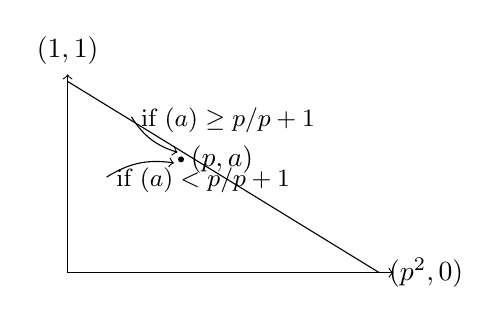
\begin{tikzpicture}[scale=0.9]
\draw[->] (0,0) -- (4.6,0) node[right]{};
\draw[->] (0,0) -- (0,2.8);
\node[above] at (0,2.8) {$(1,1)$};
\draw (0,2.7) -- (4.4,0);
\node[right] at (4.4,0) {$(p^2,0)$};
\fill (1.6,1.6) circle (1.2pt);
\node[right] at (1.6,1.6) {$(p,\ord a)$};
\draw[->] (0.9,2.2) to[bend right=20] (1.55,1.7);
\node[right] at (0.9,2.15) {\small if $\ord(a)\geq p/p+1$};
\draw[->] (0.55,1.35) to[bend left=20] (1.5,1.55);
\node[right] at (0.55,1.3) {\small if $\ord(a)<p/p+1$};
\end{tikzpicture}
\end{center}
and remarking that the construction of the canonical subgroup as subscheme of
the formal group consisted \uline{precisely of isolating} the factor of
$[p](X)$ corresponding to the first slope, when there is a first slope.

2. By Lubin (\cite{lubin67}), we know that if H is any finite subgroup of a one-parameter
formal group over $R_0$, then $X\to\prod_{x\in H} G(X,x)$ \uline{is} the
projection onto the quotient. Thus the non-zero points of order p on $E/H_0$
are of two sorts, the points $\prod_{x\in H_0} G(y,x)$ with $[p](y) = 0$,
$\ord(y) = \frac{\ord(a)}{p^2-p}$, and the points $\prod_{x\in H_0} G(z,x)$
where $[p](z)\in H_0$, $[p](z)\neq 0$. The first sort of point has ordinal
given by $\sum_{x\in H_0} \ord(G(y,x))$, and as $\ord(y)<\ord(x)$ for any
$x\in H_0$, this sum is just $p(\ord y) = \frac{\ord(a)}{p-1}$. The second
sort of point has ordinal $\sum_{x\in H_0} \ord(G(z,x))$. From the equation
$[p](z)\in H_0-\{0\}$, we see that
$\ord([p](z)) = \frac{1-\ord(a)}{p-1}$. The Newton polygon of
$[p](z) = x\in H_0-\{0\}$ is thus
\begin{center}
\begin{tikzpicture}[scale=0.9]
\draw[->] (0,0) -- (4.6,0);
\draw[->] (0,0) -- (0,2.8);
\node[left] at (0,2.7) {$(0,\frac{1-\ord(a)}{p-1})$};
\draw (0,2.7) -- (4.4,0);
\node[right] at (4.4,0) {$(p^2,0)$};
\fill (1.6,1.6) circle (1.2pt);
\node[right] at (1.6,1.6) {$(p,\ord(a))$};
\end{tikzpicture}
\end{center}
and hence z has either ordinal $\ord(a)/p^2-p$ or
$\frac{1-p\ \ord(a)}{p^2-p}$. In \uline{either} case, $\ord(z)<\ord(x)$ for any
$x\in H_0$. Hence the second sort of point has ordinal either
$\ord(a)/p-1$ or $(1-p\ \ord(a))/p-1$. Thus among the non-zero points of order
p on $E/H_0$, there are two distinct ordinals which occur, namely
$\ord(a)/p-1$ and $(1-p\ \ord(a))/p-1$, of which the \uline{greater} is
$(1-p\ \ord(a))/p-1$.

Thus by 1, $E/H_0$ has $\ord(a')<p/p+1$, and
$\frac{1-\ord(a')}{p-1} = \frac{1-p\ \ord(a)}{p-1}$, which proves 2. We note
that the image of $E$ is \uline{not} the canonical subgroup.

3. If we suppose $1/p+1<\ord(a)<p/p+1$, then on $E/H_0$ the first sort of
points of order p are the points $\prod_{x\in H_0} G(y,x)$ for each y such that
$[p](y) = 0$, $y\notin H_0$. As in 2, these points have ordinal
$\ord(a)/p-1$. The second sort are the points $\prod_{x\in H_0} G(z,x)$ where
$[p](z)\in H_0-\{0\}$, hence $[p](z)$ has ordinal $\frac{1-\ord(a)}{p-1}$. They
hypothesis $\ord(a)>1/p+1$ insures that the Newton polygon of
$[p](Z) = x\in H_0-\{0\}$ is
\begin{center}
\begin{tikzpicture}[scale=0.9]
\draw[->] (0,0) -- (4.6,0);
\draw[->] (0,0) -- (0,2.8);
\node[left] at (0,2.7) {$(0,\frac{1-\ord(a)}{p-1})$};
\draw (0,2.7) -- (4.4,0);
\node[right] at (4.4,0) {$(p^2,0)$};
\fill (1.6,1.6) circle (1.2pt);
\node[right] at (1.6,1.6) {$(p,\ord(a))$};
\end{tikzpicture}
\end{center}
hence $\ord(z) = \frac{1-\ord(a)}{p^2(p-1)}<\ord(x)$ for any $x\in H_0$, hence
the second sort of point has ordinal $1-\ord(a)/p(p-1)$. Thus $E/H_0$ has a
canonical subgroup, namely its points of order p of largest ordinal
$=\ord(a)/p-1$. Hence $\frac{1-\ord(a')}{p-1} = \ord(a)/p-1$, whence
$\ord(a') = 1-\ord(a)$, and the canonical subgroup \uline{is} the image of all
the points of order p on E.

4. If $\ord(a)\geq p/p+1$, the Newton polygon of $[p](X)$ is
\begin{center}
\begin{tikzpicture}[scale=0.9]
\draw[->] (0,0) -- (4.6,0);
\draw[->] (0,0) -- (0,2.8);
\node[above] at (0,2.7) {$(1,1)$};
\draw (0,2.7) -- (4.4,0);
\node[right] at (4.4,0) {$(p^2,0)$};
\fill (1.6,1.6) circle (1.2pt);
\node[right] at (1.6,1.6) {$(p,\ord(a))$};
\end{tikzpicture}
\end{center}
Hence all non-zero points of order p have the same ordinal $1/p^2-1$. The
points z such that $[p](z) = x$, $[p](x) = 0$, $x\neq 0$, have ordinal
$1/p^2(p^2-1)$, because the Newton polygon of $[p](z) = x$,
$\ord(x) = 1/p^2-1$, is
\begin{center}
\begin{tikzpicture}[scale=0.9]
\draw[->] (0,0) -- (4.6,0);
\draw[->] (0,0) -- (0,2.8);
\node[left] at (0,2.7) {$(0,1/p^2-1)$};
\draw (0,2.7) -- (4.4,0);
\node[right] at (4.4,0) {$(p^2,0)$};
\fill (1.6,1.6) circle (1.2pt);
\node[right] at (1.6,1.6) {$(p,\ord a)$};
\end{tikzpicture}
\end{center}
Thus for any subgroup $H_1$ of order p of E, the first sort of point of order
p has $\ord = \sum_{x\in H_1} \ord(G(y,x))\geq p\ \ord(y) = p/p^2-1$ (since
$\ord(y) = \ord(x)$ if $x\neq 0$). The second sort of point has ordinal
$p\cdot\ord(z) = 1/p(p^2-1)$, (because $\ord(z)<\ord(x)$ for any $x\in H_1$).
But $p/p^2-1>1/p(p^2-1)$, hence each $E/H_i$ \uline{has} a canonical subgroup,
which is the \uline{image} of $E$. Looking at the ordinals of the
\uline{non-canonical} points of order p on $E/H_1$, we have by \hyperref[ka:3.10.7]{(3.10.7.1)} the
equality $\ord(a')/p^2-p = 1/p(p^2-1)$, hence $\ord(a') = 1/p+1$.

5. We first remark that if $\ord(a)<p/p+1$, then $E' = E/H$ \uline{either}
has $\ord(a')>1/p+1$, or \uline{its} canonical subgroup is \uline{not} the
image of $E$ and hence $E'/H(E')\neq E$. Indeed, if $\ord(a)<1/p+1$, then as
noted in the proof of 2., the canonical subgroup is \uline{not} the image of
$E$. If $\ord(a) = 1/p+1$, then as proven in 4., $\ord(a')\geq p/p+1$. If
$\ord(a)>1/p+1$, then $\ord(a') = 1-\ord(a)$, and $1-\ord(a)>1/p+1$ because
$\ord(a)<p/p+1$. It remains to see that for each non-canonical subgroup $H_i$,
$i=1,\dots,p$, $E^{(i)} = E/H_i$ has $\ord(a^{(i)}) = \frac{1}{p}\ord(a_i)$,
and its canonical subgroup is the image of $E$.

Again we calculate the ordinals of the points of order p on $E/H_1$. The first
sort of points are all images of points of the canonical subgroup $H_0$ of E
(because $E = H_0\oplus H_1$ for $i=1,\dots,p$). For $y\in H_0-\{0\}$,
$\ord G(y,0) = \ord y = \frac{1-\ord(a)}{p-1}$, while
$\ord(G(y,x)) = \ord x = \frac{\ord(a)}{p^2-p}$ because $\ord(y)>\ord x$ if
$x\in H_1-\{0\}$. Hence the image of $y\in H_0-\{0\}$ has ordinal
$= \ord(y) + \sum_{x\in H_1-\{0\}} \ord(x) = \frac{1-\ord(a)}{p-1} +
p\cdot\frac{\ord(a)}{p^2-p} = \frac{1-\ord(a)}{p-1} + \frac{\ord(a)}{p}$.

What about the image of a point z such that $[p](z)\in H_1-\{0\}$? The Newton
polygon of $[p](Z) = x$, $x\in H_1-\{0\}$, is
\begin{center}
\begin{tikzpicture}[scale=0.9]
\draw[->] (0,0) -- (4.6,0);
\draw[->] (0,0) -- (0,2.8);
\node[left] at (0,2.7) {$(0,\frac{\ord(a)}{p^2-p})$};
\draw (0,2.7) -- (4.4,0);
\node[right] at (4.4,0) {$(p^2,0)$};
\fill (1.6,1.6) circle (1.2pt);
\node[right] at (1.6,1.6) {$(p,\ord a)$};
\end{tikzpicture}
\end{center}
hence $\ord(z) = \ord(a)/p^2(p^2-p) = \ord(x)/p^2$ for $x\in H_1-\{0\}$. Thus
$\ord(z)<\ord(x)$, hence the second sort of points of order p on $E^{(i)}$ have
ordinal $= p\cdot\ord(z) = \ord(a)/p(p^2-p)$. But
$\frac{1-\ord a}{p-1} + \frac{\ord(a)}{p} > \ord(a)/p(p^2-p)$ (because
$\ord(a)<p/p+1<p^2/p+1$), hence $E^{(i)}$ has a canonical subgroup, and
$\frac{1-\ord(a^{(i)})}{p-1} = \frac{1-\ord a}{p-1} + \frac{\ord(a)}{p}$, hence
$\ord(a^{(i)}) = \ord(a)/p$. This concludes the proof of 5., and also of
theorem \eqref{ka:3.10.7}.
\end{kaproof}

\sechead{3.11}{Applications to the congruences of Atkin - the U operator}

We maintain the notations of the previous section. As we have seen, for each
$r\in R_0$ having $\ord(r)<1/p+1$, the homomorphism
$\varphi\colon S(R_0,r^p,n,0)\to S(R_0,r,n,0)$ is \uline{finite}, and becomes
finite and flat of degree p when we tensor with K. Thus there is defined the
\uline{trace morphism}
\begin{kadispb}{3.11.1}
\tr_\varphi\colon S(R_0,r,n,0)\tens K\to S(R_0,r^p,n,0)\tens K.
\end{kadispb}
For $r=1$, $\varphi$ is itself finite flat of degree p, hence there is defined
\begin{kadispb}{3.11.2}
\tr_\varphi\colon S(R_0,1,n,0)\to S(R_0,1,n,0).
\end{kadispb}
In terms of q-expansion, we have
\begin{kadispb}{3.11.3}
(\tr_\varphi(f))(\mathrm{Tate}(q^n),\omega_{can},\alpha_n) = \sum_{\zeta_p=1} f(\mathrm{Tate}(\zeta q^{n/p}),\omega_{can},\tfrac{1}{p}\pi_\zeta(\alpha_n))
\end{kadispb}
where $\pi_\zeta(\alpha_n)$ denotes the induced level n structure on
$\mathrm{Tate}(\zeta q^{n/p})$, viewed as a quotient of $\mathrm{Tate}(q^n)$.
Equivalently, if we write
\begin{kadispb}{3.11.3.1}
f(\mathrm{Tate}(q^n),\omega_{can},\alpha_n) = \sum A_i(\alpha_n)q^i
\end{kadispb}
then we have the formula (in which $\alpha_n''$ is the level n structure on
$\mathrm{Tate}(q^n)$ obtained as the inverse image of $\pi_0(\alpha_n)$ on
$\mathrm{Tate}(q^{n/p})$ by the extension of scalars $q^{1/p}\to q$, compare
pp.32-33)
\begin{kadispb}{3.11.3.2}
(\tr_\varphi(f))(\mathrm{Tate}(q^n),\omega_{can},\alpha_n) = p\cdot\sum A_{pi}(\tfrac{1}{p}\alpha_n'')q^i.
\end{kadispb}
Notice that we have the relation, for any $f\in S(R_0,r,n,0)\tens K$,
\begin{kadispb}{3.11.3.3}
p\cdot T_p(f) = \tr_\varphi(I_p^*(f)) + \varphi(f)
\end{kadispb}
(where $I_p^*(f)(E/R,\omega,\alpha_n) \xlongequal{\mathrm{dfn}}
f(E/R,\omega,p\cdot\alpha_n)$), which should be viewed as the "canonical
p-adic lifting" of the Eichler-Shimura congruence relation (compare Deligne
\cite{deligne69}).

\begin{kathm}{Integrality Lemma}{3.11.4.}
For any $r\in R_0$ with $\ord(r)<1/p+1$, we have
$\tr_\varphi(S(R_0,r,n,0))\subset S(R_0,r^p,n,0)$ (although
$\varphi\colon S(R_0,r^p,n,0)\to S(R_0,r,n,0)$ is finite but \uline{not} flat if
$\ord(r)>0$!).
\end{kathm}

\begin{kaproof}
We may suppose $\ord(r)>0$, the case $r=1$ being trivial. It follows (from Tate
\cite{tate71}) that for \uline{any finite flat morphism} $\varphi\colon A\to B$ of rigid
algebras over K, we have $\tr_\varphi$ (power-bounded elements of $B$)
$\subset$ power-bounded elements of A. Thus we must show that the power-bounded
elements of $S(R_0,r,n,0)\tens K$ are \uline{precisely} $S(R_0,r,n,0)$. For
this, we introduce the finitely generated $R_0$-algebra $B =
H^0(\Mbar_n\tens R_0, \Sym(\w^{\otimes p-1}))/(E_{p-1}-r)$. Its p-adic
completion $\hat{B} \xlongequal{\mathrm{dfn}} \limleft B/p^N B$ \uline{is}
$S(R_0,r,n,0)$, and indeed via the isomorphism \eqref{ka:2.6.2.1}, B corresponds to the
$R_0$-submodule of $B^{\mathrm{rigid}}(R_0,r,n,0)$ consisting of all
\uline{finite} sums, which shows incidentally that B is a (free and hence) flat
$R_0$-module, and that $B/\mathfrak{m}B\cong \hat{B}/\mathfrak{m}\hat{B}$. The
fact that $E_{p-1}$ modulo $\mathfrak{m}$ has \uline{simple} zeros implies that
$B/\mathfrak{m}B$ is \uline{reduced}. (Indeed, $B/\mathfrak{m}B$ is
$H^0(M_n\tens R_0/\mathfrak{m}, \Sym(\w^{\otimes p-1}))/(E_{p-1})$, and if
$\sum_0^N f_i$ represents a nilpotent element, with minimal N, then a power of
$f_N$ is divisible by $E_{p-1}$, hence $f_N$ is divisible by $E_{p-1}$, which
contradicts the minimality of N.) We may thus conclude by the following lemma.
\end{kaproof}

\begin{kathm}{Lemma}{3.11.5.}
Let $R_0$ be a complete discrete valuation ring, B a flat finitely-generated
$R_0$-algebra such that $\hat{B}/\mathfrak{m}\hat{B}$ is reduced. Then the set
of power-bounded elements of $\hat{B}\tens K$ is $\hat{B}$.
\end{kathm}

\begin{kaproof}
Since $\hat{B}$ is flat over B, hence over $R_0$, we have
$\hat{B}\subset\hat{B}\tens K$, so the statement makes sense. By Tate, we know
that \uline{any} power-bounded element of $\hat{B}\tens K$ is \uline{integral}
over $\hat{B}$, so we must show that $\hat{B}$ is integrally closed in
$\hat{B}\tens K$. Let $\pi$ be a uniformizing parameter of $R_0$. If
$f\in\hat{B}$ and $f/\pi$ is \uline{integral} over $\hat{B}$, then clearing the
denominators in the equation shows that $f$ is a \uline{nilpotent} element of
$\hat{B}/\mathfrak{m}\hat{B}$, hence $f\in\mathfrak{m}\hat{B} = \pi\hat{B}$.
\end{kaproof}

\kaitemb{3.11.6.} We now define Atkin's operator
$U\colon S(R_0,r^p,n,0)\tens K\to S(R_0,r^p,n,0)$ to be the composite
\[
S(R_0,r^p,n,0)\tens K \hookrightarrow S(R_0,r,n,0)\tens K
\xrightarrow{\frac{1}{p}\tr_\varphi} S(R_0,r^p,n,0)\tens K.
\]
Thus if $f\in S(R_0,r^p,n,0)$ has q-expansions
\begin{kadispb}{3.11.6.1}
f(\mathrm{Tate}(q^n),\omega_{can},\alpha_n) = \sum_i A_i(\alpha_n)q^i
\end{kadispb}
then $U f\in S(R_0,r^p,n,0)\tens K$ has q-expansions
\begin{kadispb}{3.11.6.2.}
(U f)(\mathrm{Tate}(q^n),\omega_{can},\alpha_n) = \sum A_{pi}(\tfrac{1}{p}\alpha_n'')\cdot q^i.
\end{kadispb}
[This formula shows that $U(S(R_0,1,n,0))\subset S(R_0,1,n,0)$]. It is
\uline{not} true in general that $U(S(R_0,1,n,0))\subset S(R_0,r^p,n,0)$, but
the situation is as good as if it were true, as Dwork was the first to realize.

\begin{kathm}{Lemma}{3.11.7.}
(Dwork) Suppose $p\geq 7$, and suppose $r\in R_0$ satisfies the inequality
\[
\frac{2}{3(p-1)} < \ord(r) < \frac{1}{p+1}.
\]
Then the $R_0$-submodule $S(R_0,r^p,n,0) + U(S(R_0,r^p,n,0))$ of
$S(R_0,r^p,n,0)\tens K$ is $U$-stable.
\end{kathm}

\begin{kathmstar}[3.11.8]{Remark 3.11.8.}
The point is that the submodule $S(R_0,r^p,n,0) + U(S(R_0,r^p,n,0))$ contains
$S(R_0,r^p,n,0)$ and is contained in $\frac{1}{p}S(R_0,r^p,n,0)$, hence it
defines the \uline{same} topology on $S(R_0,r^p,n,0)\tens K$ as
$S(R_0,r^p,n,0)$. Thus in an \uline{equivalent} norm on
$S(R_0,r^p,n,0)\tens K$, U has operator norm $\leq 1$.
\end{kathmstar}

\begin{kaproof}
Let's use the representation \eqref{ka:2.6.2.1} of elements of $S(R_0,r^p,n,0)$ in the
form $f = \sum_{a\geq 0}\frac{r^{pa}\cdot b_a}{(E_{p-1})^a}$. The hypothesis
insures that for $a\geq 2$, $\ord(r^{pa}/p\cdot r^a)>0$, and hence
\begin{kadispb}{3.11.9.}
f = b_0 + \frac{r^p\cdot b_1}{E_{p-1}} + p\cdot(\text{an element of }
\frac{r^{2(p-1)}}{p}S(R_0,r,n,0)).
\end{kadispb}
Because $pU = \tr_\varphi$ maps $S(R_0,r,n,0)$ to $S(R_0,r^p,n,0)$, we have
\begin{kadispb}{3.11.10.}
U(f) = U(b_0) + U\left(\frac{r^p b_1}{E_{p-1}}\right) + \text{an element of }
\frac{r^{2(p-1)}}{p}S(R_0,r^p,n,0).
\end{kadispb}
Since $b_0$ is just a \uline{constant}, we have $U(b_0) = b_0$, and hence it
suffices to show that for any $b_1\in H^0(\Mbar_n\tens R_0,\w^{\otimes p-1})$,
we have
\begin{kadispb}{3.11.11}
U^2\left(\frac{r^p b_1}{E_{p-1}}\right)\subset S(R_0,r^p,n,0) + U(S(R_0,r^p,n,0)).
\end{kadispb}
For this, notice that $rb_1/E_{p-1}$ lies in $S(R_0,r,n,0)$, hence
\begin{kadispb}{3.11.12.}
\tr_\varphi\left(\frac{rb_1}{E_{p-1}}\right) = \sum_{a\geq 1}\frac{r^{pa}b_a'}{(E_{p-1})^a}.
\end{kadispb}
The hypotheses insure that $\ord(\frac{r^{p-1}}{p}\cdot r^{pa}/p\cdot r^a)>0$
if $a\geq 2$, and hence
\begin{kadispb}{3.11.13}
U\left(\frac{r^p b_1}{E_{p-1}}\right) &= \frac{r^{p-1}}{p}\tr_\varphi\left(\frac{rb_1}{E_{p-1}}\right) = \frac{r^{p-1}}{p}\left(b_0' + \frac{r^p b_1'}{E_{p-1}}\right) + \\
&\quad + p\left(\text{an element of } \frac{r^3(p-1)}{p^2}S(R_0,r,n,0)\right).
\end{kadispb}
Notice that $U\left(\frac{r^p b_1}{E_{p-1}}\right)$ has q-expansions divisible by
$r^p$, as does $p(\text{any element of } S(R_0,r^p,n,0))$, and hence so does
\[
\begin{split}
(r^{p-1}/p)&\left(b_0' + \frac{r^p b_1'}{E_{p-1}}\right) \\
&= \frac{r^{p-1}}{p}\left(\frac{b_0' E_{p-1} + r^p b_1'}{E_{p-1}}\right),
\end{split}
\]
and hence so does $\frac{r^{p-1}}{p}(b_0' E_{p-1} + r^p b_1')$. By the
q-expansion principle\index{q-expansion principle}, there exists an element
$b_1''\in H^0(\Mbar_n\tens R_0,\w^{\otimes p-1})$ such that
$\frac{r^{p-1}}{p}(b_0' E_{p-1} + r^p b_1') = r^p b_1''$, hence
$\frac{r^{p-1}}{p}\left(b_0' + \frac{r^p b_1'}{E_{p-1}}\right) =
\frac{r^p b_1''}{E_{p-1}}$, hence
\[
U\left(\frac{r^p b_1}{E_{p-1}}\right) = \frac{r^p b_1''}{E_{p-1}} +
p\cdot(\text{an element of } \frac{r^3(p-1)}{p^2}S(R_0,r,n,0)).
\]
Again using the fact that $pU = \tr_\varphi$ maps $S(R_0,r,n,0)$ to
$S(R_0,r^p,n,0)$, we find
\[
U^2\left(\frac{r^p b_1}{E_{p-1}}\right) = U\left(\frac{r^p b_1''}{E_{p-1}}\right)
+ \text{an element of } S(R_0,r^p,n,0),
\]
which proves \eqref{ka:3.11.11} and the lemma.
\end{kaproof}

\sechead{3.12}{p-adic Hecke operators}

For any prime number $\ell$ which is prime to both p and to the level n, we
may define $T_\ell$ on $S(R_0,r,n,k)$ by the usual formula
\begin{kadispb}{3.12.1}
(T_\ell f)(E/R,\omega,\alpha_n,Y) = \ell^{k-1}\sum f(E_K/R,\pi^*(\omega),\pi(\alpha_n),\pi^*(Y))
\end{kadispb}
the sum extended to the $\ell+1$ subgroups K of order $\ell$. The various
$T_\ell$ commute with each other, and for $k=0$ they all commute with U.

We may consider the "spectral decomposition" of the K-Banach\index{Banach space} space
$S(R_0,r^p,n,0)\tens K$ with respect to U (which is completely continuous,
because the inclusion $S(R_0,r^p,n,0)\tens K$ into $S(R_0,r,n,0)\tens K$ is).
For any rational number v, the subspace
\begin{kadispb}{3.12.3}
\bigcup_{m\geq 1}\ \bigcup_{\substack{\alpha\in K^{\mathrm{alg.}}\\ \text{of ordinal } v}} \Ker(U-\alpha)^m
\end{kadispb}
of $S(R_0,r^p,n,0)\tens K$ is \uline{finite-dimensional}, and is stable by U
and the $T_\ell$. By Dwork's lemma \eqref{ka:3.11.7}, this subspace is reduced to
$\{0\}$ unless $v\geq 0$. The first interesting case is thus to take $v=0$, the
so-called "unit-root subspace" of $S(R_0,r^p,n,0)\tens K$. [Notice that this
unit root subspace is \uline{independent} of the choice of $r\in R_0$ with
$1/p+1>\ord(r)>0$, because U maps $S(R_0,r,n,0)\tens K$ to
$S(R_0,r^p,n,0)\tens K$, i.e. it \uline{improves} growth conditions. Thus if
$f\in S(R_0,r,n,0)\tens K$ is annihilated by $(U-\alpha)^m$, and $\alpha\neq 0$,
then f is a $K(\alpha)$-linear combination of $U(f), U^2(f),\dots, U^m(f)$,
hence in fact $f\in S(R_0,r^p,n,0)\tens K,\dots$.]

\begin{kathm}{Lemma}{3.12.4.}
(Dwork) Hypotheses as in \eqref{ka:3.11.7}, the dimension of the unit root subspace of
$S(R_0,r^p,n,0)\tens K$ is \uline{at most}
$\dim_K H^0(\Mbar_n\tens K,\w^{\otimes p-1})$.
\end{kathm}

\begin{kaproof}
The dimension of the unit root subspace is the number of unit zeros of the
Fredholm determinant\index{Fredholm determinant} of U, which by \eqref{ka:3.11.8} lies in $R_0[[T]]$, hence this
dimension is also the degree of this Fredholm determinant reduced modulo
$\mathfrak{m}$, which is to say the degree of the determinant of U on
$(S(R_0,r^p,n,0) + U(S(R_0,r^p,n,0))\tens_{R_0} R_0/\mathfrak{m}$.

But for $f\in S(R_0,r^p,n,0)$, $f = \sum_{a\geq 0}\frac{r^{pa}b_a}{(E_{p-1})^a}$,
we have $U(f)\equiv b_0 + U\left(\frac{r^p b_1}{E_{p-1}}\right)$ modulo
$\mathfrak{m}\cdot S(R_0,r^p,n,0)$ and
$U^2(f)\equiv U\left(\frac{r^p b_1''}{E_{p-1}}\right)$ modulo
$\mathfrak{m}\cdot S(R_0,r^p,n,0)$. Thus the \uline{image} of U on
$(S(R_0,r^p,n,0) + U(S(R_0,r^p,n,0))\tens R/\mathfrak{m}$ is \uline{spanned} by
the images under U of all elements $b_0\in H^0(\Mbar_n\tens R_0,\cO)$ and
$\frac{r^p b_1}{E_{p-1}}$ with
$b_1\in B(R_0,n,k,1)\xrightarrow{\sim}
H^0(\Mbar_n\tens R_0,\w^{\otimes p-1})/E_{p-1}H^0(\Mbar_n\tens R_0,\cO)$. Thus
the rank of U on
$(S(R_0,r^p,n,0) + U(S(R_0,r^p,n,0))\tens R_0/\mathfrak{m}$ is at most the
K-dimension of $H^0(\Mbar_n\tens K,\w^{\otimes p-1})$.
\end{kaproof}

\sechead{3.13}{Interpretation of Atkin's congruences on $j$}

We denote by $j$ the absolute j-invariant, viewed as a modular function of
level one, defined over $\Z$, having a first order pole at infinity. As is well
known, $p\cdot T_p(j)$ lies in $\Z[j]$. By inverse image we may view both $j$
and $p\cdot T_p(j)$ as elements of $M(R_0,r,n,0)$ for \uline{any} $r\in R$. We
may also view $\varphi(j)$ as an element of $M(R_0,r,n,0)$, for any $r\in R_0$
having $\ord(r)<p/p+1$ [indeed, $\varphi(j)(E,Y) = j(E/H)$, H the canonical
subgroup]. Subtracting, we define
$p\cdot U(j) = p\cdot T_p(j) - \varphi(j)\in M(R_0,r,n,0)$. Because j has only a
first order pole at $\infty$, $U(j)$ is holomorphic at infinity, indeed its
q-expansion is
\begin{kadispb}{3.13.1}
U(j)(\mathrm{Tate}(q)) = \sum_{n\geq 0} c(pn)q^n, \quad\text{where}
\end{kadispb}
\begin{kadispb}{3.13.2}
j(\mathrm{Tate}(q)) = \sum_{n\geq -1} c(n)q^n = \frac{1}{q} + 744 + \cdots.
\end{kadispb}
Thus $U(j)$ lies in $S(\Z_p,1,n,0)$, and $p\cdot U(j)$ lies in
$S(R_0,r,n,0)$ for any $r\in R_0$ having $\ord(r)<p/p+1$. Combining this
observation with the remark \eqref{ka:3.11.8}, we see that for \uline{every} $m\geq 1$,
we have
\[
U^m(j)\in S(\Z_p,1,n,0)\cap p^{-2}S(R_0,r,n,0).
\]

Let us examine explicitly the congruence consequences of the innocuous
statement "$U(j)\in S(\Z_p,1,n,0)\cap p^{-1}S(R_0,r,n,0)$ whenever
$\ord(r)<p/p+1$". Suppose that $p\neq 2,3$, so that we may work directly with
$S(R_0,r,1,0)$ via its basis as constructed in \eqref{ka:2.6.2.1}. We may write
\begin{kadispb}{3.13.3.0}
U(j) = \sum_{a\geq 0}\frac{b_a}{(E_{p-1})^a}, \quad b_a\in B(\Z_p,1,0,a).
\end{kadispb}
For $r\in R_0$ with $\ord(r)<p/p+1$, we have $p\cdot b_a\in r^a B(R_0,1,0,a)$,
hence we have $pb_a\in p^{\{ap/p+1\}}B(\Z_p,1,0,a)$, where $\{ap/p+1\}$ denotes
the least integer $\geq ap/p+1$. Thus $b_0\in\Z_p$, $b_1\in B(\Z_p,1,0,1)$,
$b_a\in p^{a-1}B(\Z_p,1,0,a)$ for $2\leq a\leq p$, $b_{p+1}\in
p^{p-1}B(\Z_p,1,0,a),\dots$, certainly $b_a\in p^{n+1}B(\Z_p,0,a)$ if $a>p^n$,
for $n\geq 1$. Thus
\begin{kadispb}{3.13.3.1}
U(j) \equiv \sum_{a=0}^{p^n}\frac{b_a}{(E_{p-1})^a} \quad \text{modulo } p^{n+1}S(\Z_p,1,1,0)
\end{kadispb}
\begin{kadispb}{3.13.3.2}
U(j) \equiv \frac{\sum_{a=0}^{p^n} b_a\cdot(E_{p-1})^{p^n-a}}{(E_{p-1})^{p^n}} \quad \text{modulo } p^{n+1}S(\Z_p,1,1,0).
\end{kadispb}
Using the fact that $E_{p-1}$ has q-expansion $\equiv 1\ (p)$, and hence that
$(E_{p-1})^{p^n}$ has q-expansion $\equiv 1\ (p^{n+1})$, we deduce that for
$p\neq 2,3$, the q-expansion of $U(j)$ is congruent mod $p^{n+1}$ to the
q-expansion of a true modular form\index{modular form} of level one, defined over $\Z$, holomorphic
at $\infty$, of weight $p^n(p-1)$. In fact, using $(E_{p-1})^{p^n}$ to kill the
constant term, we find that $U(j) - 744$ has q-expansion congruent mod
$p^{n+1}$ to the q-expansion of a cusp form of level one and weight $p^n(p-1)$,
defined over $\Z$, a result obtained independently by Koike \cite{koike}.

We now return to the properly Atkinesque aspects of the $U^n(j)$, and their
interpretation.

\begin{kathm}{Lemma}{3.13.4.}
Suppose there exists a p-adic unit $a\in\Z_p$ such that for every $m\geq 1$, we
have the q-expansion congruences
\[
U^{m+1}(j-744) \equiv a\ U^m(j-744) \quad \text{modulo } p^m \text{ in q-expansion}
\]
i.e., $c(p^{m+1}i)\equiv ac(p^m i) \quad \text{modulo } p^m \text{ for all }
m\geq 1$.

Let $c_\infty(i) = \lim_m a^{-m}c(p^m i)$. Then for $r\in R_0$ having
$\ord(r)<p/p+1$, there is a unique element
"$\lim$" $a^{-m}U^m(j-744)\in S(\Z_p,1,n,0)\cap p^{-2}S(R_0,r,n,0)$ which is of
level one (i.e., invariant under $\GL_2(\Z/n\Z)$), whose q-expansion is
$\sum_{m\geq 1} c_\infty(i)q^i$, and which is \uline{fixed} by $a^{-1}U$.
\end{kathm}

\begin{kaproof}
By \eqref{ka:2.7}, the hypothesis is in fact equivalent to the congruences
\begin{kadispb}{3.13.4.1}
(a^{-1}U)^{m+1}(j-744) \equiv (a^{-1}U)^m(j-744) \quad \text{modulo } p^m S(\Z_p,1,n,0).
\end{kadispb}
Let's write the expression of $(a^{-1}U)^m(j-744)$ in terms of the \uline{base}
of $S(\Z_p,1,n,0)$:
\begin{kadispb}{3.13.4.2}
(a^{-1}U)^m(j-744) = \sum_{a\geq 0}\frac{b_a(m)}{(E_{p-1})^a}, \quad b_a(m)\in B(\Z_p,n,0,a).
\end{kadispb}
Then we have the congruences $b_a(n+1)\equiv b_a(n)$ modulo
$p^n B(\Z_p,n,0,a)$, we may define $b_a(\infty) = \lim_m b_a(m)\in
B(\Z_p,n,0,a)$. But for any $r\in R_0$ with $\ord(r)<1/p+1$, we have
$p^2 b_a(m)\in r^a B(R_0,n,0,a)$, hence $p^2 b_a(\infty)\in r^a B(R_0,n,0,a)$.
Varying $(R_0,r)$, we see that in fact $p^2 b_a(\infty)$ lies in
$p^{\{ap/p+1\}}B(\Z_p,n,0,a)$, where $\{x\}$ denotes the least integer $\geq x$,
(i.e., $\{x\} = -[-x]$). Hence $\sum\frac{b_a(\infty)}{(E_{p-1})^a}
\xlongequal{\mathrm{dfn}} \text{"lim"}(a^{-1}U)^m(j-744)$ lies in
$S(\Z_p,1,n,0)\cap p^{-2}S(R_0,r,n,0)$, and in $S(\Z_p,1,n,0)$ it is the
\uline{limit} (in the Banach\index{Banach space} space topology of $(a^{-1}U)^m(j-744)$.

The last two assertions are obviously true for $r=1$, by passage to the limit,
and follow for any $r$ of $\ord(r)<p/p+1$ because the canonical map
$S(R_0,r,n,0)\to S(R_0,1,n,0)$ is injective.
\end{kaproof}

\begin{kathmstar}{Remark 3.13.5.}
The hypotheses of the lemma are in fact \uline{satisfied} for $p=13$, a
striking result due to Atkin.
\end{kathmstar}

\kaitem{3.13.6} Using the fact that the twelfth power $\w^{\otimes 12}$ of $\w$
descends to the invertible sheaf $\cO(1)$ on the projective j-line over $\Z$,
one can copy the construction of a basis of $S(R_0,r,n,0)$, $n\geq 3$, to get a
\uline{basis} of $S(R_0,r,1,0) \xlongequal{\mathrm{dfn}}
S(R_0,r,n,0)^{\GL_2(\Z/n\Z)}$ for primes $p\equiv 1 \bmod 12$. Then one can
copy the proof given in (\cite{dwork-involume}) to show that the dimension of the unit root
subspace of $S(R_0,r,1,0)\tens K$ is \uline{at most}
$\dim H^0(\PP^1,\w^{\otimes p-1}) = \dim H^0(\PP^1,\cO(\frac{p-1}{12})) =
1 + \frac{p-1}{12}$, for $p\equiv 1 \bmod 12$. In particular, for $p=13$, the
unit root space has a base consisting of the constant function and the function
"$\lim$"$(a^{-1}U)^n(j-744)$, and this latter function is necessarily the
\uline{unique} "unit root cusp form" in $S(R_0,r,1,0)$. This unicity, together
with the stability of the space of unit root cusp forms under the Hecke
operators $T_\ell$, $\ell\neq 13$, gives a startling result of Atkin.

\begin{kathm}{Theorem}{3.13.7.}
(Atkin) The 13-adic modular function "$\lim$"$(a^{-1}U)^n(j-744) =
\sum_{1\leq i} c_\infty(i)q^i$ is a simultaneous eigenfunction of all the Hecke
operators $T_\ell$, $\ell\neq 13$.
\end{kathm}

\kaitem{3.13.8} Using the fact that $\w^{\otimes 2}$ descends to the invertible
sheaf $\cO(1)$ on the projective $\lambda$-line $\Mbar_2$ over $\Z[1/2]$, one
may construct as above a base of $S(R_0,r,2,0)$, and prove as above that the
unit root subspace of $S(R_0,r,2,0)\tens K$ has dimension at most
$\dim H^0(\Mbar_2,\w^{\otimes p-1}) = \dim H^0(\PP^1,\cO(\frac{p-1}{2})) =
1 + \frac{p-1}{2}$, for p odd. In fact, Dwork has proven that in this case the
dimension is exactly $1 + \frac{p-1}{2}$, (cf. his expos\'e in this volume).

\kaitem{3.13.9} Dwork's result implies that for $p\equiv 1 \bmod 12$, the
dimension of the unit root subspace of $S(R_0,r,1,0)$ is \uline{precisely}
$1 + \frac{p-1}{12}$, and hence that there are precisely $\frac{p-1}{12}$
independent unit root cusp forms in $S(R_0,r,1,0)$.

For $p=13$, this fact together with the "accident" $c(13)\neq 0 \bmod 13$,
\uline{implies} Atkin's result that a and "$\lim_m$"$(a^{-1}U)^m(j-744)$ exist.


\chapterhead{4}{p-adic representations and congruences for modular forms}

\sechead{4.1}{p-adic representations and locally free sheaves}

Let $q$ be a power of $p$, $k$ a perfect field containing $\F_q$, $\W_n(k)$
its ring of Witt vectors\index{Witt vector} of length $n$, and $S_n$ a flat affine $\W_n(k)$-scheme
whose special fibre is normal, reduced and irreducible. Suppose that $S_n$
admits an endomorphism $\varphi$ which induces the q-th power mapping on the
special fibre. [If $S_n$ is affine and smooth over $\W_n(k)$, then such a
$\varphi$ always exists.]

\begin{kathm}{Proposition}{4.1.1}
There is an equivalence of categories between the category of finite free
$\W_n(\F_q)$-modules $M$ on which $\pi_1(S_n)$ acts continuously, and the
category of pairs $(H,F)$ consisting of a locally free sheaf of finite rank
$H$ on $S_n$ together with an isomorphism $F\colon\varphi^*(H)\to H$.
\end{kathm}

\begin{kaproof}[Construction-proof]
Given a representation $M$ of $\pi_1(S_n)$, let $T_n$ be a finite \'etale galois
$S_n$-scheme such that the representation factors through $\Aut(T_n/S_n)$.
Because $T_n$ is \'etale over $S_n$, there is a unique $\varphi$-linear
endomorphism of $T_n$ which induces the q-th power endomorphism of
$T_n\times_{\W_n(k)}k$, which we denote by $\varphi_T$. By unicity, $\varphi_T$
commutes with $\Aut(T_n/S_n)$. Let $H_T$ be the $T_n$-module
$M\tens_{\W_n(\F_q)}\cO_{T_n}$, and let $F_T$ be the $\varphi_T$-linear
endomorphism of $H_T$ defined by $F_T(m\tens f)=m\tens\varphi_T(f)$. For each
$g\in\Aut(T_n/S_n)$, we define $g(m\tens f)=g(m)\tens(g^{-1})^*(f)$, thus
defining an action of $\Aut(T_n/S_n)$ on $(H_T,F_T)$. By descent, it follows
that there is a unique $(H,F)$ on $S_n$ whose inverse image on $T_n$ is
$\Aut(T_n/S_n)$-isomorphic to $(H_T,F_T)$. The construction
$M\rightsquigarrow(H,F)$ defines the functor we will prove to be an equivalence.
Notice that we can recover $M$ as the fixed points of $F_T$ acting as
$\varphi$-linear endomorphisms of the module of global sections of $H_T$, hence
our functor is fully faithful. To show that it is an equivalence, we must show
that any $(H,F)$ arises in this way, or, in concrete terms, we must show that
given $(H,F)$, there exists a finite \'etale covering $T_n$ of $S_n$ over which
$H$ admits a basis of F-fixed points. We proceed by induction on the integer
$n$.

Suppose first $n=1$. Then $S$ is a k-scheme, and $(H,F)$ is a locally free
finite rank S-module $H$ together with a q-linear endomorphism $F$ of $H$ which
gives an isomorphism $F\colon H^{(q)}\to H$. For any S-scheme $T$, the inverse
image module $H_T$ carries the inverse image q-linear map $F_T$, defined by
$(F_T(h\tens t)=F(h)\tens t^q$, which gives an isomorphism
$F_T\colon H_T^{(q)}\to H_T$.

Notice that the functors on S-schemes
\[
\begin{cases}
X(T) = \text{global sections of } H_T \\
Y(T) = \text{bases of } H_T\ (\cO_T\text{-isomorphisms }(\cO_T)^r\to H_T,\text{ where } r=\rank(H)) \\
Z(T) = \text{bases of } H_T \text{ consisting of fixed points of } F_T
\end{cases}
\]
are all \uline{representable}, the first by $\Spec_S(\Sym(H))$, the second by
the open subset of the $r=\rank(H)$-fold product
$X^{(r/S)}=X\times_S X\times\cdots\times_S X$ over which the tautological map
$(\cO_{X^{(r/S)}})^r\to H_{X^{(r/S)}}$ is an isomorphism, the third by the
closed subscheme of $Y$ over which the universal basis is fixed by $F_Y$. We
must show that $Z$ is finite and \'etale over $S$. \uline{This} problem is local
on $S$, hence we may assume $S$ affine and $H$ free. Choose a basis
$h_1,\dots,h_r$ of $H$, and let $(a_{ij})$ be the invertible matrix of
$F\colon F(h_i)=\sum_j a_{ji}h_j$.

Consider the functor on S-schemes
\[
Y'(T) = \text{sections of } H_T \text{ fixed by } F_T.
\]
It is representable by a scheme finite and \'etale of rank $q^r$ over $S$,
because a section $\sum_i X_ih_i$ of $H$ is F-fixed if and only if
$\sum_j X_jh_j=\sum_i (X_i)^q\sum_j a_{ji}h_j$, thus $Y'$ is the closed
subscheme of $\mathbb{A}^r_S$ defined by the equation
\[
X_j = \sum_i a_{ji}(X_i)^q,\qquad j=1,\dots,r .
\]
Because the matrix $(a_{ij})$ is invertible, if we denote by $(b_{ij})$ its
\uline{inverse}, the equations are the same as the equations
\[
(X_i)^q = \sum_j b_{ij}X_j\qquad i=1,\dots,r ,
\]
which define a finite \'etale S-scheme of rank $q^r$.

The scheme $Z$ is the \uline{open} subscheme of $Y'^{(r/S)}=Y'\times_S\cdots
\times_S Y'$ where the universal r-tuple of F-fixed sections form a base of
$H$, and hence $Z$ is \uline{\'etale} over $S$. It remains to check that $Z$ is
proper over $S$, and non-void. By the valuative criterion, we must show that for
any valuation ring $V$ over $S$, any F-fixed basis of $H_K$ ($K$ the fraction
field of $V$) prolongs to an F-fixed basis of $H_V$. Because the scheme $Y'$ of
fixed points is \uline{finite} over $S$, each basis element prolongs to a
unique F-fixed section of $H_V$. To see that the corresponding map
$V^r\to H_V$ is an isomorphism, we look at its \uline{determinant}, which
reduces us to the case of a rank one module. Then the matrix of $F$ is
$F(h_1)=ah_1$, with $a$ invertible in $V$, and an F-fixed basis of $H_K$ is a
vector $k\cdot h_1$, with $k\in K$ satisfying $k=ak^p$. As $a\in V$ is
invertible in $V$, any such $k$ is an invertible element of $V$, hence
$k\cdot h_1$ "is" an F-fixed base of $H_V$.

It remains to see that $Z$ is non-empty. As its formation commutes with
arbitrary change of base $S'\to S$, it's enough to check the case when $S$ is
the spectrum of an algebraically closed field. But a finite-dimensional vector
space over an algebraically closed field with a q-linear \uline{automorphism}
is always spanned by its fixed points (Lang's trick; cf.\cite{katz69}) and the set of
fixed bases is a $\GL_r(\F_q)$-torseur. Thus $Z$ is finite \'etale of rank
$=\#\GL_r(\F_q)$ over $S$, and the action of $\GL_r(\F_q)$ on $Z$ (induced by
its action on the functor of F-fixed bases) makes $Z$ into a
$\GL_r(\F_q)_S$-torseur. The cohomology class of this torseur is an element of
$H^1_{\text{\'et}}(S,\GL_r(\F_q))=\Hom(\pi_1(S),\GL_r(\F_q))$ which is none
other than the desired representation. This concludes the construction-proof
for $n=1$.

Suppose the result known for $n-1$. Then there is a finite \'etale covering
$T_{n-1}$ of $S_{n-1}=S_n\times_{\W_n(k)}\W_{n-1}(k)$ over which $H/p^{n-1}H$
admits a basis of F-fixed points. There is a unique finite \'etale covering
$T_n$ of $S_n$ such that $T_n\times_{S_n}S_{n-1}$ is $T_{n-1}$, and replacing
$S_n$ by $T_n$ we may suppose that $H/p^{n-1}H$ admits a basis of F-fixed
points. Let $h_1,\dots,h_r$ be a basis of $H$ which \uline{lifts} an F-fixed
basis of $H/p^{n-1}H$ ($S_n$ is affine!). Writing
$\underline{h}=\begin{pmatrix}h_1\\ \vdots\\ h_r\end{pmatrix}$, we have
$F(\underline{h})=(1+p^{n-1}\Delta)\underline{h}$. In order for
$(1+p^{n-1}E)\cdot\underline{h}$ to be an F-fixed basis, we must have
\[
(1+p^{n-1}\cdot\varphi(E))\cdot(1+p^{n-1}\Delta)\underline{h} = (1+p^{n-1}E)\underline{h}
\]
or equivalently ($S_n$ being flat over $\W_n(k)$)
\[
\varphi(E)+\Delta\equiv E \bmod (p),
\]
which is a set of $r^2$ Artin-Schreier equations $(e_{ij})^q-e_{ij}=-\Delta_{ij}$
over $S_1=S_n\times_{\W_n(k)}k$. On a finite \'etale covering $T_1$ of $S_1$,
these equations admit solutions, and hence on the unique finite \'etale covering
$T_n$ of $S_n$ such that $T_n\times_{S_n}S_1=T_1$, the module $H_{T_n}$ admits
an F-fixed basis.
\end{kaproof}

\begin{kathmstar}[4.1.2.1]{Remarks 4.1.2.1}
The operation "tensor product" in the category of representations of
$\pi_1(S_n)$ in finite free $\W_n(\F_q)$ modules corresponds to the tensor
product $(H,F)\tens(H',F')=(H\tens_{S_n}H',F\tens F')$, defined by
$(F\tens F')(h\tens h')=F(h)\tens F'(h')$.
\end{kathmstar}

\kaitem{4.1.2.2} The "internal Hom" in the category of representations
corresponds to the internal Hom defined by
$\underline{\Hom}((H,F),(H_1,F_1))=(\underline{\Hom}(H,H_1),F_2)$ where $F_2$ is
the unique $\varphi$-linear endomorphism of $\underline{\Hom}(H,H_1)$ such that
for $h\in H$, $f\in\underline{\Hom}(H,H_1)$, we have $F_2(f)(F(h))=F_1(f(h))$.
In particular, $\underline{\Hom}((H,F),(\cO,\varphi))$ is the "contragredient"
$(\widetilde{H},\widetilde{F})$, defined by the requirement that for $h\in H$,
$\widetilde{h}\in\widetilde{H}$, we have
$\langle F(h),\widetilde{F}(\widetilde{h})\rangle=\varphi(\langle h,\widetilde{h}\rangle)$.

\kaitem{4.1.2.3} Because $S_1$ is normal, reduced and irreducible, a
representation of $\pi_1(S_m)=\pi_1(S_1)$ is just a suitably unramified
representation of the Galois group of the function field of $S_1$. Thus for any
non-void open set $U\subset S_n$, the functor "restriction" from the category of
representations of $\pi_1(S_n)$ to the category of representations of
$\pi_1(U)$ is \uline{fully faithful}. Hence the functor "restriction" from the
category of $(H,F)$'s over $S_n$ to the category of those over $U$ is \uline{fully
faithful}.

\sechead{4.2}{Application to modular schemes}

\kaitemb{4.2.0.} Let $n\geq 3$, $p$ a prime not dividing $n$, $q$ a power of $p$
such that $q\equiv 1 \bmod n$, and choose an \uline{isomorphism} between $\mu_n$
and $\Z/n\Z$ over $\W(\F_q)$, i.e. choose a primitive n'th root of unity
$\zeta$. Let $S_m^\zeta$ (resp. $\overline{S}_m^\zeta$) be the open subset of
$M_n\tens\W_m(\F_q)$ (resp. of $\Mbar_n\tens\W_m(\F_q)$) where $E_{p-1}$ is
invertible \uline{and} where the e.m. pairing on the basis of ${}_nE$ has the
value $\zeta$, i.e. where the \uline{determinant} of the level n structure is
the chosen isomorphism of $\Z/n\Z$ with $\mu_n$. The schemes $S_m^\zeta$ (resp.
$\overline{S}_m^\zeta$) are smooth affine $\W_m(\F_q)$ schemes with
geometrically connected fibres. In the notation of \eqref{ka:2.9}, we have
$M_n(\W_m(\F_q),1)=\bigcup S_m^\zeta$, the union taken over the \uline{primitive}
n'th roots of unity, and $\Mbar_n(\W_m(\F_q),1)=\bigcup\overline{S}_m^\zeta$.

Let $\sigma$ denote the Frobenius\index{Frobenius} automorphism of $\W_m(\F_q)$. We have
$\sigma(\zeta)=\zeta^p$, and hence $S_m^{\zeta^p}=(S_m^\zeta)^{(\sigma)}$,
$\overline{S}_m^{\zeta^p}=(\overline{S}_m^\zeta)^{(\sigma)}$. The endomorphism
$\varphi$ of $\Mbar_n(\W_m(\F_q),1)$ defined by "division by the canonical
subgroup" does not respect the various $\overline{S}_m^\zeta$, but rather it
maps $\overline{S}_m^\zeta$ to $\overline{S}_m^{\zeta^p}$ (because modulo $p$,
the canonical subgroup\index{canonical subgroup} is the kernel of absolute Frobenius). As
$\overline{S}_m^{\zeta^p}=(\overline{S}_m^\zeta)^{(\sigma)}$, we may and will
view $\varphi$ as a $\sigma$-linear endomorphism of each $S_m^\zeta$, which
modulo $p$ becomes the p'th power mapping. In a similar fashion, the
endomorphism $\varphi$ of the invertible sheaf $\w^{\otimes k}$ on
$\Mbar_n(\W_m(\F_q),1)$, defined by
$\varphi(f)(E,\omega,\alpha_n)=f(E/H,\pi^*(\omega),\pi(\alpha_n))$ [where $H$
denotes the canonical subgroup and $\pi\colon E\to E/H$ the projection], may be
viewed as a $\varphi$-linear endomorphism of $\w^{\otimes k}|S_m^\zeta$, for
each primitive n'th root of unity $\zeta$. [Notice that $\w^{\otimes k}$ is
generated by $\varphi(\w^{\otimes k})$ as a sheaf; indeed for a local section
$f$ of $\w^{\otimes k}$, a glance at q-expansions shows that
$\varphi(f)\equiv f^p(E_{p-1})^k$, hence $\varphi(f)$ is an invertible section
wherever $f$ is.]

We wish to determine \uline{which} representation of $\pi_1(\overline{S}_m^\zeta)$
in a free $\Z/p^m\Z=\W_m(\F_p)$-module of rank one corresponds via \eqref{ka:4.1.1} to
$(\w^{\otimes k},\varphi)$ on $\overline{S}_m^\zeta$. Of course it suffices to
do this for $k=1$, by \eqref{ka:4.1.2.1}. There is an obvious candidate, namely the
representation of $\pi_1(\overline{S}_m^\zeta)$ on the \uline{\'etale quotient}
of the kernel of $p^m$ on the \uline{universal} curve $E$. [Noting by
$\pi\colon E\to E^{(\varphi)}=E/H$ the projection onto the quotient by the
canonical subgroup, the composite $\pi_m\colon E\to E^{(\varphi^m)}$ induces an
isomorphism of the \'etale quotient
${}_{p^m}E/{}_{p^m}\widehat{E}={}_pE/\Ker(\pi^m)\xrightarrow{\sim}
\Ker(\widetilde{\pi})^m$ in $E^{(\varphi^m)}$.] If this candidate is to "work",
we must have:

\begin{kathm}{Lemma}{4.2.1.}
The representation of $\pi_1(S_m^\zeta)$ on $\Ker(\widetilde{\pi})^m$ extends to
a representation of $\pi_1(\overline{S}_m^\zeta)$, i.e., it is "unramified at
$\infty$".
\end{kathm}

\begin{kaproof}
Since the \'etale topology cannot distinguish $\overline{S}_m^\zeta$ and
$\overline{S}_1^\zeta$, it is equivalent to show that the representation of
$\pi_1(S_1^\zeta)$ on $\Ker(V^m)$ extends to a representation of
$\pi_1(\overline{S}_1^\zeta)$ on $\Ker(V^m)$. Let $K$ denote the function field
of $\overline{S}_1^\zeta$; we must see that the inertia group of
$\Gal(K^{\mathrm{sep}}/K)$ at each cusp acts trivially on $\Ker(V^m)$ in
$E_K^{(\varphi^m)}(K^{\mathrm{sep}})$. To decide, we may replace $K$ by its
\uline{completion} at each cusp, which is just $k((q))$, $k=\F_q$, and the
inverse image of $E$ over this completion is the Tate curve\index{Tate curve}
$\mathrm{Tate}(q^n)/k((q))$. The curve $E^{(\varphi^m)}$ becomes
$\mathrm{Tate}(q^{np^m})$, and $(\widetilde{\pi})^m$ is the map
$\mathrm{Tate}(q^{np^m})\to\mathrm{Tate}(q^n)$ given by "division by the
subgroup generated by $q^n$". As this subgroup consists entirely of rational
points, the inertial group (and even the decomposition group) at each cusp acts
trivially.
\end{kaproof}

\begin{kathm}{Theorem}{4.2.2.}
The representation of $\pi_1(S_m^\zeta)$ on $\Ker(\widetilde{\pi})^m$
($\simeq$ to the \'etale quotient of $\Ker p^m$ on the universal curve)
corresponds, via the equivalence \eqref{ka:4.1.1}, to $(\w,\varphi)$.
\end{kathm}

\begin{kaproof}
By the "full-faithfulness" of restriction to open sets, it suffices to prove
this over $\overline{S}_m^\zeta$. Let's take a finite \'etale covering $T$ of
$S_m^\zeta$ which trivializes the representation - in concrete terms, we adjoin
the coordinates of a point of $\Ker(\widetilde{\pi})^m$ of order precisely
$p^m$. Over $T$, each point of $\Ker(\widetilde{\pi})^m$ gives a morphism
$(\Z/p^m\Z)_T\xrightarrow{\sim}(\Ker(\widetilde{\pi})^m)_T$, whose \uline{Cartier
dual} is a morphism $(\Ker p^m \text{ in }\widehat{E})_T=(\Ker\widetilde{\pi}^m)_T
\to(\mu_{p^m})_T\xrightarrow{\sim}(\Gm)_T$. The inverse image of the invariant
differential $dt/t$ on $(\Gm)_T$ furnishes an invariant differential on the
kernel of $p^m$ in $\widehat{E}$. Since $T$ is killed by $p^m$, the first
infinitesimal neighborhood of the identity section of $E$ lies in the kernel of
$p^m$ in $\widehat{E}$, and hence there is a unique invariant differential on
$E$ whose restriction to the kernel of $p^m$ in $\widehat{E}$ is the given one.
Thus we have defined a \uline{morphism} from $(\Ker(\widetilde{\pi})^m)_T$ to
$\w_T$. Further, if we take a point of $\Ker(\widetilde{\pi})^m$ of order
\uline{precisely} $p^m$, the map $(\Z/p^m\Z)_T\to(\Ker(\widetilde{\pi})^m)_T$
is an \uline{isomorphism}, hence the Cartier dual is an isomorphism, and hence
the inverse image of $dt/t$ on $\Ker p^m$ in $\widehat{E}$ is nowhere vanishing.
Thus the induced map
$(\Ker(\widetilde{\pi})^m)_T\tens_{\Z/p^m\Z}\cO_T\to\w_T$ is an isomorphism of
invertible sheaves on $T$. It is clear that this map commutes with the obvious
action of $\Aut(T/S_m^\zeta)$. [In concrete terms, and locally on $S$,
$\Ker(p^m)$ in $\widehat{E}$ has coordinate ring free on $1,X,\dots,X^{p^m-1}$,
a point $P$ of $(\Ker(\widetilde{\pi})^m)_T$ gives rise to a map $\mu_{p^m}$
defined by $f(X)=\sum a_i(P)X^i$, the corresponding differential is
$\omega_P=df/f$, and for any $g\in\Aut(T/S_m)$, we have $a_i(g(P))=g(a_i(P))$,
and hence $\omega_{g(P)}=g(\omega_P)$.] By descent, we have constructed an
isomorphism between $\w$ and the invertible sheaf on $S_m^\zeta$ associated to
the \'etale quotient of ${}_{p^m}E$.

It remains to see that this isomorphism is compatible with the $\varphi$-linear
endomorphisms. Tensoring one with the inverse of the other, we obtain a
$\varphi$-linear endomorphism on $\cO_{S_m}$; we must show that it carries "1"
to "1".

To check this, it suffices to do so in a "punctured disc at $\infty$", over
$\W_m(\F_q)((q))$ when we look at the Tate curve $\mathrm{Tate}(q^n)$. The
morphism $\widetilde{\pi}\colon\mathrm{Tate}(q^{n\cdot p^m})\to\mathrm{Tate}(q^n)$
has kernel the subgroup generated by $q^n$. The point $q^n$ is a rational point
of $\Ker(\widetilde{\pi})^m$, and the corresponding differential is precisely
the Tate differential $\omega_{\mathrm{can}}=dt/t$. As $q^n$ is a rational
point, the section $[q^n]\tens 1$ of
$\Ker(\widetilde{\pi})^m\tens_{\Z/p^m\Z}\cO$ is fixed by the canonical $F$, and
the corresponding section $\omega_{\mathrm{can}}$ of $\w$ is fixed by $\varphi$
(because $\omega_{\mathrm{can}}$ has q-expansion identically "1"). Hence our
isomorphism respects the $\varphi$-linear endomorphisms in a punctured disc
around $\infty$, and hence respects it everywhere.
\end{kaproof}

\begin{kathmstar}{Remark 4.2.2.1.}
One may prove this theorem in a non-constructive way by showing that both of the
associated p-adic characters $\chi_i\colon\pi_1(S_m^\zeta)\to(\Z/p^m\Z)^\times$
have the \uline{same value} on all \uline{Frobenius} elements, namely the
reciprocal of the "unit root" of the ordinary elliptic curve\index{elliptic curve} which is the fibre
over the corresponding closed point of $S_m^\zeta$.
\end{kathmstar}

\secmark{4.3}{Igusa's theorem}

\begin{kathm}{Theorem}{4.3.}
(Igusa \cite{igusa68}) The homomorphism
$\pi_1(\overline{S}_m^\zeta)\to\Aut(\Ker(\widetilde{\pi})^m)\xrightarrow{\sim}
(\Z/p^m\Z)^\times$ is \uline{surjective}, and for every non-void open set
$U\subset\overline{S}_m^\zeta$, the composite
$\pi_1(U)\to\pi_1(\overline{S}_m^\zeta)\to(\Z/p^m\Z)^\times$ remains
\uline{surjective}.
\end{kathm}

\begin{kaproof}
It suffices to show that, denoting by $K$ the function field of
$S_m^\zeta\times_{\W_m(\F_q)}\F_q$, the homomorphism
$\Gal(K^{\mathrm{sep}}/K)\to\Aut(\Ker V^m \text{ in }E^{(p^m)}(K^{\mathrm{sep}}))$
is surjective. In fact, we will prove that the inertial group of
$\Gal(K^{\mathrm{sep}}/K)$ at any \uline{supersingular} elliptic curve already
maps surjectively. Let $\varphi$ be any closed point of $S_1^\zeta$ where
$E_{p-1}$ vanishes; replacing $\F_q$ by its algebraic closure $k$, we may assume
$\varphi$ is a rational point. The completion of $S_1^\zeta\tens k$ at $\varphi$
is isomorphic to $\Spec(k[[A]])$, and the inverse image of the universal curve
over $k[[A]]$ admits a nowhere vanishing differential $\omega$ such that
$E_{p-1}(E,\omega)=A$. (This is just Igusa's theorem\index{Igusa's theorem} that the Hasse invariant\index{Hasse invariant}
has only simple zeros.) So we must prove
\end{kaproof}

\begin{kathm}{Theorem}{4.3 bis}
(Igusa) Let $E,\omega$ be an elliptic curve over $k[[A]]$ with Hasse invariant
$A$, $k$ being an algebraically closed field of characteristic $p$. Then the
extension of $k((A))$ obtained by adjoining the points of
$\Ker V^m\colon E^{(p^m)}\to E$ is fully \uline{ramified} of degree
$p^{m-1}(p-1)$, with Galois group canonically isomorphic to
$\Aut(\Z/p^m\Z)$.
\end{kathm}

\begin{kaproof}
The first statement implies the second, since $\Ker V^m$ is cyclic of order
$p^m$ over $k((A))^{\mathrm{sep}}$. In terms of a normalized parameter $X$ for
the formal group\index{formal group} (i.e. $[\zeta](X)=\zeta X$ for any p-1'st root of unity
$\zeta\in\Z_p$), the endomorphism $[p]$ has the shape
\begin{kadispb}{4.3.1}
[p](X) = V(X^p) = AX^p + \alpha X^{p^2} + \cdots
\end{kadispb}
with $\alpha$ invertible in $k[[A]]$ (because modulo $A$, we have a
supersingular curve by hypothesis, hence its formal group is of height
\uline{two}). Thus $V(X)=AX+\alpha X^p+\cdots$, and the composite
$V^m\colon E^{(p^m)}\to E$ is the composite
\[
E^{(p^m)}\xrightarrow{V^{(p^{m-1})}}E^{(p^{m-1})}\xrightarrow{V^{(p^{m-2})}}
\cdots\xrightarrow{V^{(p)}}E^{(p)}\xrightarrow{V}E .
\]
The expression of $V^{(p^i)}$ is $V^{(p^i)}(X)=A^{p^i}X+\alpha^{p^i}X^p+\cdots$.
A point of $\Ker V^m$ with values in $k((A))^{\mathrm{sep}}$ of order precisely
$p^m$ may be viewed as a sequence $y_0,\dots,y_{m-1}$ of elements of the maximal
ideal of $k((A))^{\mathrm{sep}}$ which satisfy the successive equations
\[
\begin{cases}
0 = V(y_0) = Ay_0 + \alpha(y_0)^p + \cdots \\
y_0 = V^{(p)}(y_1) = A^py_1 + \alpha^p(y_1)^p + \cdots \\
y_{m-2} = V^{(p^{m-1})}(y_{m-1}) = A^{p^{m-1}}y_{m-1} + \alpha^{p^{m-1}}(y_{m-1})^p + \cdots .
\end{cases}
\]
But a glance at the Newton polygons\index{Newton polygon} of these equations shows successively that
the \uline{ordinals} of $y_0,\dots,y_{m-1}$ are given by (noting by $\ord$ the
ordinal normalized so that $\ord(A)=1$):
\[
\begin{cases}
\ord(y_0) = 1/p-1 \\
\ord(y_1) = 1/p(p-1) \\
\qquad\vdots \\
\ord(y_{m-1}) = 1/p^{m-1}(p-1) .
\end{cases}
\]
\end{kaproof}

\sechead{4.4}{Applications to congruences between modular forms \`a la Serre}

\begin{kathm}{Corollary}{4.4.1.}
Let $k$ be an integer, and suppose $m\geq 1$. The following conditions are
equivalent:
\begin{enumerate}
\item[1)] $k\equiv 0 \bmod (p-1)\cdot p^{m-1}$ if $p\neq 2$, and
$k\equiv 0 \bmod 2^{\alpha(m)}$ if $p=2$, where $\alpha(1)=0$, $\alpha(2)=1$, and
$\alpha(m)=m-2$ if $m\geq 3$.
\item[2)] The k'th (tensor) power of the representation of
$\pi_1(\overline{S}_m^\zeta)$ on the \'etale quotient of ${}_{p^m}E$ is trivial.
\item[3)] The sheaf $\w^{\otimes k}$ on $\overline{S}_m^\zeta$ admits a nowhere
vanishing section fixed by $\varphi$.
\item[4)] Over a non-void open set $U\subset\overline{S}_m^\zeta$,
$\w^{\otimes k}$ admits a nowhere vanishing section fixed by $\varphi$.
\item[5)] Over $\overline{S}_m^\zeta$, $\w^{\otimes k}$ admits a section whose
q-expansion at one of the cusps of $\overline{S}_m^\zeta$ is identically 1.
\item[6)] Over a non-void open set $U\subset\overline{S}_m^\zeta$ which contains
a cusp, $\w^{\otimes k}$ admits a section whose q-expansion at that cusp is
identically 1.
\end{enumerate}
Further, if 1) holds, then any section verifying either 4) or 6) extends uniquely
to a section over all of $\overline{S}_m^\zeta$ verifying 3) and 5), and is in
fact the k/p-1'st power of $E_{p-1}$.
\end{kathm}

\begin{kaproof}
1) $\iff$ 2), because the image of $\pi_1(\overline{S}_m^\zeta)$ is all of
$\Aut(\Z/p^m\Z)\simeq(\Z/p^m\Z)^*$, a group of exponent $p^{m-1}(p-1)$ for
$p\neq 2$ and of exponent $2^{\alpha(m)}$ for $p=2$. By \eqref{ka:4.3}, 2) $\iff$ 3)
equivalence 3) $\iff$ 4) is by full-faithfulness of "restriction to U",
cf.\eqref{ka:4.1.2.3}. By the explicit formula for $\varphi$ and the q-expansion
principle, we have 3) $\iff$ 5) and 4) $\iff$ 6). When 1) holds, the unicity of
the section satisfying 4) or 6) or 3) or 5) follows from the full-faithfulness of
restriction to $U$; that this section is $(E_{p-1})^{k/p-1}$ follows from the
q-expansion principle\index{q-expansion principle}.
\end{kaproof}

\begin{kathm}{Corollary}{4.4.2.}
(Serre) Suppose $f_i$, $i=1,2$ are elements of $S(\W(\F_q),1,n,k_i)$, $i=1,2$,
and that $k_1\geq k_2$. Suppose that the q-expansions of $f_1$ and $f_2$ at at
least one cusp of $\Mbar_n(\W(\F_q),1)$ are congruent modulo $p^m$, and that
$f_1(q)\not\equiv 0 \bmod p$ at that cusp. Then $k_1\equiv k_2 \bmod
p^{m-1}(p-1)$ if $p\neq 2$, and $k_1\equiv k_2 \bmod 2^{\alpha(m)}$ if $p=2$,
where $\alpha(1)=0$, $\alpha(2)=1$, and $\alpha(m)=m-2$ for $m\geq 3$. If these
congruences hold at at least one cusp on each irreducible component, then
$f_2\equiv f_1\cdot(E_{p-1})^{k_2-k_1/p-1} \bmod p^mS(\W(\F_q),1,n,k_2)$.
\end{kathm}

\begin{kaproof}
Once we prove the congruence on the $k_i$, the final assertion results from the
q-expansion principle. To prove the congruence on the weights, we reduce the
situation modulo $p^m$. Then $f_1$ and $f_2$ are sections of $\w^{\otimes k_1}$
and $\w^{\otimes k_2}$ respectively over $\overline{S}_m^\zeta$. By hypothesis,
$f_1$ and hence $f_2$ are invertible on a non-void open set $U$ of
$\overline{S}_m^\zeta$, and the ratio $f_2/f_1$ is thus an invertible section of
$\w^{k_2-k_1}$ over $U$, and by hypothesis $f_2/f_1$ has q-expansion identically
one at at least one cusp on each $\overline{S}_m^\zeta$. By \eqref{ka:4.4.1}, we have the
desired congruence on $k_1-k_2$.
\end{kaproof}

\begin{kathm}{Corollary}{4.4.3.}
(Serre) Let $f$ be a true modular form\index{modular form} of level $n$ and weight $k$ on
$\Gamma_0(p)$, holomorphic at the unramified cusps, and defined over the
fraction field $K$ of $\W(\F_q)$. Suppose that at each unramified cusp, the
q-expansion has all its \uline{non-constant} q-coefficients in $\W(\F_q)$. Then
the \uline{constant terms} of the q-expansions lie in $p^m\cdot\W(\F_q)$, where,
for $p\neq 2$, $m$ is the \uline{largest} integer such that
$\varphi(p^m)=\#(\Z/p^m\Z)^\times$ divides $k$, and for $p=2$, $m=1$ if $k$ is
odd, and $m=\ord_2(k)+2$ if $k$ is even.
\end{kathm}

\begin{kaproof}
For $N\gg 0$, $p^Nf$ is a true modular form of level $n$ and weight $k$ on
$\Gamma_0(p)$, defined over $\W(\F_q)$. By \eqref{ka:3.2}, there is a unique element $g$
of $S(\W(\F_q),1,n,k)$ whose q-expansions are those of $p^Nf$ at the
corresponding unramified cusps. If $-m_0$ denotes the minimum of the ordinals of
the constant terms of these q-expansions, then $g$ is divisible by $p^{N-m_0}$ in
$S(\W(\F_q),1,n,k)$, by \eqref{ka:2.7}. Thus we may write $g=p^{N-m_0}h$ with
$h\in S(\W(\F_q),1,n,k)$ having the same q-expansions as does $p^{m_0}f$ at the
corresponding unramified cusps. Then $h$ has integral q-expansions, and at least
one of them is congruent modulo $p^{m_0}$ to a \uline{constant} which is a
\uline{unit} on $\W(\F_q)$. Multiplying $f$ by the reciprocal of this unit, we
get a q-expansion which is congruent mod $p^N$ to "1". As the constant function
"1" is modular of weight zero, we must have $k\equiv 0 \bmod p^{m_0-1}(p-1)$ if
$p\neq 2$, $k\equiv 0 \bmod 2^{\alpha(m_0)}$ for $p=2$.
\end{kaproof}

\begin{kathmstar}{Remark 4.4.4.}
If we apply these estimates to the constant terms of the classical level one
Eisenstein series $E_k$, we get \uline{precisely} the correct bounds for the
denominators of the Bernoulli numbers\index{Bernoulli number} (cf. \cite{serre-proceedings}, \cite{swinnerton-dyer-proceedings} for more on Bernoulli
numbers).
\end{kathmstar}

\sechead{4.5}{Applications to Serre's "modular forms of weight $X$"}

\kaitemb{4.5.0.} Let $X\in\End(\Z_p^\times)$. For each power $p^m$ of $p$, $X$
induces an endomorphism of $(\Z/p^m\Z)^\times$. For any primitive n'th root of
unity $\zeta$, and for any representation $\rho$ of $\pi_1(S_m^\zeta)$ in a free
$\Z/p^m\Z$ module of rank one, we may define the representation
$\rho^X\xlongequal{\text{defn}}X\circ\rho$. Taking for $\rho$ the representation
given by the \'etale quotient of ${}_{p^m}E$, we denote by $(\w^X,\varphi)$ the
invertible sheaf with $\varphi$-linear endomorphism which corresponds to
$\rho^X$. For variable $m$, the sheaves $\w^X$ on $S_m^\zeta$ are compatible,
and we define a compatible family of global sections to be a p-adic modular form\index{p-adic modular form}
of weight $X$ and level $n$, holomorphic at $\infty$, defined over $\W(\F_q)$.
If $X=k\in\Z\subset\End(\Z_p^\times)$, we just recover the elements of
$S(\W(\F_q),1,n,k)$. For $p\neq 2$, $\Z$ is dense in $\End(\Z_p^\times)$, and
indeed $\End(\Z_p^\times)\xleftarrow{\sim}\varprojlim\Z/\varphi(p^m)\Z$; for
$p=2$, $\Z_2$ has \uline{index four} in the (non-commutative) ring
$\End(\Z_2^\times)$. If $p\neq 2$, then for any $X$ (resp. if $p=2$, for any
$X\in\Z_2$), the pair $(\w^X,\varphi)$ on $\overline{S}_m^\zeta$ is isomorphic
to $(\w^{\otimes k_m},\varphi)$ for any $k_m\in\Z$ such that
$k_m\equiv X \bmod \varphi(p^m)$ (resp. if $p=2$, modulo $2^0$ if $m=1$, $2^1$
if $m=2$, and $2^{m-2}$ if $m\geq 3$). The isomorphism between
$(\w^{\otimes k_m},\varphi)$ and $(\w^{\otimes k_m'},\varphi)$ for different
choices $k_m,k_m'\in\Z$ approximating $X$ is given by multiplication by
$(E_{p-1})^{(k_m'-k_m)/(p-1)}$. As this isomorphism leaves \uline{invariant} the
q-expansion modulo $p^m$ (resp. modulo $2^{m-1}$ for $p=2$), it follows that a
p-adic modular form of weight $X$ and level $n$, holomorphic at $\infty$, defined
over $\W(\F_q)$, has a well defined q-expansion in $\W[[q]]$ at each cusp, and
that for given $X$, $f$ is uniquely determined by its q-expansions.

\begin{kathm}{Theorem}{4.5.1.}
Let $X\in\End(\Z_p^\times)$, and suppose $X\in\Z_2$ if $p=2$. Let $f$ be a
modular form\index{modular form} of weight $X$ and level $n$, holomorphic at $\infty$, defined over
$\W(\F_q)$. Then there exists a sequence of integers $0\leq k_1\leq k_2\leq
k_3\leq\cdots$, satisfying
\[
\begin{cases}
k_m\equiv X \bmod \varphi(p^m) & \text{if } p\neq 2 \\
k_m\equiv X \bmod 2^{m-2} & \text{if } p=2 \text{ and } m\geq 3
\end{cases}
\]
and a sequence of \uline{true} modular forms $f_i$ of weight $k_i$ and level $n$,
holomorphic at $\infty$, defined over $\W(\F_q)$, such that
\[
\begin{cases}
f_m\equiv f \bmod p^m \text{ in q-expansion}, & \text{if } p\neq 2 \\
f_m\equiv f \bmod 2^{m-1} \text{ in q-expansion} & \text{if } p=2,\ m\geq 3 .
\end{cases}
\]
Conversely. Let $\{k_m\}_{m\geq 1}$ be an \uline{arbitrary} sequence of integers,
and suppose given a sequence $f_m\in S(\W(\F_q),1,n,k_m)$ of \uline{p-adic
modular forms} of integral weights $k_i$ such that
\[
\begin{cases}
f_{m+1}\equiv f_m \bmod p^m \text{ in q-expansion at each cusp} \\
f_m\not\equiv 0 \bmod p^m \text{ in q-expansion.}
\end{cases}
\]
Then the sequence of weights $k_m$ converges to an element
$X\in\End(\Z_p^\times)$, and there is a unique modular form $f=\text{"lim"}f_m$
of weight $X$ and level $n$, holomorphic at $\infty$, defined over $\W(\F_q)$,
such that $f_m\equiv f \bmod p^m$ in q-expansion.
\end{kathm}

\begin{kathm}{Corollary}{4.5.2.}
(Serre) If a collection of elements of $\W[[q]]$ is the set of q-expansions of a
p-adic modular form $f$ of weight $X\in\End(\Z_p^\times)$ (resp. $X\in\Z_2$ if
$p=2$) and level $n$, holomorphic at $\infty$ and defined over $\W(\F_q)$, then
both $f$ and $X$ are uniquely determined.
\end{kathm}

\begin{kaproof}[Proof of the theorem]
The first part follows directly from the definitions. For the second part, we
will reduce to the case in which the $f_m$ are all \uline{true} modular forms,
whose weights satisfy $0\leq k_1\leq k_2\leq\cdots$. Indeed, if we replace $f_m$
by $f_m'=f_m(E_{p-1})^{(p^{m-1})N_m}$ with $N_m\gg 0$, then we may suppose all
$k_m\geq 0$, and, by \eqref{ka:2.7.2}, for $N_m\gg 0$, $f_m'$ has q-expansion mod $p^m$ of
a \uline{true} modular form. Rechoosing the $N_m$ to be sufficiently increasing
with $m$, we have the desired reduction. Now consider the \uline{limit}
q-expansions. We may and will work on each irreducible component of
$\Mbar_n\tens\W(\F_q)$ separately. If on a given component, the limit q-expansion
is identically zero at any cusp, it is so at every cusp, hence each $f_m$ is
$\equiv 0\ (p^m)$ on that component, and there is nothing to prove. In the
contrary case, the limit q-expansion is divisible by $p^{m_0}$ but not by
$p^{m_0+1}$ at each cusp ($m_0$ is \uline{independent} of the choice of cusp on
each irreducible component: cf.\eqref{ka:2.7.1}). Then for $m>m_0$, $f_m=p^{m_0}g_m$ where
$g_m$ is a \uline{true} modular form with q-expansions $\not\equiv 0\ (p)$. So
replacing the sequence $f_m$ by the sequence $\{f_m'\}=\{g_{m_0+m}\}$, we may
suppose that each $f_m$ has all q-expansions $\not\equiv 0 \bmod p$. Then by
\eqref{ka:4.4.1}, the congruence $f_{m+1}\equiv f_m \bmod p^m$ in q-expansion implies
that $k_{m+1}\equiv k_m$ modulo $\varphi(p^m)$ for $p\neq 2$, and modulo
$2^{m-2}$ if $p=2$ and $m\geq 3$, and that
$f_{m+1}\equiv f_m\cdot(E_{p-1})^{(k_{m+1}-k_m)/(p-1)}$ modulo $p^m$. Hence
$X=\lim k_m$ exists in $\End(\Z_p^\times)$, and
$\{f_m \bmod p^m\}_{m\geq 1}$ define a compatible family of sections of the
sheaves $\w^X$ on the schemes $S_m^\zeta$.
\end{kaproof}

\begin{kathm}{Corollary}{4.5.3.}
(Serre) Let $X\in\End(\Z_p^\times)$, and suppose $X\in\Z_2$ if $p=2$. Let
$0\leq k_1\leq k_2\leq\cdots$ be a sequence of integers such that $k_m\equiv X$
modulo $\varphi(p^m)$ if $p\neq 2$, and modulo $2^{m-2}$ if $p=2$ and $m\geq 3$.
Let $\{f_m\}$ be a sequence of \uline{true} modular forms of weight $k_m$ and
level $n$ on $\Gamma_0(p)$, holomorphic at the unramified cusps, and defined over
the fraction field $K$ of $\W(\F_q)$. Suppose that the \uline{non-constant}
terms of all the q-expansions of the $f_m$ are in $\W(\F_q)$, and that at
\uline{each} cusp,
\[
f_{m+1}(q)-f_{m+1}(0) \equiv f_m(q)-f_m(0) \bmod p^m .
\]
Then if $X\neq 0$, let $m_0$ be the largest integer such that
$X\equiv 0 \bmod \varphi(p^{m_0})$ if $p\neq 2$, for $p=2$, $m_0=1$ if $X$ is
invertible in $\Z_2$, and $m_0=2+\ord_2(X)$ if $X$ is not invertible in $\Z_2$.
Then for $m\geq m_0$, $p^{m_0}f_m$ has integral ($\in\W(\F_q)$) q-expansions, and
at each cusp we have the congruence on constant terms:
$p^{m_0}f_{m+1}(0)\equiv p^{m_0}f_m(0) \bmod p^{m-m_0}$ for all $m>m_0$ if
$p\neq 2$, and $2^{m_0}f_m(0)\equiv 2^{m_0}f_m(0) \bmod 2^{m-1-m_0}$ if $m\geq 3$
and $m\geq m_0$.
\end{kathm}

\begin{kaproof}
The integrality of the q-expansions of the $p^{m_0}f_m$ follows from \eqref{ka:4.4.3}.
Let $g_m=p^{m_0}f_m$, which has integral q-expansions. Then $g_m$ and
$h_m\xlongequal{\text{defn}}g_m\cdot(E_{p-1})^{(k_{m+1}-k_m)/(p-1)}$ have
q-expansions which are congruent modulo $p^m$ if $p\neq 2$, (resp. modulo
$2^{m-1}$ if $p=2$) and $g_m(0)=h_m(0)$. Thus $g_{m+1}-h_m$ has q-expansions
congruent to the constants $g_{m+1}(0)-h_m(0)$ modulo $p^m$ if $p\neq 2$,
(resp. modulo $2^{m-1}$ if $p=2$). Applying \eqref{ka:4.4.3} to the function
$(g_{m+1}-h_m)/p^m$ for $p\neq 2$, (resp. to $g_{m+1}-h_m/2^{m-1}$ for $p=2$) we
find that its constant term has \uline{denominator} at most $p^{m_0}$. Thus
$g_{m+1}(0)\equiv h_m(0)$ modulo $p^{m-m_0}$ if $p\neq 2$, and $2^{m-1-m_0}$ if
$p=2$.
\end{kaproof}

\begin{kathm}{Example}{4.5.4.}
(Serre) Take $f_m=G_{k_m}$, the classical Eisenstein series of level 1, whose
q-expansions are given by $-(b_{k_m})/2k_m+\sum_{n\geq 1}\sigma_{k_m-1}(n)q^n$.
Choose the $k_m$ to be \uline{strictly increasing} with $m$, so that they tend
archimedeanly to $\infty$. One checks immediately that the hypotheses of \eqref{ka:4.5.3}
are verified. The limit $\text{"lim"}p^{m_0}f_m\xlongequal{\text{defn}}
p^{m_0}G_X^*$ is thus a modular form of weight $X=\lim k_m$, whose q-expansion
is given by
\[
G_X^*(q) = \mathcal{L}^*(X) + \sum_{n\geq 1}q^n\sum_{d\mid n,p\nmid d}d^{X}(d)/d
\]
where $\mathcal{L}^*(X)$ is the (prime to $p$ part of the) Kubota-Leopoldt zeta
function, in the notation of Serre \cite{serre-proceedings}. We hasten to point out that even if the
character $X$ is an even \uline{positive integer} $2k\geq 4$, the above defined
$G_{2k}^*$ is a p-adic modular form of weight $2k$, but it is \uline{not} the
usual Eisenstein series $G_{2k}$. Indeed, the q-expansion of $G_{2k}^*$ is given
by
\[
G_{2k}^*(q) = \tfrac{1}{2}(1-p^{2k-1})\zeta(1-2k) + \sum_{n\geq 1}q^n\sum_{d\mid n,p\nmid d}d^{2k-1}
\]
while the q-expansion of $G_{2k}$ is given by
\[
G_{2k}(q) = \tfrac{1}{2}\zeta(1-2k) + \sum_{n\geq 1}q^n\sum_{d\mid n}d^{2k-1} .
\]
\uline{Both} $G_{2k}$ and $G_{2k}^*$ are p-adic modular forms of weight $2k$,
which, as Serre explained to me, are related as follows:
\[
\begin{cases}
G_{2k}^* = G_{2k} - p^{2k-1}\varphi(G_{2k}) \\
G_{2k} = \sum_{n\geq 0}(p^{2k-1}\cdot\varphi)^n(G_{2k}^*) .
\end{cases}
\]
Taking $k=1$, we obtain a p-adic modular form $G_2^*$ of weight 2, and we may
\uline{define} $G_2$ as a p-adic modular form by setting
\[
G_2 \xlongequal{\text{defn}} \sum_{n\geq 0}p^n\varphi^n(G_2^*) .
\]
An immediate calculation gives the q-expansion of $G_2$ (cf. \ref{ka:A1.3} for the series
$P$)
\[
G_2(q) = \frac{-1}{24} + \sum_{n\geq 1}q^n\sum_{d\mid n}d = \frac{-1}{24}P(q)
\]
and shows that, for any prime $p$, the series $P(q)$ is the q-expansion of a
p-adic modular form of weight two and level one. We refer the reader to \ref{ka:A2.4} for
an "intrinsic" proof of this fact for $p\neq 2,3$, based on the classical
interpretation of $P$ as a ratio of periods (cf.\ref{ka:A1.3}).
\end{kathm}

\apphead{Appendix 1}{Motivations}

In this "motivational" appendix we will first recall the relation between
complex elliptic curves\index{elliptic curve} and lattices in $\C$, then the relation between modular
forms and the de Rahm cohomology of elliptic curves, and finally the relation
between the Gauss-Manin connection\index{Gauss--Manin connection} and Serre's $\partial$ operator on modular
forms. These relations are due to Weierstrass and Deligne.

\sechead{A1.1}{Lattices and elliptic curves}

Given a lattice $L\subset\C$, we may form the quotient $\C/L$, a one-dimensional
complex torus, and endow it with the translation-invariant one-form $\omega=\dd z$
($z$ the coordinate on $\C$). Thanks to Weierstrass, we know that $\C/L$
\uline{is} an elliptic curve\index{elliptic curve}, given as a cubic $\PP^2$ by the inhomogeneous
equation

\begin{kadispb}{A1.1.1}
y^2 = 4x^3 - g_2x - g_3 ,
\end{kadispb}

such that $\omega$ is the differential $\dd x/y$. The isomorphism from $\C/L$
to this curve is explicitly given by the $\wp$-function:

\begin{kadispb}{A1.1.2}
z\in\C/L \longrightarrow (x=\wp(z;L),\ y=\wp'(z;L))
\end{kadispb}

where

\begin{kadispb}{A1.1.2.1}
\wp(z;L) = \frac{1}{z^2} + \sum_{\ell\in L-\{0\}}
\left(\frac{1}{(z-\ell)^2} - \frac{1}{\ell^2}\right) ,
\end{kadispb}

\begin{kadispb}{A1.1.2.2}
\wp'(z;L) = \frac{\dd\,\wp(z;L)}{\dd z} = \frac{-2}{z^3} +
\sum_{\ell\in L-\{0\}} \frac{-2}{(z-\ell)^3} ,
\end{kadispb}

\begin{kadispb}{A1.1.2.3}
g_2 = 60\sum_{\ell\in L-\{0\}} 1/\ell^4 ,\quad
g_3 = 140\sum_{\ell\in L-\{0\}} 1/\ell^6 .
\end{kadispb}

Conversely, given an elliptic curve $E$ over $\C$ together with a non-zero
everywhere holomorphic differential $\omega$, it arises in the above way from the
lattice of periods of $\omega$,

\begin{kadispb}{A1.1.2.4}
L(E,\omega) = \left\{\int_\gamma \omega \mid \gamma\in H_1(E;\Z)\right\}\subset\C .
\end{kadispb}

Under this correspondence, the effect of replacing $(E,\omega)$ by
$(E,\lambda\omega)$, $\lambda\in\C^*$, is to replace $L$ by $\lambda\cdot L$:

\begin{kadispb}{A1.1.2.5}
L(E,\lambda\omega) = \lambda\cdot L(E,\omega) .
\end{kadispb}

Recall that classically, a complex modular form\index{modular form} of weight $k$ (and level 1) is a
holomorphic function on the upper-half plane $f(\tau)$ which satisfies the
transformation equation

\begin{kadispb}{A1.1.3}
f\left(\frac{a\tau+b}{c\tau+d}\right) = f(\tau)\cdot(c\tau+d)^k
\qquad\forall\left(\begin{smallmatrix}a&b\\ c&d\end{smallmatrix}\right)\in SL_2(\Z) .
\end{kadispb}

As explained in \cite{serre70}, there is associated to $f$ a unique function
of \uline{lattices} $F(L)$ such that $f(\tau)=F(\Z\tau+\Z)$, and which is
homogeneous of degree $-k$ in $L$: $F(\lambda L)=\lambda^{-k}F(L)$ for
$\lambda\in\C^*$. (Explicitly, $F(L)=\omega_2^{-k}f(\omega_1/\omega_2)$ if
$L=\Z\omega_1+\Z\omega_2$ and $\operatorname{Im}(\omega_1/\omega_2)>0$.)

By Weierstrass, we may now associate to $f$ a "holomorphic" function
$\mathbb{F}$ of pairs $(E,\omega)$ consisting of an elliptic curve$/\C$ together
with a nowhere-vanishing differential which is homogeneous of degree $-k$ in the
second variable: $\mathbb{F}(E,\lambda\omega)=\lambda^{-k}\mathbb{F}(E,\omega)$,
defined by $\mathbb{F}(E,\omega)=F(L(E,\omega))$. This is the point of view
taken in the text.

\sechead[A1.2a]{A1.2}{Homomorphy at $\infty$ and the Tate curve}

Recall further that a complex modular form\index{modular form} $f(\tau)$ is said to be
\uline{meromorphic} (resp. holomorphic) at $\infty$, if the periodic function
$f(\tau)=f(\tau+1)$, when viewed as a function of $q=\exp(2\pi i\tau)$,
holomorphic for $0<|q|<1$, in fact extends to a meromorphic (resp. holomorphic)
function of $q$ in $|q|<1$. In terms of $\mathbb{F}$, we are asking about the
behavior of

\[
\mathbb{F}\left(\C/2\pi i\Z+2\pi i\tau\Z,2\pi i\,\dd z\right) =
\mathbb{F}\left(\C^*/q^\Z,\dd t/t\right)
\]

(where $t=\exp(2\pi iz)$ is the parameter on $\C^*$, and $q^\Z$ denotes the
subgroup of $\C^*$ generated by $q$), as $q$ tends to zero. By standard
calculations (cf. \cite{roquette70}), the curve $\C/L$, $L=2\pi i\Z+2\pi i\tau\Z$ with
differential $2\pi i\,\dd z$ is given as the plane cubic

\[
Y^2 = 4X^3 - \frac{E_4}{12}X + \frac{E_6}{216} ,\quad\text{with differential}\ \dd X/Y
\]

\begin{kadispb}{A1.2.1}
(X = \wp(2\pi iz,L),\quad Y = \wp'(2\pi iz,L))
\end{kadispb}

with coefficients the Eisenstein series

\begin{kadispb}{A1.2.2}
\begin{cases}
12\cdot(2\pi i)^4 g_2(\tau) = E_4 = 1 + 240\sum\sigma_3(n)q^n \\
216\cdot(2\pi i)^6 g_3(\tau) = E_6 = 1 - 504\sum\sigma_5(n)q^n
\end{cases}
;\quad \sigma_k(n) = \sum_{\substack{d\mid n\\ d\geq 1}} d^k
\end{kadispb}

Thus to ask that the modular form $f$ be meromorphic (resp. holomorphic) at
$\infty$ is to ask that
$\mathbb{F}\left(Y^2=4X^3-\frac{E_4}{12}X+\frac{E_6}{216},\ \dd X/Y\right)$ lie
in the ring $\C((q))$ of finite-tailed Laurent series (resp., that it lie in
$\C[[q]]$, the ring of formal power series in $q$).

The equation \ref{ka:A1.2.1} in fact defines an elliptic curve\index{elliptic curve} over the ring
$\Z[1/6]((q))$; in fact, if we introduce

\[
X = x + \frac{1}{12} ,\qquad Y = x + 2y
\]

then we may rewrite the equation in the form

\begin{kadispb}{A1.2.3}
y^2 + xy = x^3 + \mathbb{B}(q)x + \mathbb{C}(q)
\end{kadispb}

with coefficients

\begin{kadispb}{A1.2.4}
\begin{cases}
\mathbb{B}(q) = -5\left(\frac{E_4-1}{240}\right) = -5\sum_{n\geq 1}\sigma_3(n)q^n \\
\mathbb{C}(q) = \frac{-5\left(\frac{E_4-1}{240}\right)-7\left(\frac{E_6-1}{-504}\right)}{12}
= \sum_{n\geq 1}\left(\frac{-5\sigma_3(n)-7\sigma_5(n)}{12}\right)q^n .
\end{cases}
\end{kadispb}

\uline{This last equation} defines an elliptic curve over $\Z((q))$ whose
restriction to $\Z[\frac{1}{6}]((q))$ is the above curve, and the nowhere
vanishing differential $\dd x/2y+x$ restricts to give $\dd X/Y$ over
$\Z[\frac{1}{6}]((q))$.

By definition, the Tate curve\index{Tate curve} $\mathrm{Tate}(q)$ with its \uline{canonical
differential} $\omega_{\mathrm{can}}$ is the elliptic curve over $\Z((q))$
defined by \eqref{ka:A1.2.3}, with differential $\omega_{\mathrm{can}}=\dd x/2y+x$. For
each integer $n\geq 1$, the Tate curve $\mathrm{Tate}(q^n)$ with its canonical
differential $\omega_{\mathrm{can}}$ is deduced from
$(\mathrm{Tate}(q),\omega_{\mathrm{can}})$ by the extension of scalars
$\Z((q))\to\Z((q))$ given by $\Sigma\,a_iq^i\to\Sigma\,a_iq^{ni}$. Explicitly,
$(\mathrm{Tate}(q^n),\omega_{\mathrm{can}})$ is given by

\begin{kadispb}{A1.2.5}
y^2+xy = x^3+\mathbb{B}(q^n)\cdot x+\mathbb{C}(q^n) ;\quad
\omega_{\mathrm{can}} = \dd x/2y+x .
\end{kadispb}

Let $\zeta_n$ be a primitive $n$'th root of unity. The points of order $n$ on
$\C^*/q^{n\Z}$ are clearly the (images of the) $n^2$ points

\begin{kadispb}{A1.2.6}
(\zeta_n)^iq^j ,\qquad 0\leq i,j\leq n-1 .
\end{kadispb}

Using the \uline{explicit expressions} for $x$ and $y$ as functions of
$t=\exp(2\pi iz)$

\begin{kadispb}{A1.2.7}
\begin{cases}
x(t) = \sum_{k\in\Z}\frac{q^{nk}t}{(1-q^{nk}t)^2} - 2\sum_{k=1}^{\infty}\frac{q^{nk}}{1-q^{nk}} \\
y(t) = \sum_{k\in\Z}\frac{(q^{nk}t)^2}{(1-q^{nk}t)^3} + \sum_{k=1}^{\infty}\frac{q^{nk}}{1-q^{nk}} ,
\end{cases}
\end{kadispb}

one sees that each of the $n^2-1$ points $(\zeta_n)^iq^j$,
$0\leq i,j\leq n-1$, $(i,j)\neq(0,0)$ has $x$ and $y$ coordinates in
$\Z[[q]]\tens_\Z\Z[\zeta_n,1/n]$. Hence \uline{all} level $n$ structures on
$\mathrm{Tate}(q^n)$ over $\Z((q))$ are defined over
$\Z((q))\tens\Z[\zeta_n,1/n]$ (rather than just over
$\Z[\zeta_n,1/n]((q))$). This implies that the q-expansions of a modular form
of level $n$ have \uline{bounded denominators} (cf.\eqref{ka:1.2.1}).

\sechead{A1.2}{Modular forms and de Rham cohomology}

We can now give a purely algebraic definition of modular forms\index{modular form} of weight $k$,
(meromorphic at $\infty$) as being certain "functions" $f(E,\omega)$ defined
whenever

\[
\begin{tikzcd}
E\ ;\ \omega \arrow[d, "\pi"'] \\
R
\end{tikzcd}
\]

is any elliptic curve\index{elliptic curve} over any ring $R$, and $\omega\in\Gamma(E,\Omega^1_{E/R})$
is a nowhere vanishing differential on $E$, whose \uline{values} $f(E,\omega)$
are elements of the ground-ring $R$. The conditions to be satisfied are

\kaitemb{0)} $f(E,\lambda\omega)=\lambda^{-k}f(E,\omega)$ for all
$\lambda\in R^\times$ ;

\kaitemb{1)} $f(E,\omega)$ depends only on the \uline{isomorphism class} of
$(E,\omega)$ over $R$ ;

\kaitemb{2)} if $\varphi\colon R\to R'$ is a ring homomorphism, then, denoting by
$(E_\varphi,\omega_\varphi)$ the curve with differential over $R'$ deduced by
extension of scalars, we have $f(E_\varphi,\omega_\varphi)=\varphi(f(E,\omega))$.

\{Such modular forms are \uline{automatically} meromorphic at infinity, simply
because the Tate curve\index{Tate curve} $\mathrm{Tate}(q)$ \uline{is} an elliptic curve over
$\Z((q))$.\}

Given a modular form $f$ of weight $k$, we may form the $k$-ple differential
$f(E,\omega)\cdot\omega^{\otimes k}$ on $E$, which is \uline{independent} of the
choice of $\omega$, and view it as a global section over $R$ of the (invertible)
sheaf $(\w_{E/R})^{\otimes k}$, where

\[
\w_{E/R} \xlongequal{\text{dfn}} \pi_*(\Omega^1_{E/R}) .
\]

This permits us to interpret a (meromorphic at $\infty$) modular form of weight
$k$ as a function $f(E)$, defined on any elliptic curve $E$ over any ring $R$,
with values in the global sections of $(\w_{E/R})^{\otimes k}$, which satisfies

\kaitemb[1-b]{1)} if $\alpha\colon E\to E'$ is an isomorphism of elliptic curves over
$R$, then $\alpha^*(f(E'))=f(E)$ ;

\kaitemb[2-b]{2)} if $\varphi\colon R\to R'$ is a ring homomorphism, then
$f(E_\varphi)=\varphi^*(f(E))$.

Why bother to look at the de Rham cohomology\index{de Rham cohomology}? Over \uline{any} base ring $R$,
the (1\uline{st}) de Rham cohomology of an elliptic curve $E/R$, noted
$H^1_{\dR}(E/R)$ and defined as $\mathbb{H}^1(E,\widehat{\Omega}^\bullet_{E/R})$,
sits in a short exact sequence, its "Hodge filtration") of $R$-modules

\begin{kadispb}[A1.2.1-b]{A1.2.1}
0 \longrightarrow \w_{E/R} \longrightarrow H^1_{\dR}(E/R) \longrightarrow \Lie(E/R) \longrightarrow 0 \\
\qquad\qquad\qquad\qquad\Vert \\
\qquad\qquad\qquad H^1(E,\widehat{\cO}_E) \\
\qquad\qquad\qquad\qquad\Vert \\
\qquad\qquad\qquad (\w_{E/R})^{\otimes -1}
\end{kadispb}

Furthermore, when the integer $6$ is invertible in $R$, this sequence has a
\uline{canonical} (but not \uline{functorial}) splitting,

\[
H^1_{\dR}(E/R) \longrightarrow \w_{E/R}\oplus(\w_{E/R})^{\otimes-1}
\]

which may be obtained as follows. Given $(E,\omega)$ over $R$, $R\ni 1/6$, then
there are unique meromorphic functions with poles only along the identity
section, of orders 2 and 3 respectively, $X$ and $Y$ on $E$ such that
$\omega=\dd X/Y$ and such that $E$ is defined by (inhomogeneous) equation

\[
Y^2 = 4X^3 - g_2X - g_3 ,\qquad g_2, g_3\in R
\]

(when $R=C$, we have $X=\wp(z;L)$, $Y=\wp'(z;L)$, $L$ the lattice of periods of
$\omega$). To specify the dependence on $\omega$, let's write $X(E,\omega)$,
$Y(E,\omega)$, $g_2(E,\omega)$, $g_3(E,\omega)$. By uniqueness, we necessarily
have

\begin{kadispb}[A1.2.2-b]{A1.2.2}
\begin{cases}
X(E,\lambda\omega) = \lambda^{-2}\cdot Y(E,\omega) \\
Y(E,\lambda\omega) = \lambda^{-3}\cdot Y(E,\omega) \\
g_2(E,\lambda\omega) = \lambda^{-4}\cdot g_2(E,\omega) \\
g_3(E,\lambda\omega) = \lambda^{-6}\cdot g_3(E,\omega)
\end{cases}
\end{kadispb}

But over \uline{any} base-ring $R$, the first de Rham cohomology of an elliptic
curve $E/R$ is nothing other than the module of differentials on $E/R$ having
at worst double poles at $\infty$ (i.e. along the identity section). More
precisely, the \uline{inclusion} of the de Rham complex
$\widehat{\Omega}^\bullet_E\to\Omega^1_{E/R}$ in the complex

\[
\widehat{\cO}_E(\infty)\longrightarrow\Omega^1_{E/R}(2\infty)
\]

induces an \uline{isomorphism} on $H^1$. Because
$H^i(E,\widehat{\cO}_E(\infty))=0={}\allowbreak H^i(E,\Omega^1_{E/R}(2\infty))=0$ for $i>0$,
we have

\begin{kadispb}[A1.2.3-b]{A1.2.3}
\mathbb{H}^1(E,\widehat{\cO}_E(\infty)\to\Omega^1_{E/R}(2\infty))
&= \Coker(H^0(E,\widehat{\cO}_E(\infty))\to H^0(E,\Omega^1_{E/R}(2\infty))) \\
&= \Coker(R\xrightarrow{0}H^0(E,\Omega^1_{E/R}(2\infty))) \\
&= H^0(E,\Omega^1_{E/R}(2\infty)) .
\end{kadispb}

If we suppose $6$ to be \uline{invertible} in $R$, then \uline{as soon as} we
choose a nowhere vanishing differential $\omega$ on $E$, we may canonically
specify a basis of $H^1(E,\Omega^1_{E/R}(2\infty))$, namely

\begin{kadispb}[A1.2.4-b]{A1.2.4}
\omega = \frac{\dd X(E,\omega)}{Y(E,\omega)}\quad\text{and}\quad
\eta = X(E,\omega)\cdot\omega = \frac{X(E,\omega)\cdot\dd X(E,\omega)}{Y(E,\omega)} .
\end{kadispb}

Replacing $\omega$ by $\lambda\omega$, $\lambda\in R^\times$, has the effect of
replacing this basis by

\begin{kadispb}[A1.2.5-b]{A1.2.5}
\lambda\omega = \frac{\dd X(E,\lambda\omega)}{Y(E,\lambda\omega)}\quad\text{and}\quad
\lambda^{-1}\eta = \frac{X(E,\lambda\omega)\,\dd X(E,\lambda\omega)}{Y(E,\lambda\omega)} ,
\end{kadispb}

which is to say that we have defined an isomorphism

\begin{kadispb}[A1.2.6-b]{A1.2.6}
H^1_{\dR}(E/R) \longleftarrow \w_{E/R}\oplus\w^{-1}_{E/R}
\end{kadispb}

given locally on $R$ in terms of the choice of a nowhere vanishing $\omega$ by

\[
a\omega+b\eta \longleftrightarrow a\omega\oplus b\omega^{-1} .
\]

For every integer $k\geq 1$, the $k$'th symmetric power of this isomorphism
provides an isomorphism

\begin{kadispb}[A1.2.7-b]{A1.2.7}
\Sym^k(H^1_{\dR}(E/R)) \simeq (\w_{E/R})^{\otimes k}\oplus
(\w_{E/R})^{\otimes k-2}\oplus\dots\oplus
(\w_{E/R})^{\otimes-k} .
\end{kadispb}

\sechead{A1.3}{The Gauss-Main connection, and the function P}

We begin by computing the Gauss-Manin connection\index{Gauss--Manin connection} on $H^1_{\dR}(E/R)$ in the case
where $R$ is the ring of holomorphic functions of $\tau$, and $E$ is the relative
elliptic curve\index{elliptic curve} defined by the lattice $\Z+\Z\tau$. The \uline{dual} $H_1(E/R)$ of
$H^1_{\dR}(E/R)$ is $R$-free on the two families of paths $\gamma_1$ and
$\gamma_2$:

\begin{equation}\tag{A1.3.1}\label{ka:A1.3.1}
\begin{tikzcd}
& \tau \\
0 \arrow[ur, "\gamma_1"] \arrow[r, "\gamma_2"'] & 1
\end{tikzcd}
\qquad\text{on } E_\tau = \C/\Z+\Z\tau
\end{equation}

The Gauss-Manin connection in this context is the action
$\nabla_\tau=\nabla\left(\frac{\dd}{\dd\tau}\right)$ of $\frac{\dd}{\dd\tau}$ on
$H^1_{\dR}(E/R)$ given by the formula (cf. \cite{katz72}, 4.1.2)

\begin{kadisp}{A1.3.2}
\int_{\gamma_i}\nabla_\tau(\xi) = \frac{\dd}{\dd\tau}\int_{\gamma_i}\xi
\qquad\text{for }\xi\in H^1_{\dR}(E/R),\text{ and }i=1,2
\end{kadisp}

(i.e., it is the dual of the connection on $H_1(E/R)$ for which $\gamma_1$ and
$\gamma_2$ are the horizontal sections).

To actually compute, let's note by $\omega$ (resp. $\eta$) the cohomology
classes of $\frac{\dd x}{y}$ and $\frac{x\,\dd x}{y}$ respectively, and denote by
$\omega_i$, $i=1,2$ and $\eta_i$, $i=1,2$ the periods $\int_{\gamma_i}\omega$ and
$\int_{\gamma_i}\eta$, which we view simply as elements of $R$. We will
\uline{also} denote by $\gamma_1$ and $\gamma_2$ the elements of $H^1_{\dR}(E/R)$
defined by Poincar\'e duality and the requirement that for any
$\xi\in H^1_{\dR}(E/R)$, $\int_{\gamma_i}\xi=\langle\xi,\gamma_i\rangle$. Thus
$\langle\gamma_2,\gamma_1\rangle=1=-\langle\gamma_1,\gamma_2\rangle$, and
$\langle\gamma_1,\gamma_1\rangle=\langle\gamma_2,\gamma_2\rangle=0$. We have
$\omega_i=\langle\omega,\gamma_i\rangle$ and
$\eta_i=\langle\eta,\gamma_i\rangle$ for $i=1,2$. Hence we necessarily have

\begin{kadisp}{A1.3.3}
\begin{cases}
\omega = \omega_1\gamma_2 - \omega_2\gamma_1 \\
\eta = \eta_1\gamma_2 - \eta_2\gamma_1
\end{cases}
;\qquad
\begin{pmatrix}\omega_1 & -\omega_2 \\ \eta_1 & -\eta_2\end{pmatrix}
\begin{pmatrix}\gamma_2 \\ \gamma_1\end{pmatrix} = \begin{pmatrix}\omega \\ \eta\end{pmatrix}
\end{kadisp}

(because both sides have the same periods over both $\gamma_1$ and $\gamma_2$).

But the classical "period relation" of Legendre

\begin{kadisp}{A1.3.4}
\eta_1\omega_2 - \eta_1\omega_2 = 2\pi i
\end{kadisp}

[which expresses that the topological cup-product $\langle\omega,\eta\rangle$ is
$2\pi i$, or equivalently that the \uline{DR}-cup-product
$\langle\omega,\eta\rangle_{\dR}=1$]. This allows us to express $\omega$ and
$\eta$ in terms of $\gamma_1$ and $\gamma_2$:

\begin{kadisp}{A1.3.5}
2\pi i\begin{pmatrix}\gamma_2 \\ \gamma_1\end{pmatrix} =
\begin{pmatrix}-\eta_2 & \omega_2 \\ -\eta_1 & \omega_1\end{pmatrix}
\begin{pmatrix}\omega \\ \eta\end{pmatrix} .
\end{kadisp}

Applying $\nabla_\tau$, we \uline{annihilate} $\gamma_1$ and $\gamma_2$, hence,
noting $\frac{\dd}{\dd\tau}$ by a prime $'$,

\begin{kadisp}{A1.3.6}
0 = \begin{pmatrix}-\eta_2' & \omega_2' \\ -\eta_1' & \omega_1'\end{pmatrix}
\begin{pmatrix}\omega \\ \eta\end{pmatrix} +
\begin{pmatrix}-\eta_2 & \omega_2 \\ -\eta_1 & \omega_1\end{pmatrix}
\begin{pmatrix}\nabla_\tau(\omega) \\ \nabla_\tau(\eta)\end{pmatrix}
\end{kadisp}

an equation we may solve using Legendre's relation:

\begin{kadisp}{A1.3.7}
\begin{pmatrix}\nabla_\tau(\omega) \\ \nabla_\tau(\eta)\end{pmatrix}
&= \frac{-1}{2\pi i}\begin{pmatrix}\omega_1 & -\omega_2 \\ \eta_1 & -\eta_2\end{pmatrix}
\begin{pmatrix}-\eta_2' & \omega_2' \\ -\eta_1' & \omega_1'\end{pmatrix}
\begin{pmatrix}\omega \\ \eta\end{pmatrix} \\
&= \frac{-1}{2\pi i}\begin{pmatrix}\eta_1'\omega_2-\eta_2'\omega_1 & \omega_1\omega_2'-\omega_2\omega_1' \\
\eta_2\eta_1'-\eta_1\eta_2' & \eta_1\omega_2'-\eta_2\omega_1'\end{pmatrix}
\begin{pmatrix}\omega \\ \eta\end{pmatrix} .
\end{kadisp}

At this point we must recall that $\omega_1=\tau$, $\omega_2=1$ and Legendre's
relation becomes: $\eta_1-\tau\eta_2=2\pi i$. Fed back into \eqref{ka:A1.3.7}, this
information gives

\begin{kadisp}{A1.3.8}
\begin{pmatrix}\nabla_\tau(\omega) \\ \nabla_\tau(\eta)\end{pmatrix}
= \frac{-1}{2\pi i}\begin{pmatrix}\eta_2 & -1 \\
(\eta_2)^2-2\pi i\eta_2' & -\eta_2\end{pmatrix}\begin{pmatrix}\omega \\ \eta\end{pmatrix} .
\end{kadisp}

\begin{kathmstar}{Lemma A1.3.9.}
$\eta_2 = -\Sigma_m\Sigma_n'\frac{1}{(m\tau+n)^2} = \frac{-\pi^2}{3}P$, where
$\Sigma'$ means that the term $(m=0,n=0)$ is omitted, and $P$ is the function of
$q=e^{2\pi i\tau}$ given by $P(q)=1-24\sum_{n\geq 1}\sigma_1(n)q^n$, where
$\sigma_1(n)=\sum_{d\geq 1,d\mid n}d$.
\end{kathmstar}

\begin{kaproof}
The first follows from the definition of $\eta_2$ as a \uline{period} of
$\eta=X\,\dd X/Y=\wp'(z)\dd z$, and the fact that $\eta=-\dd\zeta$, where $\zeta$
is the Weierstrass $\zeta$-function

\begin{kadisp}{A1.3.10}
\zeta(z) = \frac{1}{z} + \sum_m\sum_n'\left\{
\frac{1}{z-m\tau-n} + \frac{1}{m\tau+n} + \frac{z}{(m\tau+n)^2}\right\} .
\end{kadisp}

Indeed $\eta_2=\int_{\gamma_2}\eta = \int_0^1(-\dd\zeta(z)) = \int_z^{z+1}(-\dd\zeta(z))
= \zeta(z)-\zeta(z+1)$, and hence

\begin{kadisp}{A1.3.11}
\eta_2 &= \frac{1}{z}-\frac{1}{z+1} + \sum_m\sum_n'\left\{
\frac{1}{z-m\tau-n} - \frac{1}{z-m\tau-n+1} - \frac{1}{(m\tau+n)^2}\right\} \\
&= \frac{1}{z}-\frac{1}{z+1} + \sum_{m\neq 0}\sum_n\frac{-1}{(m\tau+n)^2}
+ \sum_{n\neq 0}\left\{\frac{-1}{n^2}+\frac{1}{z-n}-\frac{1}{z+1-n}\right\} \\
&= \sum_m\sum_n'\frac{1}{(m\tau+n)^2} .
\end{kadisp}

The second equality is ubiquitous (cf. \cite{serre70}, pp. 154-155).
\end{kaproof}

\begin{kathmstar}{Remark A1.3.12.}
A similar calculation, based on the fact that the $\zeta$ is an absolutely
convergent double sum, hence also given by function

\begin{kadisp}{A1.3.12.1}
\zeta(z) = \frac{1}{z} + \sum_n\sum_m'\left\{
\frac{1}{z-m\tau-n} + \frac{1}{m\tau+n} + \frac{z}{(m\tau+n)^2}\right\}
\end{kadisp}

shows that $\eta_1=\zeta(z)-\zeta(z+\tau)=-\Sigma_n\Sigma_m'\frac{\tau}{(m\tau+n)^2}$.
Comparing these two formulas, we see that $\eta_2(-1/\tau)=\tau\eta_1(\tau)$, and
hence Legendre's formula $\eta_1(\tau)-\tau\eta_2(\tau)=2\pi i$ is equivalent to
the transformation formula

\begin{kadisp}{A1.3.12.2}
\frac{\eta_2(-1/\tau)}{\tau} - \eta_2(\tau) = 2\pi i ,
\end{kadisp}

i.e.
\[
\eta_2(-1/\tau) = \tau^2\eta_2(\tau) + 2\pi i\tau
\]
or equivalently $P(-1/\tau)=\tau^2P(\tau)-\frac{6i\tau}{\pi}$.
\end{kathmstar}

\begin{kathmstar}{Remark (A1.3.13).}
Viewing Legendre's relation as saying that
$\langle\omega,\eta\rangle_{\dR}=1$, one can prove it easily using Serre's
cup-product formula, valid on any complete nonsingular curve over $\C$: for any
dfk $\omega$ and any dsk $\eta$, the cup-product
$\langle\eta,\omega\rangle_{\dR}$ is given by the sum
$\Sigma_\cP\operatorname{res}_\cP(f_\cP\cdot\omega)$, where at each point $\cP$,
$f_\cP$ is an element of the $\cP$-adic completion of the function field such
that $\eta=\dd f_\cP$. If one bears in mind that, analytically, we have
$\eta=-\dd\zeta$, then the usual \uline{proof} of Legendre's relation on an
elliptic curve (cf. \cite{whittaker-watson62}, 20.4.11) just becomes an analytic \uline{proof} of
Serre's cup-product formula in that particular case.
\end{kathmstar}

Returning to the relative elliptic curve $\C/\Z+\Z\tau$ over $R$, we have

\begin{kadisp}{A1.3.14}
\begin{pmatrix}\nabla_\tau(\omega) \\ \nabla_\tau(\eta)\end{pmatrix}
= \frac{1}{2\pi i}\begin{pmatrix}
\frac{\pi^2P}{3} & 1 \\
\frac{\pi^4}{9}P^2-\frac{12}{2\pi i}P' & -\frac{\pi^2}{3}P
\end{pmatrix}\begin{pmatrix}\omega \\ \eta\end{pmatrix}
\end{kadisp}

Consider now the differentials $\omega_{\mathrm{can}}=2\pi i\omega$,
$\eta_{\mathrm{can}}=\frac{1}{2\pi i}\eta$, and let
$\theta=\frac{1}{2\pi i}\frac{\dd}{\dd\tau}=q\frac{\dd}{\dd q}$. Then
$\omega_{\mathrm{can}}$ is the canonical differential $\dd t/t$ on the Tate curve\index{Tate curve}
$\mathrm{Tate}(q)$ over $\C((q))$, $\eta_{\mathrm{can}}$ is the d.s.k. "dual" to
$\omega_{\mathrm{can}}$ in the sense of the splitting \eqref{ka:A1.2.6}, and the
Gauss-Manin connection on $H^1_{\dR}(\mathrm{Tate}(q)/\C((q)))$ is given in terms
of $\omega=\frac{1}{2\pi i}\omega_{\mathrm{can}}$ and
$\eta=2\pi i\eta_{\mathrm{can}}$ by

\begin{kadisp}{A1.3.15}
\nabla(\theta)\begin{pmatrix}\omega \\ \eta\end{pmatrix}
&= \frac{1}{2\pi i}\begin{pmatrix}\nabla_\tau(\omega) \\ \nabla_\tau(\eta)\end{pmatrix}
= \frac{-1}{4\pi^2}\begin{pmatrix}
\frac{\pi^2P}{3} & 1 \\
\frac{\pi^4}{9}(P^2-12\theta P) & -\frac{\pi^2P}{3}
\end{pmatrix}\begin{pmatrix}\omega \\ \eta\end{pmatrix} \\
&= \begin{pmatrix}
\frac{-P}{12} & \frac{-1}{4\pi^2} \\
\frac{\pi^2}{36}(P^2-12\theta P) & \frac{P}{12}
\end{pmatrix}\begin{pmatrix}\omega \\ \eta\end{pmatrix}
\end{kadisp}

and hence is given in terms of $\omega_{\mathrm{can}}$, $\eta_{\mathrm{can}}$ by

\begin{kadisp}{A1.3.16}
\nabla(\theta)\begin{pmatrix}\omega_{\mathrm{can}} \\ \eta_{\mathrm{can}}\end{pmatrix}
= \begin{pmatrix}
\frac{-P}{12} & 1 \\
\frac{P^2-12\theta P}{144} & \frac{P}{12}
\end{pmatrix}\begin{pmatrix}\omega_{\mathrm{can}} \\ \eta_{\mathrm{can}}\end{pmatrix} .
\end{kadisp}

\begin{kadisp}{A1.3.17}
\text{The isomorphism } \Omega^1 \simeq \w^{\otimes 2} .
\end{kadisp}

Let $T$ be an arbitrary scheme, $S$ a smooth $T$-scheme, and $E/S$ an elliptic
curve. For any derivation $D\in\Der(S/T)$ and any nowhere vanishing invariant
one-form $\omega$ on $E/S$, we may apply $\nabla(D)$ to $\omega$, view
$\nabla(D)$ as an element of $H^1_{\dR}(E/S)$, and compute the cup-product
$\langle\omega,\nabla(D)\omega\rangle\in\cO_S$. We view this construction as
defining a pairing between $\Der(S/T)$ and $\w^{\otimes 2}$, $\w$ denoting the
line bundle $f_*\Omega^1_{E/S}$ on $S$, or equivalently as a morphism from
$\w^{\otimes 2}$ to $\Omega^1_{S/T}$. The dual mapping
$\Der(S/T)\to(R^1f_*(\widehat{\Omega}^\bullet_E))^{\otimes 2}$ is precisely the
\uline{tangent mapping} of the classifying map from $S$ to the modular stack (or
to the modular scheme\index{modular scheme} $M_n$, if we rigidify the situation with a level $n$
structure). When this map is an isomorphism, the classifying map is
\uline{\'etal\'e}, and we say that $E/S$ is "almost modular".

\begin{kathm}{Corollary}{A1.3.18.}
Consider the Tate curve $\mathrm{Tate}(q)$ over $\Z((q))$. The image of
$\omega_{\mathrm{can}}^{\otimes 2}$ is the differential $\dd q/q$ on $\Z((q))$.
\end{kathm}

\begin{kaproof}
The assertion is that
$\langle\omega_{\mathrm{can}},\nabla(\theta)\omega_{\mathrm{can}}\rangle=1$. It
suffices to check this over $\C((q))$, where we have
$\nabla(\theta)(\omega_{\mathrm{can}})=\frac{-P}{12}\omega_{\mathrm{can}}+\eta_{\mathrm{can}}$.
As $\langle\omega_{\mathrm{can}},\omega_{\mathrm{can}}\rangle=0$, and
$\langle\omega_{\mathrm{can}},\eta_{\mathrm{can}}\rangle=1$.
\end{kaproof}

\sechead{A1.4}{The Gauss-Manin connection and Serre's $\partial$ operator (\cite{serre73}): d'apr\`es Deligne}

A series $f(q)\in\C[[q]]$ is (the q-expansion of) a modular form\index{modular form} of weight $k$
if and only if $f(q)\cdot(\omega_{\mathrm{can}})^{\otimes k}$ extends to a
"global" section of $\w^{\otimes k}$, i.e. one which is "defined" for all
families of elliptic curves\index{elliptic curve} $/\C$, or equivalently if there exist integers $a,b$
with $a-b=k$ such that
$f(q)\cdot(\omega_{\mathrm{can}})^{\otimes a}\cdot(\eta_{\mathrm{can}})^{\otimes b}$
extends to a "global" section of $\Sym^{a+b}(H^1_{\dR})$, in the same sense.

We now view the Gauss-Manin connection\index{Gauss--Manin connection} on $H^1_{\dR}(E/S)$, where $S$ is a
smooth $T$-scheme, as an arrow
$\nabla\colon H^1_{\dR}(E/S)\longrightarrow H^1_{\dR}(E/S)\tens\Omega^1_{S/T}$.
Its $k$'th symmetric power is a connection on $\Sym^k(H^1)$, so an arrow

\[
\Sym^k(H^1) \longrightarrow \Sym^k(H^1)\tens\Omega^1_{S/T} .
\]

If $E/S$ is "almost" modular, we have isomorphism
$\Omega^1_{S/T}\sim\w^{\otimes 2}$, so we may view this last arrow as an arrow

\[
\Sym^k(H^1) \longrightarrow \Sym^k(H^1)\tens\w^{\otimes 2} .
\]

Suppose now that $6=2\cdot 3$ is \uline{invertible} in $S$. Then we have a
splitting $H^1_{\dR}(E/S)\sim\w\oplus\w^{-1}$, whose $k$'th symmetric power is a
splitting $\Sym^k(H^1_{\dR}(E/S))\sim{}\allowbreak\sum_{j=0}^{k}\w^{\otimes k-2j}$, and we may
interpret the Gauss-Manin connection as an arrow

\begin{kadispb}{A1.4.1}
\sum_{j=0}^{k}\w^{\otimes k-2j} \longrightarrow
\sum_{j=0}^{k}\w^{\otimes k-2j}\tens\w^{\otimes 2}
= \sum_{j=0}^{k}\w^{\otimes k+2-2j} .
\end{kadispb}

Suppose that $f$ is the q-expansion of a modular form of weight $k$. Then for
any integers $a$ and $b$ such that $a-b=k$,
$f\cdot(\omega_{\mathrm{can}})^{\otimes a}\tens(\eta_{\mathrm{can}})^{\otimes b}$
extends to a global section of $\Sym^{a+b}(H^1)$. Hence its \uline{image} under
the Gauss-Manin connection extends to a global section of
$\Sym^{a+b}(H^1)\tens\w^{\otimes 2}$. But its image under Gauss-Manin is

\[
\begin{aligned}
&\theta(f)\cdot(\omega_{\mathrm{can}})^{\otimes 2}\cdot(\omega_{\mathrm{can}})^{\otimes a}\cdot(\eta_{\mathrm{can}})^{\otimes b} \\
&+ f\cdot a\cdot(\omega_{\mathrm{can}})^{\otimes a-1}\left(\frac{-P}{12}\omega_{\mathrm{can}}+\eta_{\mathrm{can}}\right)
\tens(\omega_{\mathrm{can}})^{\otimes 2}\tens(\eta_{\mathrm{can}})^b \\
&+ f\cdot(\omega_{\mathrm{can}})^{\otimes a}\cdot b\cdot(\eta_{\mathrm{can}})^{\otimes b-1}
\left(\frac{P^2-12\theta P}{144}\omega_{\mathrm{can}}+\frac{P}{12}\eta_{\mathrm{can}}\right)\cdot(\omega_{\mathrm{can}})^{\otimes 2}
\end{aligned}
\]

which we group according to the decomposition
$\Sym^{a+b}(H^1)\tens\w^{\otimes 2}\simeq\sum_{j=0}^{a+b}\w^{a+b+2-2j}$,

\[
\begin{aligned}
= &\left\{\theta(f)-(a-b)\cdot f\cdot\frac{P}{12}\right\}\cdot(\omega_{\mathrm{can}})^{\otimes a+2}\cdot(\eta_{\mathrm{can}})^{\otimes b} \\
&+ \{af\}\cdot(\omega_{\mathrm{can}})^{\otimes a+1}\cdot(\eta_{\mathrm{can}})^{\otimes b+1} \\
&+ \left\{bf\cdot\frac{P^2-12\theta P}{144}\right\}(\omega_{\mathrm{can}})^{\otimes a+3}\cdot(\eta_{\mathrm{can}})^{\otimes b-1} .
\end{aligned}
\]

Thus we conclude that if $f$ is modular of weight $k=a-b$, then

\begin{kadisp}{A1.4.2}
\begin{cases}
\theta(f)-kf\cdot\frac{P}{12} & \text{is modular of weight } k+2 = a+2-b \\
af & \text{is modular of weight } k = a-b \\
b\cdot f\cdot\left[\frac{P^2-12\theta P}{144}\right] & \text{is modular of weight } k+4 = a+3-(b-1) .
\end{cases}
\end{kadisp}

[Serre's $\partial$ operator is $\partial(f)=12\,\theta(f)-k\cdot P\cdot f$ for
$f$ modular of weight $k$, hence $\partial f$ is modular of weight $k+2$.]

\begin{kathm}{Corollary}{A1.4.3.}
$P^2-12\,\theta P$ is modular of weight 4, hence
$\underline{P^2-12\,\theta P = E_4 \xlongequal{\text{dfn}} Q}$.
\end{kathm}

\begin{kaproof}
Take $f=1$ which is modular of weight $0=1-1$, to see that $P^2-12\,\theta P$ is
modular of weight 4. As it has constant term 1, it is necessarily $E_4$.
\end{kaproof}

\begin{kathm}{Corollary}{A1.4.4.}
(Deligne) $P=\frac{\theta\Delta}{\Delta}$, where $\Delta$ denotes the unique
normalized cusp form of weight 12, the discriminant $(E_4^3-E_6^2)/1728$.
\end{kathm}

\begin{kaproof}
$\theta(\Delta)-\Delta\cdot P$ is a \uline{cusp form} of weight 14 and level 1,
and there are none save zero.
\end{kaproof}

\begin{kathm}{Corollary}{A1.4.5.}
The Gauss-Manin connection on $H^1_{\dR}$ of $\mathrm{Tate}(q)$ over
$\Z[1/6]((q))$ is given by
\end{kathm}

\begin{kadisp}{A1.4.6}
\begin{pmatrix}\nabla(\theta)(\omega_{\mathrm{can}}) \\ \nabla(\theta)(\eta_{\mathrm{can}})\end{pmatrix}
= \begin{pmatrix}\frac{-P}{12} & 1 \\ \frac{Q}{144} & \frac{P}{12}\end{pmatrix}
\begin{pmatrix}\omega_{\mathrm{can}} \\ \eta_{\mathrm{can}}\end{pmatrix} .
\end{kadisp}

\begin{kaproof}
$\omega_{\mathrm{can}}$, $\eta_{\mathrm{can}}$ give a base of $H^1_{\dR}$ over
$\Z(\frac{1}{6})((q))\subset\C((q))$, and we have the desired assertion by
transcendental means over $\C((q))$.
\end{kaproof}

\begin{kathmstar}{Remarks.}
\end{kathmstar}

\kaitemb[1-c]{1.} The \uline{value at 0} of the connection matrix is
$\begin{pmatrix}-1/12 & 1 \\ 1/144 & 1/12\end{pmatrix}$, which is a
\uline{nilpotent} matrix. This shows that the \uline{canonical extension} (in the
sense of (\cite{deligne70})) of $H^1_{\dR}$ with its Gauss-Manin connection to $\infty$ is
given by the free module with base $\omega_{\mathrm{can}}$, $\eta_{\mathrm{can}}$.

\kaitemb[2-c]{2.} We have $(\nabla(\theta))^2(\omega_{\mathrm{can}})=0$ (because the
\uline{periods} of $\omega$ are 1 and $\tau$ both killed by
$\left(\frac{\dd}{\dd\tau}\right)^2$), hence by Igusa \cite{igusa58}, the
\uline{Hasse-invariant} has a q-expansion $f(q)\in\F_p[[q]]$ which satisfies
$\theta^2f=0$, so writing $f=\Sigma\,a_nq^n$, we have $(a_n)^2=0$, hence $a_n=0$,
hence $f=a_0+a_pq^p+\dots$. By \uline{direct calculation} (of the coefficient of
$x^{p-1}$ in the $\frac{p-1}{2}$'th power of
$4x^3-\frac{E_4(0)}{12}x+\frac{E_6(0)}{216}=4x^3-\frac{x}{12}+\frac{1}{216}$,
(cf. \cite{katz72}, 2.3.7.14)), we compute $a_0=1$, hence $f\equiv 1\bmod(q^p)$. As the
same is also true for the reduction mod p of $E_{p-1}$, we have
$E_{p-1}\equiv f\bmod(p,q^p)$, hence $E_{p-1}-f$ is a cusp form mod p of weight
$p-1$ and level 1 with a zero of order $\geq p$, hence \uline{vanishes} mod p.
Thus $E_{p-1}$ mod p is the Hasse invariant\index{Hasse invariant}, and $f(q)$ is identically 1. (We
gave Deligne's original and more conceptual proof of this fact in \eqref{ka:2.1}.)

\sechead{(A1.5)}{Formulas}

\kaitem{A1.5.0} For $n\geq 3$, $\Mbar_n$ is proper and smooth over
$\Z[1/n]$, and its inverse image over $\Z[1/n,\zeta_n]$ is the disjoint union of
$\varphi(n)$ proper smooth schemes with geometrically connected fibres
$\Mbar_n^\zeta$, one for each primitive $n$'th root of unity $\zeta$
(corresponding to the value of the e.m. pairing on the given basis of points of
order $n$). The $\Z[1/n,\zeta_n]$ schemes $\Mbar_n^\zeta$ are non-canonically
isomorphic to each other. We give below the formulas for their (common) genus,
the (common) number of their cusps, and the \uline{degree} of the invertible
sheaf $\w$. The method of deducing such relations is very simple: one notes that
by flatness, the fact that $\Mbar_n^\zeta-\Mbar_n^s$ is a disjoint union of
sections, and the isomorphism
$\w^{\otimes 2}\simeq\Omega^1_{\Mbar_n^\zeta/\Z[1/n,\zeta_n]}$ (log "cusps"), it
suffices to calculate these invariants for any geometric fibre
$\Mbar_n^\zeta\tens k$ [$k$ \uline{any} algebraically closed field containing
$1/n$]. One then applies the standard Hurwitz formula to the morphism
$\Mbar_n^\zeta\tens k\longrightarrow\PP^1_k$ provided by the j-invariant. A
closed point of $\PP^1_k$ other than $\infty$ "is" an elliptic curve\index{elliptic curve} $E$ over
$k$, up to isomorphism. The points of $\Mbar_n^\zeta\tens k$ lying over it are
the set of all level $n$ structures on $E$ such that the value of the e.m.
pairing on the given basis of ${}_nE$ is $\zeta$, \uline{modulo} the natural
action of $\Aut(E)$ of ${}_nE$. The \uline{cardinality} of the fibre over the
point "E" is thus $\#SL_2(\Z/n\Z)/\#\Aut(E)$. For $j(E)\neq 0$, 1728,
$\Aut(E)=\pm 1$, and hence over $\PP^1_k-\{0,1728,\infty\}$, the projection is
\'etal\'e of degree $\#SL_2(\Z/n\Z)/2$. The fibre over 0 has
$\#SL_2(\Z/n\Z)/6$ points, and that over 1728 has $\#SL_2(\Z/n\Z)/4$ points. The
points over $\infty$ are the cusps, each of which is ramified of degree $n$,
hence the number of cusps is $\#SL_2(\Z/n\Z)/2n$. Letting $\chi$ denote the
\uline{topological} Euler characteristic, we thus have the formula:

\[
\chi(\Mbar_n^\zeta\tens k) = \#SL_2(\Z/n\Z)\left[\frac{1}{6}+\frac{1}{4}+\frac{1}{2n}\right]
+ \#SL_2(\Z/n\Z)[1/2]\cdot\chi(\PP^1-\{0,1728,\infty\}) ,
\]

i.e.,
$\chi(\Mbar_n^\zeta\tens k)=\#SL_2(\Z/n\Z)\left[\frac{1}{6}+\frac{1}{4}+\frac{1}{2n}-\frac{1}{2}\right]
=\#SL_2(\Z/n\Z)\cdot\left[\frac{6-n}{12n}\right]$. Now

\[
\#SL_2(\Z/n\Z) = n^3\prod_{p\mid n}\left(1-\frac{1}{p^2}\right) ,
\]

so we have finally

\kaitem{A1.5.1} \uline{Formulas}

\begin{kadisp}{A1.5.2}
1-\text{genus}(\Mbar_n^\zeta) = \frac{6-n}{24n}\#SL_2(\Z/n\Z)
= \frac{n^2(6-n)}{24}\prod_{p\mid n}\left(1-\frac{1}{p^2}\right) ;
\end{kadisp}

\begin{kadisp}{A1.5.3}
\#\text{cusps on }\Mbar_n^\zeta = \frac{1}{2n}\#SL_2(\Z/n\Z)
= \frac{n^2}{2}\prod_{p\mid n}\left(1-\frac{1}{p^2}\right) ;
\end{kadisp}

\begin{kadisp}{A1.5.4}
\text{degree}(\w)\text{ on }\Mbar_n^\zeta
&= \frac{1}{2}\text{deg}(\Omega^1(\log\text{ cusps})) = \frac{1}{2}(2g-2+\#\text{cusps}) \\
&= \left(\frac{n-6}{24n}+\frac{1}{4n}\right)\#SL_2(\Z/n\Z) \\
&= \frac{1}{24}\#SL_2(\Z/n\Z) .
\end{kadisp}

\kaitem{A1.5.5} \uline{Sample consequences}

$\Mbar_n^\zeta$ has genus zero only for $n=3,4,5$, and genus one only for $n=6$.
We always have $\deg(\w^{\otimes 2})>2g-2$, but $\deg(\w)>2g-2$ \uline{only} for
$3\leq n\leq 11$. For $n=3,4,5$, $\Mbar_n^\zeta$ is a $\PP^1$, hence $\w$ is
uniquely determined by its degree; $\w=\cO(1)$ on $\Mbar_3^\zeta$,
$\w=\cO(2)$ on $\Mbar_4^\zeta$, $\w=\cO(5)$ on $\Mbar_5^\zeta$.

\apphead{Appendix 2}{Frobenius}

In this appendix we will explain the relation between the Frobenius\index{Frobenius}
endomorphism on p-adic modular forms\index{p-adic modular form} and the action of Frobenius on the de Rham
cohomology of "the" universal elliptic curve\index{elliptic curve}.

\kaitem{A2.0} Let $R$ be a p-adically complete ring, $E/R$ an elliptic curve
which modulo $p$ has invertible Hasse invariant\index{Hasse invariant}, and $H\subset E$ its canonical
subgroup. Let $E'=E/H$, and let $\pi\colon E\to E'$ denote the projection. Then
$\pi$ induces an R-morphism
$\pi^*\colon H^1_{\dR}(E'/R)\to H^1_{\dR}(E/R)$. Suppose now that
$R=M(W(\F_q),1,n,0)$, the ring of p-adic modular functions of level $n$ defined
over $W(\F_q)$, where $q$ is a power of $p$ such that $q\equiv 1 \bmod n$. Let
$E/R$ be the universal curve with level $n$ structure, such that Hasse is
invertible mod $p$. As $E'=E/H$ is a curve over $R$ with level $n$ structure and
Hasse invertible mod $p$, it is "classified" by a unique homomorphism
$\varphi\colon R\to R$ such that $E'=E^{(\varphi)}$. This homomorphism $\varphi$
is precisely the Frobenius endomorphism of the ring $M(W(\F_q),1,n,0)$ defined
in \cite{dwork69} (the "Deligne-Tate mapping"). The induced homomorphism
$\pi^*\colon H^1_{\dR}(E'/R)=H^1_{\dR}(E^{(\varphi)}/R)=(H^1(E/R))^{(\varphi)}
\to H^1_{\dR}(E/R)$ gives a $\varphi$-linear endomorphism of $H^1_{\dR}(E/R)$,
which we denote $F(\varphi)=\pi^*\circ\varphi^{-1}$ (to be compatible with the
notations of \cite{katz73}). Because $\pi^*$ is induced by an R-morphism $E\to E'$, the
endomorphism $F(\varphi)$ \uline{respects} the Hodge filtration
\[
0\to\w\to H^1_{\dR}(E/R)\to\w^{-1}\to 0 ,
\]
and thus induces $\varphi$-linear endomorphisms (still noted $F(\varphi)$) of
$\w$ and of $\w^{-1}$.

\secmark{A2.1}{Relation of the De Rham and p-adic modular Frobenii}

\begin{kathm}{Lemma}{(A2.1).}
On $\w$, $F(\varphi)=p\varphi$; on $\w^{-1}$, $F(\varphi)=\varphi$.
\end{kathm}

\begin{kaproof}
(We will suppress the level n structures, for simplicity.) Let $f$ be a section
of $\w$. Then $f(E,\omega)\cdot\omega$ is a section of $\Omega^1_{E/R}$. By
definition, $\varphi(f)$ is the section $f(E/H,\pi^*(\omega))\cdot\omega$ of
$\Omega^1_{E/R}$. Because $\pi$ is \'etale and $E/H=E^{(\varphi)}$, we have
$\pi^*(\omega)=\lambda\cdot\omega^{(\varphi)}$ with $\lambda$ invertible in $R$.
Thus $f(E/H,\pi^*(\omega))\cdot\omega=f(E^{(\varphi)},\lambda\omega^{(\varphi)})
\cdot\omega=\lambda^{-1}\cdot\varphi(f(E,\omega))\cdot\omega$. On the other hand,
\[
F(\varphi)(f(E,\omega))\xlongequal{\text{defn}}
\pi^*((f(E,\omega)\cdot\omega)^{(\varphi)})
=\varphi(f(E,\omega))\cdot\pi^*(\omega^{(\varphi)})
=\varphi(f(E,\omega))\cdot\frac{p\omega}{\lambda},
\]
[the last equality because
$p\omega=[p]^*(\omega)=\pi^*(\widetilde{\pi}^*(\omega))
=\pi^*(\lambda\cdot\omega^{(\varphi)})=\lambda\cdot\pi^*(\omega^{(\varphi)})$].
Thus $F(\varphi)=p\varphi$ as $\varphi$-linear endomorphism.

Similarly, for $\w^{-1}$, a section $f$ is a section
$f(E,\omega)\cdot\omega^{-1}$ of $H^1(E,\cO_E)$, and $\varphi(f)$ is the section
$f(E/H,\pi^*(\omega))\cdot\omega^{-1}$ of $H^1(E,\cO_E)$. But as before
$E/H=E^{(\varphi)}$, $\pi^*(\omega)=\lambda\omega$ with $\lambda$ invertible in
$R$, and so $\varphi(f)$ is the section $\lambda\cdot\varphi(f(E,\omega))\cdot
\omega^{-1}$. But
$F(\varphi)(f(E,\omega)\cdot\omega^{-1})
=\pi^*(\varphi(f(E,\omega))\cdot(\omega^{-1})^{(\varphi)})
=\varphi(f(E,\omega))\cdot\pi^*((\omega^{-1})^{(\varphi)})$. So we must show
that $\pi^*((\omega^{-1})^{(\varphi)})=\lambda\cdot\omega^{-1}$, or by Serre
duality, that $\pi^*(\omega^{(\varphi)})=\lambda\cdot\omega$, which was the
\uline{definition} of $\lambda$.
\end{kaproof}

\sechead{A2.2}{Calculation at $\infty$}

The canonical subgroup\index{canonical subgroup} of $\mathrm{Tate}(q)$ over $\Z((q))$ is $\mu_p$, and the
quotient is $\mathrm{Tate}(q^p)=\mathrm{Tate}(q)^{(\varphi)}$, where
$(qf)(q)=f(q^p)$. Thus we also have a $\varphi$-linear endomorphism of
$H^1_{\dR}(\mathrm{Tate}(q)/\Z((q)))$. Passing to $\C((q))$ and viewing the
situation analytically, $\omega_{\mathrm{can}}$ becomes the differential
$2\pi i\,\dd z$ on $\C/\Z+\Z\tau$, and the canonical subgroup becomes
$\frac{1}{p}\Z/\Z$. The quotient is
$\C/\frac{1}{p}\Z+\Z\tau\xrightarrow{\varphi}\C/\Z+\Z\cdot p\tau$. In terms of
the bases $\gamma_i(\tau)$, $i=1,2$ and $\gamma_i(p\tau)$, $i=1,2$ of $H_1$, we
have $\pi\gamma_1(\tau)=\gamma_1(p\tau)$, $\pi(\gamma_2(\tau))=p\gamma_2(p\tau)$.
It follows that
$\pi^*(\omega_{\mathrm{can}}(q^p))=\pi^*((\omega_{\mathrm{can}}(q))^{(\varphi)})
=p\cdot\omega_{\mathrm{can}}(q)$ because both have the same periods:

\begin{kadispb}{A2.2.1}
\begin{cases}
\displaystyle\int_{\gamma_1(\tau)}\pi^*(\omega_{\mathrm{can}}(q^p))
=\int_{\pi\gamma_1}\omega_{\mathrm{can}}(q^p)
=\int_{\gamma_1(p\tau)}\omega_{\mathrm{can}}(q^p)=p\tau \\[6pt]
\displaystyle\int_{\gamma_2(\tau)}\pi^*(\omega_{\mathrm{can}}(q^p))
=\int_{\pi\gamma_2}\omega_{\mathrm{can}}(q^p)
=\int_{p\gamma_2(p\tau)}\omega_{\mathrm{can}}(q^p)=p .
\end{cases}
\end{kadispb}

By functionality, $F(\varphi)$ respects the Gauss-Manin connection\index{Gauss--Manin connection}, and
$\nabla(\theta)(\omega_{\mathrm{can}})=\frac{-P}{12}\omega_{\mathrm{can}}
+\eta_{\mathrm{can}}$ is the \uline{unique} (up to scalars) element of
$H^1_{\dR}(\mathrm{Tate}(q)/\Z((q)))$ killed by $\nabla(\theta)$ (as a direct
calculation shows --- indeed by \eqref{ka:A1.4.6}, this rank two differential equation
over $\C$ has non-trivial (unipotent) monodromy around $q=0$, hence has at most
\uline{one} solution which is single-valued at $q=0$). It follows that

\begin{kadisp}{A2.2.2}
F(\varphi)(\nabla(\theta)(\omega_{\mathrm{can}}))=a\cdot\nabla(\theta)\omega_{\mathrm{can}}
\end{kadisp}

for some $a\in\Z$; explicitly,

\begin{kadisp}{A2.2.3}
\frac{-\varphi(P)}{12}\pi^*(\omega_{\mathrm{can}}^{(\varphi)})
+\pi^*(\eta_{\mathrm{can}}^{(\varphi)})
=\frac{-aP}{12}\omega_{\mathrm{can}}+a\cdot\eta_{\mathrm{can}} ,
\end{kadisp}

whence

\begin{kadisp}{A2.2.4}
F(\varphi)(\eta_{\mathrm{can}})
=\frac{P\cdot\varphi(P)-aP}{12}\omega_{\mathrm{can}}+a\cdot\eta_{\mathrm{can}} .
\end{kadisp}

Because $\omega_{\mathrm{can}}$ and $\nabla(\theta)\omega_{\mathrm{can}}$ give a
\uline{base} of $H^1$ such that
$\omega_{\mathrm{can}}\wedge\nabla(\theta)\omega_{\mathrm{can}}$ is a
\uline{constant} base of $H^2$, the fact that $\pi$ has degree $p$ shows that
$a=1$, so

\begin{kadisp}{A2.2.5}
F(\varphi)(\eta_{\mathrm{can}})
=\frac{P\cdot\varphi(P)-P}{12}\omega_{\mathrm{can}}+\eta_{\mathrm{can}} .
\end{kadisp}

Thus the \uline{matrix} of $F(\varphi)$ on
$H^1(\mathrm{Tate}(q)/\Z[1/6]((q)))$ is given by

\begin{kadisp}{A2.2.6}
\begin{pmatrix}F(\varphi)(\omega_{\mathrm{can}})\\ F(\varphi)(\eta_{\mathrm{can}})\end{pmatrix}
=\begin{pmatrix} p & 0 \\ \frac{p\cdot\varphi(P)-P}{12} & 1\end{pmatrix}
\begin{pmatrix}\omega_{\mathrm{can}}\\ \eta_{\mathrm{can}}\end{pmatrix} .
\end{kadisp}

To give formulas valid over $\Z((q))$, we use the base
$\omega_{\mathrm{can}},\nabla(\theta)(\omega_{\mathrm{can}})$ of
$H^1_{\dR}(\mathrm{Tate}(q)/\Z((q)))$; we have

\begin{kadisp}{A2.2.7}
\begin{pmatrix}F(\varphi)(\omega_{\mathrm{can}})\\ F(\varphi)(\nabla(\theta)(\omega_{\mathrm{can}}))\end{pmatrix}
=\begin{pmatrix} p & 0 \\ 0 & 1\end{pmatrix}
\begin{pmatrix}\omega_{\mathrm{can}}\\ \nabla(\theta)(\omega_{\mathrm{can}})\end{pmatrix} .
\end{kadisp}

\sechead{A2.3}{The "canonical direction" in $H^1_{\dR}$ (a special case of \cite{katz73}, \cite{dwork71b})}

We return to the universal situation $R=M(W(\F_q),1,n,0)$, $E/R$
uni\-versal. In terms of a base $\omega,\eta$ of $H^1_{\dR}(E/R)$ adopted to the
Hodge filtration, the matrix of $F(\varphi)$ has the shape:

\begin{kadisp}{A2.3.1}
F(\varphi)\begin{pmatrix}\omega\\ \eta\end{pmatrix}
=\begin{pmatrix} p/\lambda & 0 \\ C & \lambda\end{pmatrix}
\begin{pmatrix}\omega\\ \eta\end{pmatrix}
\qquad\text{with}\quad
\begin{cases}\lambda\in R\ \ \uline{invertible}\\ C\in R\end{cases} .
\end{kadisp}

An argument of successive approximation shows that there is a unique element
$f\in R$ such that $F(\varphi)(\eta+f\omega)\in R\cdot(\eta+f\omega)$; indeed

\begin{kadisp}{A2.3.2}
F(\varphi)(\eta+f\omega)=c\omega+\lambda\eta+\varphi(f)\frac{p}{\lambda}\cdot\omega
=\Big\{c+\frac{p}{\lambda}\varphi(f)\Big\}\omega+\lambda\eta ,
\end{kadisp}

so we want $f\in R$ to satisfy

\begin{kadisp}{A2.3.3}
\begin{cases}
c+\dfrac{p}{\lambda}\varphi(f)=\lambda f \\[6pt]
\text{i.e.}\quad f=\dfrac{c}{\lambda}+\dfrac{p}{\lambda^2}\varphi(f) .
\end{cases}
\end{kadisp}

Let us define a mapping $T\colon R\to R$ by
$T(f)=\frac{c}{\lambda}+\frac{p}{\lambda^2}\varphi(f)$. It is immediate that $T$
is a \uline{contraction mapping} of $R$ in its p-adic topology, so has a unique
fixed point $\lim T^n(0)$, which is explicitly given by

\begin{kadisp}{A2.3.4}
f=\frac{c}{\lambda}+\sum_{n\geq 1}
\frac{p^n\,\varphi^{\frac{n(n-1)}{2}}(1/\lambda)\cdot\varphi^n(c)}
{\varphi^{\frac{n(n+1)}{2}}(\lambda)} .
\end{kadisp}

Of course, the choice of base is not canonical, nor need there exist a
\uline{global} basis (over all of $R$), but the given construction does
construct an $F(\varphi)$-\uline{splitting} of the Hodge filtration

\begin{equation}\tag{A2.3.5}\label{ka:A2.3.5}
\begin{tikzcd}[row sep=tiny, column sep=large, ampersand replacement=\&]
0 \arrow[r] \& \w \arrow[r] \& H^1_{\dR}(E/R) \arrow[r]
  \arrow[ll, dashed, bend right=40, looseness=1.4] \& \w^{-1} \arrow[r] \& 0 .
\end{tikzcd}
\end{equation}

Looking at $\infty$, we see that in terms of the base
$\omega_{\mathrm{can}},\allowbreak\nabla(\theta)(\omega_{\mathrm{can}})$ of
$H^1_{\dR}(\mathrm{Tate}(q)/\Z((q)))$, we have simply "constructed" the vector
$\nabla(\theta)(\omega_{\mathrm{can}})$, which is indeed fixed by $F(\varphi)$.
Hence we have proven

\begin{kathm}{Theorem}{A2.3.6.}
(Dwork) Let $\Mbar_n(W(\F_q),1)$ denote the formal scheme over $W(\F_q)$ which
mod $p^m$ is the open subset of $\Mbar_n\tens W_m(\F_q)$ where $E_{p-1}$ is
invertible. The locally free rank two module on $M_n(W(\F_q),1)$ given by
$H^1_{\dR}(E/M_n(W(\F_q),1))$ admits a locally free extension
$H^1_{\dR}(E/\Mbar_n(W(\F_q),1))$ which along any cusp is the
$W(\F_q)[[q]]$ submodule of $H^1(\mathrm{Tate}(q^n)/W(\F_q)((q)))$ spanned by
$\omega_{\mathrm{can}}$ and by $\nabla(\theta)(\omega_{\mathrm{can}})$. The
Gauss-Manin connection\index{Gauss--Manin connection} over $M_n(W(\F_q),1)$ extends to a "connection with
logarithmic poles" over $\Mbar_n(W(\F_q),1)$, and the $\varphi$-linear
endomorphism $F(\varphi)$ over $M_n(W(\F_q),1)$ extends to a $\varphi$-linear
endomorphism, still noted $F(\varphi)$, over all of $\Mbar_n(W(\F_q),1)$
(cf.\eqref{ka:A2.2.6} and \eqref{ka:A2.2.7} for the explicit formulas \uline{defining} these
extensions). There is a canonical $F(\varphi)$-stable splitting of the Hodge
filtration
\[
0\longrightarrow\w\longrightarrow H^1_{\dR}(E/\Mbar_n(W(\F_q),1))
\longrightarrow\w^{-1}\longrightarrow 0 ,
\]
(the \uline{image} of which we denote $U\subset H^1_{\dR}(E/\Mbar_n(W(\F_q),1))$;
it is a horizontal (by unicity!) $F(\varphi)$-stable rank one submodule).
\end{kathm}

\sechead{A2.4}{P as a p-adic modular form of weight 2}

Suppose now that $p\neq 2,3$. Let $R$ be any ring in which $p$ is
nil\-potent, $E/R$ an elliptic curve\index{elliptic curve} whose Hasse invariant\index{Hasse invariant} modulo $p$ is
invertible, and $U\subset H^1_{\dR}(E/R)$ the inverse image of the canonical
rank one submodule constructed above. (Strictly speaking, we must first choose a
level n structure for some $n\geq 3$ prime to $p$ defined over an \'etale
over-ring $R'$ of $R$, and check that the $U$ obtained in
$H^1(E_{R'}/R')$ descends to a $U\subset H^1(E/R)$ which is independent of
choices.) Let $\omega$ be a nowhere-vanishing differential on $E/R$ (which in
any case exists locally on $R$), and let $\eta$ be the corresponding
differential of the second kind (i.e.\ $\omega=\frac{\dd X}{Y}$,
$\eta=\frac{X\,\dd X}{Y}$ as explained in \eqref{ka:A1.2.4}). Because
$H^1=R\cdot\omega+U$, we see that if $u\in U$ is a base of $U$ (which in any
case exists locally on $R$) then the de Rham cup-product
$\langle\omega,u\rangle$ is \uline{invertible} on $R$. We may then define a
"function" $\widetilde{P}$ by the formula

\begin{kadisp}{A2.4.1}
\widetilde{P}(E/R,\omega)=12\underbrace{\frac{\langle\eta,u\rangle}{\langle\omega,u\rangle}}_{\text{for any base } u \text{ of } U} .
\end{kadisp}

Clearly the right-hand expression is independent of the choice of base $u$ of
$U$, and the effect of replacing $\omega$ by $\lambda\omega$, $\lambda\in R^\times$
is to replace $\eta$ by $\lambda^{-1}\eta$, hence
$\widetilde{P}(E/R,\lambda\omega)=\lambda^{-2}\widetilde{P}(E/R,\omega)$. Hence
$\widetilde{P}$ is a p-adic modular form\index{p-adic modular form} of weight two and level one. Its
q-expansion is

\begin{kadispb}{A2.4.2}
\widetilde{P}(\mathrm{Tate}(q),\omega_{\mathrm{can}})
=12\frac{\langle\eta_{\mathrm{can}},u\rangle}{\langle\omega_{\mathrm{can}},u\rangle}
=12\frac{\langle\eta_{\mathrm{can}},\nabla(\theta)(\omega_{\mathrm{can}})\rangle}
{\langle\omega_{\mathrm{can}},\nabla(\theta)(\omega_{\mathrm{can}})\rangle}
\end{kadispb}

because, formally at $\infty$, $U$ is spanned by
$\nabla(\theta)(\omega_{\mathrm{can}})$. If we denote by $P(q)$ the \uline{series}
$1-24\sum_{n\geq 1}\sigma_1(n)q^n$, then by \eqref{ka:A1.3.16} we have
$\nabla(\theta)(\omega_{\mathrm{can}})=\frac{-P(q)}{12}\omega_{\mathrm{can}}
+\eta_{\mathrm{can}}$. Substituting into \eqref{ka:A2.4.2} gives

\begin{kadisp}{A2.4.3}
\widetilde{P}(\mathrm{Tate}(q),\omega_{\mathrm{can}})
=12\frac{\big\langle\eta_{\mathrm{can}},\frac{-P(q)}{12}\omega_{\mathrm{can}}+\eta_{\mathrm{can}}\big\rangle}
{\big\langle\omega_{\mathrm{can}},\frac{-P(q)}{12}\omega_{\mathrm{can}}+\eta_{\mathrm{can}}\big\rangle}
=\frac{12\cdot P(q)}{12}\frac{\langle\eta_{\mathrm{can}},-\omega_{\mathrm{can}}\rangle}
{\langle\omega_{\mathrm{can}},\eta_{\mathrm{can}}\rangle}
=P(q) .
\end{kadisp}

This provides a modular proof that $P$ is p-adically modular.

\apphead{Appendix 3}{Hecke Polynomials, coherent cohomology, and U}

In this \uline{final} appendix, we explain the relation between Hecke
polynomials mod p, coherent cohomology, and the endomorphism $U$ of
$S(R,r,n,0)\tens K$ (notations as in \eqref{ka:3.11}).

\sechead{A3.1}{The Fredholm determinant of U}

\kaitem{A3.1.0} Let us begin by computing the \uline{trace} of $U^n$, using
the Dwork-Monsky fixed point formula. For simplicity, we take $R$ to have
residue field $\F_p$. Let $R_m$ be its unramified extension of degree $m$,
and $K_m$ the fraction field of $R_m$. The endomorphism $\varphi$ acts on the
points of $\Mbar_n(\F_p,1)$ with values in the algebraic closure
$\overline{\F}_p$ of $\F_p$ as the relative Frobenius\index{Frobenius}. For each integer
$m\geq 1$ we denote by $T_m^0$ the set of $\overline{\F}_p$-valued points of
$\Mbar_n(\F_p,1)$ which are \uline{fixed} by the m'th iterate $\varphi^m$,
i.e., $T_m^0$ is the set of $\F_{p^m}$-valued points of $\Mbar_n(\F_p,1)$.
It is known (cf.\cite{monsky71}) that each element of $T_m^0$ lifts to a unique
$R_m$-valued point of the \uline{formal scheme} $\Mbar_n(R,1)$ which is fixed
by $\varphi$. We denote by $T_m$ the set of such $\varphi$-fixed $R_m$-valued
points of $\Mbar_n(R,1)$ (so $T_m\xrightarrow{\sim}T_m^0$ by reduction mod
$\cP$). The tangent space to $\Mbar_n(R,1)$ at a point $t\in T_m$ is a free
$R_m$-module of rank one, on which $\varphi^m$ acts as an $R_m$-linear
endomorphism. We denote by $d\varphi^m(t)\in R_m$ its "matrix". The
Dwork-Monsky trace formula \cite{monsky71} is as follows:

\begin{kadisp}{A3.1.1}
\operatorname{trace}(U^m) = \sum_{t\in T_m}\frac{-1}{p^m}\frac{d\varphi^m(t)}{1-d\varphi^m(t)} .
\end{kadisp}

It remains to determine the "local terms" in this formula. We begin with the
cusps, i.e., the points $t\in T_m$ whose image $t_0\in T_m^0$ is a cusp of
$\Mbar_n(\F_q,1)$. Then, as we have seen, the overlying point $t\in T_m$ is
\uline{itself} a cusp of $\Mbar_n(R_m,1)$, the completion of its local ring is
$R_m[[q]]$, and the action of $\varphi^m$ is given by
$q\longrightarrow q^{p^m}$, whose \uline{linear} term is \uline{zero}. Hence
$d\varphi^m(t)=0$ at the cusps.

Now suppose $t\in T_m$ is not a cusp. Then the corresponding elliptic curve\index{elliptic curve}
$E_t$ is the so-called \uline{canonical lifting} of its reduction $E_{t_0}$
(because the m'th iterate of the Frobenius endomorphism of $E_{t_0}$ lifts to
an endomorphism of $E_t$, namely m-fold division by the canonical subgroup\index{canonical subgroup} -
(cf.Messing \cite{messing72}). In this case it is known that the completion of the local
ring at $t$ is isomorphic to $R_m[[X]]$, where $1+X$ is the Serre-Tate
parameter (cf. ft note, p.186). Let $\alpha\in\Z_p^\times=\alpha(m,t_0)$ be
the "matrix" of the action of the automorphism "$p^m$-th power" acting on the
Tate module $T_p(E_{t_0}(\overline{\F}_p))$ of the reduced curve. Then
(cf.Messing \cite{messing72}), the action of $\varphi^m$ on $R_m[[X]]$ is the one sending
$1+X\longrightarrow(1+X)^{p^m/\alpha^2}$, hence
$d\varphi^m(t)=p^m/\alpha(m,t_0)^2$. Combining all this, we find the formula

\begin{kadisp}{A3.1.2}
\operatorname{trace}(U^m) = \sum_{\substack{t\in T_m\\ t\text{ not a cusp}}}\frac{1}{p^m-\alpha(m,t_0)^2} .
\end{kadisp}

Denoting by $T_m^{oo}$ the set of $\F_{p^m}$-valued points of $M_n(\F_p,1)$,
i.e. the set of \uline{ordinary} elliptic curves over $\F_{p^m}$ with level n
structure, we have

\begin{kadisp}{A3.1.3}
\operatorname{trace}(U^m) = \sum_{t_0\in T_m^{oo}}\frac{1}{p^m-\alpha(m,t_0)^2} .
\end{kadisp}

The next step is to assemble this data into an expression for the Fredholm
determinant $\det(1-tU)$ as a product of L-series on $M_n(\F_p,1)$. For any
\uline{closed point} $x$ of $M_n(\F_p,1)$ (i.e., an \uline{orbit} of
$\Gal(\overline{\F}_p/\F_p)$ acting on the $\overline{\F}_p$-valued points of
$M_n(\F_p,1)$), we define $\alpha(x)=\alpha(\deg(x),\widetilde{x})$, where
$\widetilde{x}$ is any $\F_{p^{\deg(x)}}$-valued point of $M_n(\F_p,1)$ lying
over $x$. For each integer $r$, the L-series $L(M_n(\F_p,1);\alpha^r;t)$ is
the element of $\Z_p[[t]]$ given by the infinite product over all closed
points $x$ of $M_n(\F_p,1)$

\begin{kadisp}{A3.1.4}
\prod_x (1-\alpha^r(x)\cdot t^{\deg(x)})^{-1} .
\end{kadisp}

An elementary calculation now yields the following identity.

\begin{kathm}{Identity}{A3.1.5}
\[
\det(1-tU) = \prod_{r\geq 0} L(M_n(\F_p,1),\alpha^{-2(r+1)},p^r t)\qquad\text{(which is the key point of \cite{dwork71}).}
\]
It shows \uline{independently} of \eqref{ka:3.11.7} that $\det(1-tU)$ lies in
$\Z_p[[t]]$, and gives as a corollary the following congruence formula.
\end{kathm}

\begin{kathm}{Corollary}{A3.1.6.}
$\det(1-tU)\equiv L(M_n(\F_p,1),\alpha^{p-3},t)$ modulo $p\cdot\Z_p[[t]]$ .
\end{kathm}

\begin{kaproof}
the term with $r=0$ remains modulo $p$, and modulo $p$ the characters
$\alpha^{-2}$ and $\alpha^{p-3}$ are equal, hence give L-series which coincide
mod $p$.
\end{kaproof}

But the character $\alpha_0=\alpha$ mod $p$ is the one associated to the
locally constant rank-one $\F_p$-etale sheaf $R^1f_*\F_p$, and the L-series
$L(M_n(\F_p,1),\alpha_0^{p-3},t)$ is just the L-series
$L(M_n(\F_p,1),(R^1f_*\F_p)^{\otimes p-3},t)$ associated to
$(R^1f_*\F_p)^{\otimes p-3}$ in \eqref{ka:4.1.1}.

[NB the apparent inversion is due to the fact that $\alpha$ describes the
action of the arithmetic Frobenius on the etale quotient of Ker p, and hence
by duality it is the action of the geometric Frobenius on its dual
$R^1f_*\F_p$.]

Furthermore, the sheaf $R^1f_*\F_p$ \uline{extends} to a locally constant
rank-one $\F_p$-etale sheaf on $\Mbar_n(\F_p,1)$, and the value of the
\uline{extended} character (still denoted $\alpha_0$) is 1 at each cusp
(cf.\eqref{ka:4.2.1}). Thus we have

\begin{kadisp}{A3.1.7}
L(M_n(\F_p,1),\alpha_0^{p-3},t) = [\prod_{\substack{x\text{ closed}\\ \text{point among}\\\text{the cusps}}}(1-t^{\deg x})]\cdot L(\Mbar_n(\F_p,1),(R^1f_*\F_p)^{\otimes p-3},t) .
\end{kadisp}

\sechead{A3.2}{Relation to mod p \'etale cohomology and to coherent cohomology}

Let $H^1_{comp}$ denote the etale cohomology groups with compact
supports $H^1_{comp}(\Mbar_n(\overline{\F}_p,1),(R^1f_*\F_p)^{\otimes p-3})$,
which are $\Gal(\overline{\F}_p/\F_p)$-modules over $\F_p$. Only $H^1_{comp}$
is $\neq 0$. Let $F_{geom}\in\Gal(\F_p/\F_p)$ denote the \uline{inverse} of
the automorphism $x\longrightarrow x^p$. According to (\cite{deligne-sga4}), we have the
formula

\begin{kadisp}{A3.2.1}
L(\Mbar_n(\F_p,1),(R^1f_*\F_p)^{\otimes p-3},t) = \det(1-tF_{geom}|H^1_{comp}) .
\end{kadisp}

By \eqref{ka:4.2.2}, the invertible sheaf with p-linear "automorphism" corresponding to
$(R^1f_*\F_p)^{\otimes p-3}$ is $(\w^{3-p},\varphi)$ over $\Mbar_n(\F_p,1)$.
But the pair $(\w^{\otimes 3-p},\varphi)$ extends to an invertible sheaf with
p-linear endomorphism on \uline{all} of $\Mbar_n\otimes\F_p$, namely to the
invertible sheaf $\w^{\otimes 3-p}$ on $\Mbar_n\otimes\F_p$, with p-linear
endomorphism

\[
\overline{\varphi}\colon \w^{\otimes 3-p}\longrightarrow \w^{\otimes 3-p}
\]

given by

\[
\overline{\varphi}\colon g\longrightarrow A^{p-3}\cdot g^p
\]

where $A=E_{p-1}$ mod $p$ denotes the \uline{Hasse invariant\index{Hasse invariant}}
$\in\Gamma(\Mbar_n\otimes\F_p,\w^{\otimes p-1})$, (compare q-expansions!)

Because this \uline{extended endomorphism} \uline{vanishes} at the fibres
\uline{outside} $\Mbar_n(\F_p,1)$, we have an isomorphism

\begin{kadisp}{A3.2.2}
& H^1_{comp} \cong \text{the \uline{fixed} points of }\overline{\varphi}\text{ acting p-linearly on} \\
& H^1(\Mbar_n\otimes\F_p,\w^{\otimes 3-p})
\end{kadisp}

under which the action of the \uline{arithmetic} Frobenius\index{Frobenius} on $H^1_{comp}$ is
its obvious action on the fixed points of $\overline{\varphi}$. It follows
formally that we have the identity

\begin{kadisp}{A3.2.3}
\det(1-tF_{geom}|H^1_{comp}) = \det(1-t\overline{\varphi}|H^1(\Mbar_n\otimes\F_p,\w^{\otimes 3-p})) .
\end{kadisp}

Putting this all together, we have the following congruence relation modulo
$p\Z_p[[t]]$.

\begin{kadisp}{A3.2.4}
\det(1-tU)\equiv [\prod_{\substack{x\text{ closed}\\ \text{point lying}\\\text{among the cusps}}}(1-t^{\deg x})]\cdot\det(1-t\overline{\varphi}|H^1(\Mbar_n\otimes\F_p,\w^{\otimes 3-p})) .
\end{kadisp}

\sechead{A3.3}{Relation to the Cartier operator}

We now wish to calculate the determinant of $\overline{\varphi}$
on $H^1(\Mbar_n\otimes\F_p,\w^{\otimes 3-p})$ by using Serre duality and the
\uline{Cartier operator\index{Cartier operator}}. For this it is convenient to abstract the situation
slightly in the following lemma - in which $X$ is $\Mbar_n\otimes\F_p$,
$\cL$ is $\w^{\otimes p-3}$, and $B$ is $A^{p-3}$.

\begin{kathm}{Lemma}{A3.3.1.}
Let $X$ be a projective smooth curve over $\F_p$, $\cL$ an invertible sheaf,
and $B$ a section of $\cL^{\otimes p-1}$. The composition
\end{kathm}

\begin{kadisp}{A3.3.2}
\cL\otimes\Omega^1_X\xrightarrow{B}\cL^{\otimes p}\otimes\Omega^1_X\xrightarrow{C}\cL\otimes\Omega^1_X
\end{kadisp}

(where $C$ is the Cartier operation, defined locally by
$C(\ell^p\otimes\omega)=\ell\otimes C(\omega)$) induces an endomorphism of
$H^0(X,\cL\otimes\Omega^1)$ which is \uline{dual} to the endomorphism of
$H^1(X,\cL^{-1})$ induced by the endomorphism
$\check{\ell}\longrightarrow B(\check{\ell})^p$ of $\cL^{-1}$.

\begin{kaproof}
We begin by remarking that although $X\xrightarrow{C}\PP^n$ need not be
geometrically connected, Serre duality on $\PP^n$ gives a perfect pairing
between $H^i(X,\cF)$ and $\operatorname{Ext}^{1-i}_{\cO_X}(\cF,\Omega^1_X)$
with values in $H^n(\PP^n,\Omega^m_{\PP^n})\cong\F_p$ for any coherent $\cF$
on X, which just as in the usual case may be computed via repartitions and
residues. The desired duality now follows from the fact that if $x\in X$ is a
closed point, and $\check{\ell}$ and $\xi$ are meromorphic sections of
$\cL^{-1}$ and $\cL\otimes\Omega^1$, then
$\operatorname{residue}_x(B\cdot(\check{\ell})^p\cdot\xi) =
(\operatorname{residue}_x(\check{\ell}\cdot C(B\xi)))^p$, (the usual Cartier
formula applied to the one-form $B(\ell)^p\xi)$.
\end{kaproof}

\begin{kathm}[A3.3.3-lem]{Lemma}{A3.3.3.}
Take $X=\Mbar_n\otimes\F_p$, $\cL=\w^{\otimes 2k}$, $k\geq 0$, and $B=A^{2k}$
in the previous lemma. Under the isomorphism
\end{kathm}

\[
\begin{gathered}
H^0(\Mbar_n\otimes\F_p,\w^{\otimes 2k}\otimes\Omega^1)\cong H^0(\Mbar_n\otimes\F_p,\w^{\otimes 2k+2}\otimes I(\text{cusps}))\\
\cong \text{the space of cusp forms of level }n\text{ and weight }2k+2\text{ over }\F_p,\\
\text{the endomorphism }\xi\longrightarrow C(A^{2k}\xi)\text{ is the Hecke operator\index{Hecke operator} }T_p .
\end{gathered}
\]

\begin{kaproof}
It suffices to check the q-expansions. But in terms of q-expansions and the
isomorphism $\Omega^1_X(\log\text{ cusps})\cong\w^{\otimes 2}$, if $\xi$ in
q-expansion is $f(q)\left(\frac{\dd q}{q}\right)^{k+1}$ then $C(A^k\xi)$ in
q-expansion is
$C(f(q)\cdot\left(\frac{\dd q}{q}\right)^{\otimes(2kp+2)/2}) =
C(f(q)\frac{\dd q}{q})\cdot\left(\frac{\dd q}{q}\right)^{\otimes k}$. But if
$f(q)=\sum a_nq^n$, $C(f(q)\frac{\dd q}{q}) =
\sum (a_{np})^{1/p}\cdot q^n\frac{\dd q}{q}$. Comparing this with the
\uline{explicit} formula \eqref{ka:1.11.1.2} for $T_p$ gives the desired result
(because $p^{2k-1}\equiv 0$ (p)!).
\end{kaproof}

Putting this all together, we obtain the congruence relation mod $p\Z_p[[t]]$:

\begin{equation}\tag{A3.3.3}\label{ka:A3.3.3}
\left\{
\begin{aligned}
\det(1-tU) &\equiv \Big[\prod_{\substack{x\text{ closed}\\ \text{point lying}\\\text{among the cusps}}}(1-t^{\deg x})\Big]\\
&\qquad\cdot\det\Big(1-tT_p\Big|\substack{\text{cusp forms of weight }p-1\\ \text{and level }n}\Big) \\
\det\Big(1-tT_p\Big|\substack{\text{cusp forms of weight }p-1\\ \text{and level }n}\Big) &\equiv \det\Big(1-t\cdot C\cdot A^{p-3}\Big|\\
&\qquad\qquad H^0(\Mbar_n\otimes\F_p,\w^{\otimes p-3}\otimes\Omega^1)\Big)
\end{aligned}
\right.
\end{equation}

This formula is the \uline{starting point} for recent work of Adolphson \cite{adolphson73}.

\begin{kathmstar}{FOOTNOTE :}
the first new sentence on page 182 is \uline{incorrect}, though the tangent
calculation we deduce from it is correct. The difficulty is that the
Serre-Tate parameter is \uline{not} "rational" over $R_m$, but only over
$R_\infty$, the completion of the maximal unramified extension of R. However,
\uline{if} we view t as defining, by extension of scalars, a rational point of
$\Mbar_n(R_\infty,1)$, \uline{then} the completion of its local ring
\uline{is} indeed isomorphic to $R_\infty[[X]]$, where $1+X$ is the Serre-Tate
parameter (cf. Messing \cite{messing72}). Further, the $R_\infty$-linear endomorphism of
$R_\infty[[X]]$ \uline{deduced} from $\varphi^m$ by extension of scalars
\uline{is} given by $1+X\longleftrightarrow (1+X)^{p^m/\alpha^2}$, in the
notation of page 182, and the formula \eqref{ka:A3.1.2} remains true.
\end{kathmstar}


% ------------------------------------------------------------------------------
% Back matter
% ------------------------------------------------------------------------------
% ==============================================================================
% bibliography.tex -- References (original book pages 187-190)
%
% The list is generated by biblatex/biber from references.bib.  Each entry's
% `katext` field holds the reference EXACTLY as the original prints it, and the
% bibliography drivers in katz-antwerp.cls print only that field, so the printed
% list reproduces the original wording.  The labels ("0.", "1.", ..., "15 bis.",
% "33.bis.", "42 1/2.") and the ORDER come from the entries' shorthand/sortkey,
% and in-text \cite links are clickable.
% ==============================================================================
\clearpage
\pagestyle{plain}
\kaheadfolio{187}
\phantomsection
\addcontentsline{toc}{chapter}{References}
\begin{center}
{\normalsize\uline{References}}
\end{center}
\vspace{0.6\baselineskip}
% The original list is a complete, numbered bibliography: print EVERY entry
% (not only the ones cited in the text).
\nocite{*}
\printbibliography[heading=none]

% ==============================================================================
% index.tex -- Subject index (added; the original 1973 preprint has no index).
%
% Entries are collected by \index{...} marks placed in the body text and
% typeset here with makeindex.  The printed form matches the book's typography:
% the folio is forced onto the original's final page number, and the head is
% underlined like every other head in the volume.
% ==============================================================================
\clearpage
\pagestyle{plain}
\kaheadfolio{190}
\phantomsection
\addcontentsline{toc}{chapter}{Index}
\renewcommand{\indexname}{}
\begin{center}
{\normalsize\uline{Index}}
\end{center}
\vspace{0.6\baselineskip}
{\small
\setlength{\parindent}{0pt}%
\printindex}


\end{document}
